\documentclass[]{report}

\usepackage{amsmath}
\usepackage{graphicx}
\usepackage[margin = 2cm]{geometry}
\usepackage{tcolorbox}
\usepackage{booktabs}
\usepackage{siunitx}
\usepackage{subcaption}
\usepackage{amssymb}
\captionsetup[subfigure]{labelfont=rm}
\usepackage{hyperref}
%\pagestyle{headings}
\usepackage{xspace} 
\usepackage{multirow}


\graphicspath{ {figures/} }

\usepackage{tikz-feynman}
\tikzfeynmanset{compat=1.0.0}



% centering of chapter headings 
\usepackage{sectsty}
\chapterfont{\centering}


\usepackage[style=numeric,backend=biber]{biblatex}
\addbibresource{references.bib}


\usepackage{fancyhdr}
\pagestyle{fancy}

\makeatletter
\let\stdchapter\chapter
\renewcommand*\chapter{%
	\@ifstar{\starchapter}{\@dblarg\nostarchapter}}
\newcommand*\starchapter[1]{%
	\stdchapter*{#1}
	\thispagestyle{fancy}
	\markboth{\MakeUppercase{#1}}{}
}
\def\nostarchapter[#1]#2{%
	\stdchapter[{#1}]{#2}
	\thispagestyle{fancy}
}



%\fancyhead{}
%\fancyhead[RO,LE]{\thechapter}
%\fancyfoot{}
%\fancyfoot[LE,RO]{\thepage}
%\fancyfoot[LO,CE]{Chapter \thechapter}
%\fancyfoot[CO,RE]{Jake Reich}

%%%% defining commands %%%%%

\newcommand{\tWZ}{$tWZ$\xspace}
\newcommand{\ttZ}{$t\bar{t}Z$\xspace}
\newcommand{\ZZ}{$ZZ$\xspace}



\begin{document}

%titlepage
\thispagestyle{empty}
\begin{center}
	\begin{minipage}{0.75\linewidth}
		\centering
		%University logo
		
\includegraphics[width=1\linewidth]{deptPhysics.jpg}\\
		\par
		\vspace{3cm}
		%Thesis title
		{{\Large Search for $tWZ$ production in the Full Run 2 ATLAS dataset using events with four leptons\par}}
		\vspace{3cm}
		%Author's name
		{\Large Jake Reich\\Student Number: RCHJAK001 \\Supervisor: Dr. James Keaveney \\ Co-Supervisor: Dr. Sahal Yacoob\par}
		\vspace{8cm}
		{\Large October 2021}
	\end{minipage}
\end{center}



\chapter*{Abstract}
\thispagestyle{empty}
\chapter*{Declaration}
\thispagestyle{empty}
\textit{I certify that this assignment/report is my own work, based on my personal study and/or research and that I have acknowledged all material and sources used in its preparation, whether they be books, articles, reports, lecture notes, and any other kind of document, electronic or personal communication. I also certify that this assignment/report has not previously been submitted for assessment in any other unit, except where specific permission has been granted from all unit coordinators involved, or at any other time in this unit, and that I have not copied in part or whole or otherwise plagiarised the work of other students and/or persons.}
\chapter*{Acknowledgements}
\thispagestyle{empty}



\lhead[]{}  %remove 'CONTENTS' from lhs header
\tableofcontents


\chapter{Introduction}
 
%Write similar to what is in nrf application. \\\\
%Talk about previous paper's (\tWZ 3-lep) findings - http://cds.cern.ch/record/2625170\\\\
%Explain that SM aims to describe fundamental physics, but fails in certain cases (DM, gravity etc. )\\\\
%Possibly talk about EFT? Finding \tWZ cross section -> global fit.
%FOR REFERENCE:\\
%The production of a single top quark in association with a W± and Z boson (tW±Z) is sensitive to both the neutral and charged electroweak couplings of the top quark as the process involves the simultaneous production of a W boson and a Z boson in association with the top quark. Due to the very large coupling of the top quark to the Higgs boson, the electroweak couplings of the top quark are a theoretically well-motivated area to expect the first signs of new physics. The recent lack of signs of new physics from LHC data tells us that new physics is either very heavy, or is very weakly coupled to Standard Model particles, therefore we might only observe signs of new physics in anomalous rates of well-chosen processes. A prime example of such a process is tWZ. This has an extremely low production cross section (0.7 fb), meaning that it is an extremely rare process to observe and subsequently, it has never been observed by any particle physics experiment. However, the latest datasets recorded by ATLAS are sufficiently large to allow a potential observation of this rare, novel process. 

%We aim to use the Full Run 2 dataset recorded by the ATLAS experiment at CERN to search for the production of a top quark together with a W± and Z boson for the channel with four leptons (two originating from the decay of the Z boson, one from the associated W boson and one from the W boson which decays from the top quark (together with a b quark)). The Standard Model of particle physics has been confirmed to an extraordinary degree of precision, however we know there are stark deficiencies therein. These include its incompatibility with the theory of gravity and an explanation of the matter-antimatter asymmetry in the universe. Especially relevant is the Standard Model's lack of an explanation for the vast differences in the strengths of the fundamental forces (The Hierarchy Problem), constraining the electroweak couplings of the top quark squarely addresses this fundamental scientific question.

\chapter{Theory}
\section{Standard Model of Particle Physics}
The SM is a model based on Quantum Field Theory (QFT) which classifies all known elementary particles and describes their interactions. It is a well-tested model and has shown to be hugely successful in describing experimental data to great precision~\cite{altarelli2014higgs, ALTARELLI_1998}. For example, in the top quark sector, the $t\bar{t}$ cross section predictions have been confirmed to $3.9\%$ accuracy~\cite{cms-ttbar, ATLAS-CONF-2019-041}. It incorporates three of the four fundamental forces of nature: the electromagnetic, the weak and the strong forces. In Figure \ref{fig:SM-particles}, all known elementary particles described by the SM, are shown.

\begin{figure}[h!]
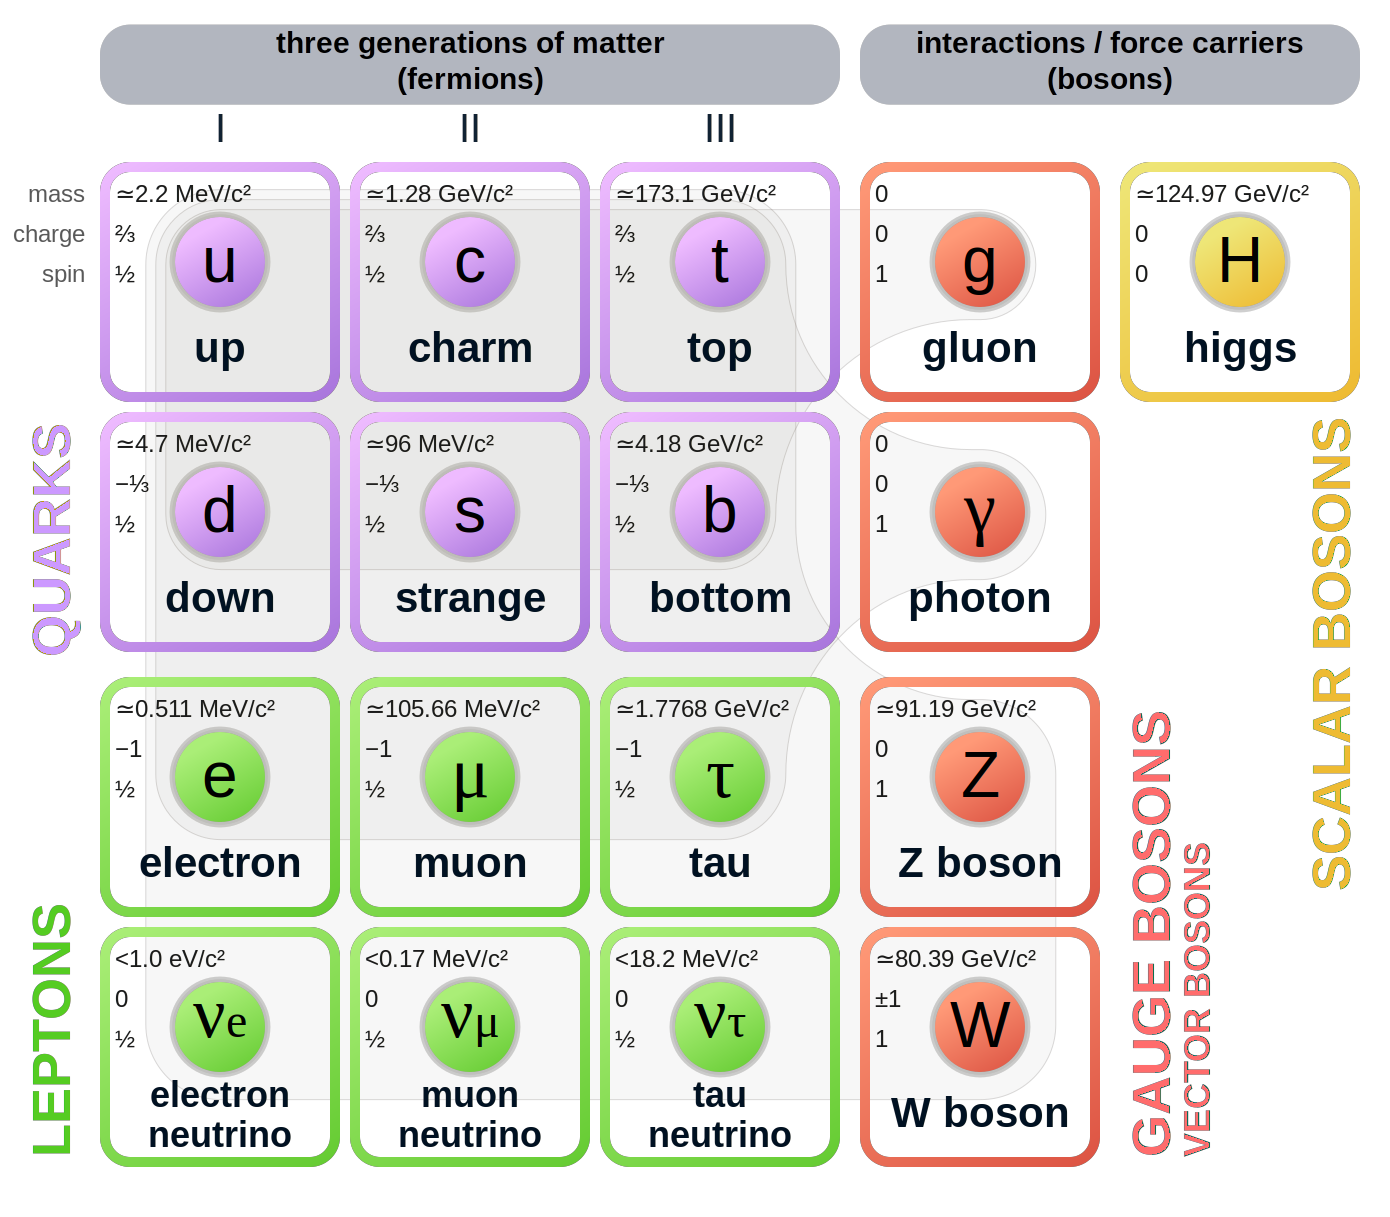
\includegraphics[width=0.6\textwidth]{figures/theoryFigs/SM_particles.png}
\centering
\caption{A summary of the elementary particles described by the SM~\cite{SM-picture} is shown. Fermions are shown on the left, with quarks shown in purple and leptons shown in green. Bosons are shown on the right, with gauge bosons shown in red and the Higgs boson shown in yellow. The mass, electric charge and spin of each particle is shown on the top left of each particle's block.}
\label{fig:SM-particles}
\end{figure}
\noindent
Particles in the SM are uniquely described by their quantum numbers: electric charge and spin. The SM particles are split into main two classes, based off their spin quantum numbers. Particles which have half-integer spin are called fermions, and those which have integer spin are called bosons. Fermions are further divided into three generations, each comprising of two quarks, one charged lepton and one neutrino. In a generation, the more massive quark has an electric charge of $+2/3$ (up-type) and the less massive quark has an electric charge of $-1/3$ (down-type). All charged leptons have an electric charge of $-1$ and all neutrinos are electrically neutral. The masses of the particles in a generation increase with increasing generation number, with generation 1 particles being the least massive and generation 3 particles being the most massive. Quarks carry electric and colour charge, and can therefore interact via the electromagnetic, weak and strong forces. Colour charge can take on three values: red, green and blue. It is important to note that colour charge is completely unrelated to the everyday meaning of colour, and it just represents the quantum state of the particle. Due to colour confinement~\cite{quark-confinement}, quarks cannot be isolated from one another. They exist in colourless bound states, called hadrons, consisting of two or more quarks. Hadrons consisting of an even number of quarks are known as mesons and those consisting of an odd number of quarks are known as baryons. On the other hand, charged leptons (electron ($e$), muon ($\mu$) and tau ($\tau$)) only carry electric charge and can therefore interact electromagnetically and weakly, but not through the strong interaction. The electric and colour neutral fermions, neutrinos, can only interact via the weak force.\\

\noindent
Particles are able to interact with one-another via the exchange of a gauge boson (boson with spin-1). Photons are massless, spin-1 gauge bosons which mediate electromagnetic interactions between particles which carry electric charge, such as quarks and charged leptons ($e$, $\mu$ and $\tau$). The weak interaction is mediated by three massive gauge bosons, the electrically charged $W^{+}$ and $W^{-}$ bosons and the electrically neutral $Z$ boson. Gluons are massless, spin-1 gauge bosons which mediate strong interactions between particles which carry colour charge, such as quarks. Since gluons carry colour charge, they interact with themselves. The massive, spin-0, electrically neutral Higgs boson mediates the Higgs field which gives mass to the $W^{\pm}$ and $Z$ bosons via the so-called Brout-Englert-Higgs mechanism~\cite{PhysRevLett.13.321, Higgs:1966ev, Higgs:1964pj}. The Brout-Englert-Higgs mechanism induces spontaneous electroweak symmetry breaking to provide mass terms for the $W^{\pm}$ and $Z$ bosons in the electroweak Lagrangian of the SM. All particles described in the SM have their own antiparticle, with the same mass, but opposite charges. Some particles, such as the photon, are their own antiparticle.\\

\noindent
Although the SM has shown to be hugely successful, it is incomplete and fails to describe certain observed phenomena. The most notable example being the absence of gravity from the SM. The gravitational force is $\approx 10^{29}$~\cite{thomson2013modern} weaker than the weak force, therefore quantum gravitational effects are expected to only become significant at energies much larger than that currently accessible by the LHC (known as the Planck scale $\approx 10^{9}$ GeV)~\cite{hierarchy-problem-paper}. This large difference in strength between the weak force and gravity is known as the Hierarchy Problem. Cosmological observations infer that around 84$\%$ of the matter in the universe consists of gravitationally interacting matter known as dark matter~\cite{Jarosik_2011}. None of the particles described in the SM are good dark matter candidates, therefore the SM only accounts for a small fraction of the total matter of the universe. The large discrepancy between the observed amount of matter and antimatter in the universe, sometimes referred to as the matter-antimatter asymmetry, is not fully explained by the SM. Neutrinos in the SM are assumed to be massless, however observations of neutrino oscillations (neutrinos undergoing flavour change as they travel through space) imply that neutrinos do have mass~\cite{fantini2020formalism}. Beyond the Standard Model (BSM) theories attempt to explain the phenomena which the SM cannot. For example, a popular extension to the SM, Supersymmetry (SUSY) introduces new particles to the SM which are counterparts to the existing SM particles with the same quantum numbers, except for their spins~\cite{kirsten2010introduction}. SUSY provides elegant explanations to many shortcomings of the SM, however none of the supersymmetric particles described by SUSY have been observed experimentally~\cite{CANEPA2019100033}.

\subsection{The Top Quark}
The top quark is the heaviest particle in the SM, with a mass of 172.76 $\pm$ 0.30 GeV~\cite{pdg}. According to the SM, since the coupling to the Higgs boson is proportional to the the mass of the interacting particle, the top quark is strongly coupled to the Higgs boson. Physics processes involving top quarks is therefore a theoretically well-motivated area to search for new physics, since it is the most likely particle to couple to new physics theories at the TeV scale. Its large mass also makes it highly unstable, with a mean lifetime of $\approx 0.5 \times 10^{-24}$ s~\cite{pdg}. The top quark's lifetime is shorter than that of the hadronisation process, and it therefore decays before hadronising. The top quark can therefore be measured indirectly via its decay products. Top quarks almost always decay to a $W$ boson and a $b$-quark ($\frac{\Gamma(Wb)}{\Gamma( Wq (q=b,s,d))} = 0.957\pm 0.034$~\cite{pdg}). The $b$-quark is the second heaviest quark in the SM, however its lifetime is still longer than the hadronisation time scale~\cite{pdg}. In hadron collider experiments, $b$-quarks travel a short distance in the detector before hadronising to form jets. In Table \ref{tab:top-decay-modes}, the dominant final state branching fractions of the top quark are shown.

\begin{table}[h!]
\def\arraystretch{1.5}%
\begin{tabular}{l|c}
\hline
Decay Mode & Branching Fraction ($\frac{\Gamma_{i}}{\Gamma}$)\\ \hline
$t \rightarrow Wb \rightarrow e\nu_{e} b$           &      $(11.10\pm 0.30)\%$     \\
$t \rightarrow Wb \rightarrow \mu \nu_{\mu} b$             &   $(11.40\pm 0.20)\%$        \\
       $t \rightarrow Wb \rightarrow \tau \nu_{\tau} b$      &  $(10.70\pm 0.50)\%$         \\
  $t \rightarrow Wb\rightarrow q\bar{q} b$           &      $(66.50\pm 1.40)\%$     \\ \hline
\end{tabular}
\centering
\caption{The dominant final state branching fractions of the top quark~\cite{pdg} are shown.}
\label{tab:top-decay-modes}
\end{table}

\noindent
Hadronic final states are more than twice as likely than leptonic final states. Final state decays to different lepton flavours are roughly equally probable.\\

\noindent
Top quark production can be placed into two main categories: pair production ($t\bar{t}$) and single-top production ($t$)~\cite{dasilva2016quark}. In the LHC, top quarks are mainly produced in pairs via strong interactions in gluon-gluon fusion ($gg\rightarrow t\bar{t}$) or quark annihilation ($q\bar{q}\rightarrow t\bar{t}$). Top quark production via gluon-gluon fusion is the dominating process~\cite{Ball_2015}. The production cross section for $t\bar{t}$ (leptonic final state) in $pp$ collisions with $\sqrt{s} = 13$ TeV was measured by ATLAS with a value of $830 \pm 0.4 (\text{stat}) \pm 36 (\text{syst}) \pm 14 (\text{lumi})$ pb~\cite{ATLAS-tt-crossSection-2020}, with good agreement between measurement and theoretical prediction.\\

\noindent
Single top production occurs via the weak interaction. The most abundant production mechanisms leading to single top production are the $s$-, $t$- and $Wt$- channels~\cite{pdg}. In the $s$-channel, an initial quark annihilates with an anti-quark of different flavour, producing a virtual $W$ boson which decays to a top quark and anti-bottom quark. In the $t$-channel, an initial $b$ quark interacts with a different flavour quark via the exchange of a $W$ boson. This interaction produces a top quark and another quark. In the $Wt$-channel, an initial gluon interacts with a $b$ quark to produce a top quark and a $W$ boson, either via the absorption of the gluon by the $b$ quark or via the exchange of a top quark. In Table \ref{tab:single-top-crossSection}, single top production cross sections in $pp$ collisions at $\sqrt{s}=13$ TeV for the $s$-, $t$- and $Wt$-channels, are shown.


\begin{table}[h!]
\def\arraystretch{1.5}%
\begin{tabular}{c|c|c}
\hline
Channel & Process & Total Cross Section [pb] \\ \hline
$s$& $q\bar{q'}\rightarrow   W \rightarrow \bar{b}t$& $10.32^{+0.40}_{-0.36}$  \\
$t$ & $bq'\rightarrow W \rightarrow tq$ &  $216.99^{+9.04}_{-7.71}$\\
$Wt$& $bg \rightarrow  b/t \rightarrow Wt$ &  $71.7\pm 3.85$\\ \hline
\end{tabular}
\centering
\caption{Single top production cross sections in $pp$ collisions at $\sqrt{s}=13$ TeV for the $s$-, $t$- and $Wt$-channels~\cite{summaryPlots} are shown. The prime superscript on $q^{'}$ indicates that the quark has a different flavour to $q$. }
\label{tab:single-top-crossSection}
\end{table}
\noindent
Single top production is suppressed compared to pair produced top production, with $t\bar{t}$ production (leptonic final state) being around three times as likely to occur than single top production across all decay channels.


\subsubsection{Motivation for the search for $tWZ$ production in the tetralepton channel}
The recent lack of signs of new physics from LHC data~\cite{sonneveld2019searches} tells us that new physics is either very heavy, or is very weakly coupled to SM particles. We therefore might only observe signs of new physics in anomalous rates of well-chosen processes. The $tWZ$ process is a prime example of such a process. It has an extremely low production cross section (0.7 fb for $\sqrt{s}= 13$ TeV~\cite{twz-theory-paper}), and has subsequently never been observed by any particle physics experiment. Since $tWZ$ involves a charged $W$ boson and neutral $Z$ boson, its cross section is sensitive to the charged and neutral couplings to the top quark. In turn, the top quark is strongly coupled to the Higgs boson, due to its large mass. Due to the top quark's large coupling to the Higgs boson, corrections to the Higgs boson mass diverge in the SM. The top quark's couplings are modified, in order to remove this divergence, in many scenarios of new physics that aim to resolve the Hierarchy Problem. Since the $Z$ boson may be radiated from the initial-state $b$-quark, the final-state top quark, or the final-state $Z$ boson, the $tWZ$ process embeds the $b-Z$, $t-Z$ and $W-Z$ electroweak couplings which are often modified in BSM physics. Therefore $tWZ$ is an important process in the search for signs of new physics and BSM physics.\\ %\cite{Chaichian_1995}???

\noindent
One such BSM theory which is sensitive to $tWZ$ production~\cite{Maltoni_2019, mimasu2021quark} is the Standard Model Effective Field Theory (SMEFT)~\cite{Brivio_2019}. The SMEFT attempts to describe physics at large energy scales which we have not yet been able to probe experimentally. The SMEFT inherits the same QFT framework as the SM, and adds Lagrangian terms to the SM Lagrangian which describe the interactions of SM particles at higher energy scales. Analogous to the coupling constants found in the SM Lagrangian, which indicate the interaction strengths between different particles, SMEFT contains scalar coefficients which operate in the same way. These scalar coefficients are known as Wilson coefficients. It has been shown that the cross section of $tWZ$ is sensitive to many Wilson coefficients. An experimental constraint on the cross section of $tWZ$ is therefore expected to be impactful on a global fit on all the Wilson coefficients in SMEFT.\\

\noindent
Prior to this analysis, only three experimental studies of $tWZ$ in ATLAS have been performed. The first and third studies utilised the trilepton channel to search for $tWZ$ production, whereas the second study utilised both the tri- and tetralepton channels. The first search utilised 36 fb$^{-1}$ of ATLAS data and an upper limit on the cross section of $tWZ$ was set at a value of $\approx$ 6 times the SM cross section~\cite{twz_3_lep}. The second study investigated the feasibility of a cross section measurement of $tWZ$ production with CMS Run 3 data (300 fb$^{-1}$)~\cite{Tschida:2020ftz}. The study showed that it is possible to exclude $\mu (tWZ)$ at the $7\sigma$ significance level using 300 fb$^{-1}$ of data. This study needs to be further investigated, since its findings seem improbable given the results obtained in this thesis. The third search utilised 139 $^{-1}$ of ATLAS data and an expected upper limit on the cross section of $tWZ$ was set at a value of $\approx$ 2.6 times the SM cross section~\cite{ben-thesis}. In Section \ref{sec:combined-results}, the latter analysis will be used in combination with this analysis, in order to further increase the sensitivity of the cross section of $tWZ$.



%\section{Effective Field Theory (EFT)}
%Brief overview of EFT. What is EFT? Why important to pp as a whole? Why important in twz (high sensitivity to wilson coefficients, expected to have a large impact on global fit)? Similar to what james says in INT note.
%\section{Machine Learning in the Context of Particle Physics Analyses}
%Brief overview of ML as a whole; History; increase in popularity in recent years (why increased in popularity $\rightarrow$ novel techniques developed, increase in computing power for your buck). Where does it fit into pp (event selection, object reconstruction and ID (jet reco, b-tagging)). Explain concepts (vocabulary), overtraining, training, testing, classifier, classification. Why use x train/test ratio in pp (use some for analysis/use some for training)? Popular tools which are used today (scikit learn, TMVA, xgboost what is theano, what is keras).\\
%Maybe a subsection on bdt (if end up using it) on the specific algorithm, and minimizing cost function (general). Explanation on ROC curve and why we can use it as a proxy to determine how well our bdt/nn is doing (and where it fails/can fail $\rightarrow$ things to be aware of cautious of when straight up using ROC integral (e.g. overtraining )).
%\section{Statistical Techniques}
%Brief overview: frequentist and bayes approach in general in pp, why we use frequentist in this analysis



\section{$tWZ$}
\subsection{Tetralepton Channel}
In Figure \ref{fig:twzfourlep_FeymanDiagram}, the Leading Order (LO) Feynman diagram for \tWZ in the tetralepton channel, is shown.

\begin{figure}[h!]
	
\centering
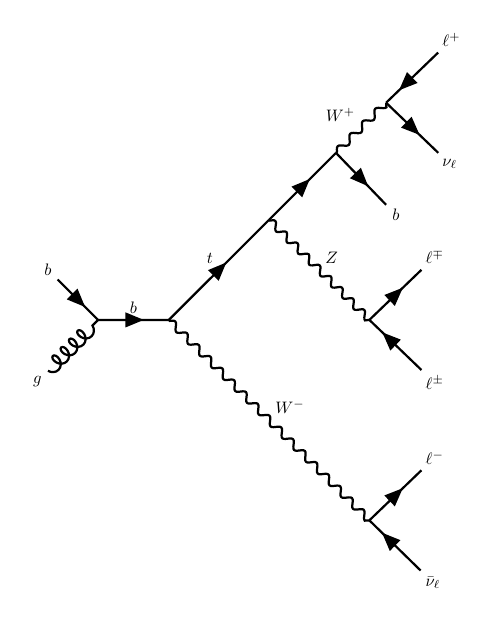
\begin{tikzpicture}[thick,scale=0.6, every node/.style={transform shape}]

\begin{feynman}
\vertex (a) {$b$};
\vertex [below right=of a] (c);
\vertex [below left=of c] (b) {$g$};

\vertex [right=of c] (d);  %d: tW vertex

\vertex [above right=3cm of d] (e);  %e: top vertex

\vertex [below right=3cm of e] (i);  %i: Z -> ll vertex
\vertex [above right=of i] (f1) {$\ell^{\mp}$}; 
\vertex [below right=of i] (f2) {$\ell^{\pm}$}; 


\vertex [above right=2cm of e] (f);  %f: Wb vertex
\vertex [below right=of f] (f7) {$b$};

\vertex [above right=of f] (g);  %g: l \nu vertex
\vertex [below right=of g] (f3) {${\nu}_{\ell}$};
\vertex [above right=of g] (f4) {$\ell^{+}$};


\vertex  [below right=6cm of d] (h); %h: l \nu vertex (bottom)
\vertex [below right=of h] (f5) {$\bar{\nu}_{\ell}$};
\vertex [above right=of h] (f6) {$\ell^{-}$};



\diagram* {
	(a) -- [fermion] (c),
	(b) -- [gluon] (c),
	(c) -- [fermion, edge label=$b$] (d),
	(d) -- [fermion, edge label=$t$] (e),
	
	(e) -- [boson, edge label=$Z$] (i),
	(i) -- [fermion] (f1),
	(i) -- [anti fermion] (f2),
	
	(f) -- [boson, edge label=$W^{+}$] (g),
	(e) -- [fermion] (f),
	(f) -- [fermion] (f7),
	(g) -- [fermion] (f3),
	(g) -- [anti fermion] (f4),
	

	
	(d) -- [boson, edge label=$W^{-}$] (h),
 	(h) -- [anti fermion] (f5),
	(h) -- [fermion] (f6),
	
	
};
\end{feynman}

\end{tikzpicture}
\caption{The LO Feynman diagram of \tWZ production in the tetralepton channel is shown.}
\label{fig:twzfourlep_FeymanDiagram}
\end{figure}



\subsubsection{Backgrounds}
The main backgrounds for \tWZ (tetralepton channel) are the production of a two tops, both in the $\ell \nu b$~\footnote{In this thesis, $\ell$ refers to an electron or muon, $\nu$ refers to a neutrino or anti-neutrino and $b$ refers to a bottom quark or anti-bottom quark} final state channel, together with a $Z$ boson (\ttZ) and diboson production with fully leptonic final states (\ZZ). In Figure \ref{fig:ttz_and_zz_feynman}, LO Feynman diagrams for \ttZ and \ZZ in the tetralepton channel, are shown.

\begin{minipage}{.5\textwidth}
	\centering
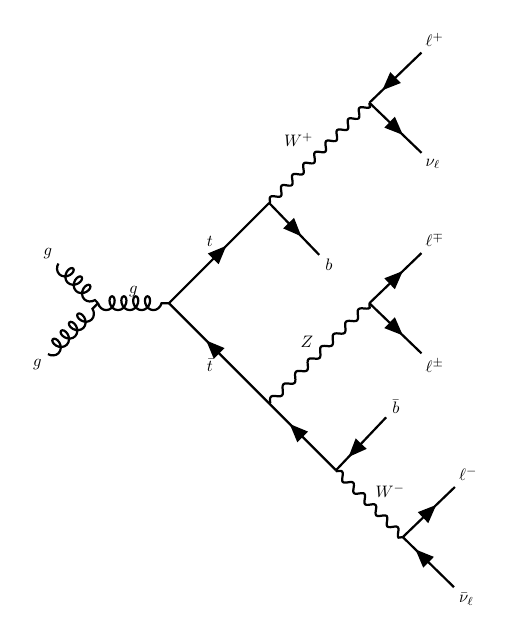
\begin{tikzpicture}[thick,scale=0.6, every node/.style={transform shape}]


\begin{feynman}

\vertex (a) {$g$};
\vertex [below right=of a] (c);
\vertex [below left=of c] (b) {$g$};

\vertex [right=of c] (d);   %g -> ttbar vertex

\vertex [above right=3cm of d] (e);   %d: t-> Wb vertex
\vertex [below right=3cm of d] (f);   %e: t bar-> Z tbar vertex

%t-> Wb vertex
\vertex [above right=3cm of e] (g);  %(g): W-> l\nu (top)
\vertex [above right=of g] (f1)  {$\ell^{+}$};  
\vertex [below right=of g] (f2)  {$\nu_{\ell}$}; 
\vertex [below right=of e] (f3)  {$b$};   

\vertex [above right=3cm of f] (h);   %(h): Z-> ll vertex 
\vertex [above right=of h] (f4) {$\ell^{\mp}$}; 
\vertex [below right=of h] (f5)  {$\ell^{\pm}$}; 


\vertex [below right=2cm of f] (i);   %(i): tbar-> bW
\vertex [above right=of i] (f6)  {$\bar{b}$};  
\vertex [below right=2cm of i] (j);   %W-> l\nu vertex (tbar)
\vertex [above right=of j] (f7)  {$\ell^{-}$};  
\vertex [below right=of j] (f8)  {$\bar{\nu}_{\ell}$}; 





\diagram* {
	
	(a) -- [gluon] (c),
	(b) -- [gluon] (c),
	
	(c) -- [gluon, edge label=$g$] (d),
	
	(d) -- [fermion, edge label =$t$](e),
	(d) -- [anti fermion, edge label'=$\bar{t}$](f),
	
	(e) -- [boson, edge label=$W^{+}$] (g),
	(e) -- [fermion] (f3),
	(g) -- [anti fermion] (f1),
	(g) -- [fermion] (f2),
	
	(f) -- [boson, edge label=$Z$] (h),
	(h) -- [fermion] (f4),
	(h) -- [fermion] (f5),
	
	(f) -- [anti fermion] (i),
	(i) -- [anti fermion] (f6),
	(i) -- [boson, edge label=$W^{-}$] (j),
	(j) -- [fermion] (f7),
	(j) -- [anti fermion] (f8),
	
	
	
	
	
};
\end{feynman}
\end{tikzpicture}
\end{minipage}% This must go next to `\end{minipage}`
\begin{minipage}{.5\textwidth}
	\centering
	\begin{tikzpicture}[thick,scale=0.6, every node/.style={transform shape}]
	\label{fig:zz_FeymanDiagram}
	
	\begin{feynman}
	
	\vertex (a) {$q$};
	\vertex [below right=of a] (c);
	\vertex [below left=of c] (b) {$\bar{q}$};
	
	\vertex [above right=3cm of d] (e); % Z vertex (top)
	\vertex [above right=of e] (f1) {$\ell^{\mp}$}; 
	\vertex [below right=of e] (f2) {$\ell^{\pm}$}; 
	
	
	\vertex [below right=3cm of d] (f); % Z vertex (bottom)
	\vertex [above right=of f] (f3) {$\ell^{\mp}$}; 
	\vertex [below right=of f] (f4) {$\ell^{\pm}$}; 
	
	
	
	
	\diagram* {
		
		(a) -- [fermion] (c),
		(b) -- [anti fermion] (c),
		
		(c) -- [boson, edge label=$Z/ \gamma$] (d),
		
		(d) -- [boson, edge label=$Z$] (e),
		(d) -- [boson, edge label=$Z$] (f),
		
		(e) -- [fermion] (f1),
		(e) -- [anti fermion] (f2),
		
		(f) -- [fermion] (f3),
		(f) -- [anti fermion] (f4)
		
			
	};
	\end{feynman}
	\end{tikzpicture}

\end{minipage}
\label{fig:ttz_and_zz_feynman}
\captionof{figure}{LO Feynman diagrams for \ttZ (left) and \ZZ (right) in the tetralepton channel are shown.}
\vspace{1cm}
The $t\bar{t}Z$ process contains fours leptons and two $b$-quarks in its final state (inclusive $\sigma(t\bar{t}Z)= 0.95 \pm 0.08_{\text{stat}} \pm 0.10_{syst}$ pb at $\sqrt{s}=13$ TeV~\cite{ttz-xsec-paper}) and can easily mimic the \tWZ signal process, for instance, by one of its $b$-jets getting missed during detection. The \ZZ process contains four leptons and zero $b$-quarks in its final state (inclusive $\sigma(ZZ)= 14.6^{+1.9}_{-1.8}(\text{stat})^{+0.5}_{-0.3}(\text{syst})\pm 0.2 (\text{theo})\pm 0.4 (\text{lumi})$ pb at $\sqrt{s}=13$ TeV~\cite{zz-xsec-paper}). One way in which \ZZ can mimic the \tWZ signal process is by reconstruction of a non-prompt $b$-jet. 



\subsection{Comparison to Trilepton Channel}

%Less backgrounds to deal with (in tetralepton). However lower stats (in tetra). Give cross sections (and feynman diagram). Maybe talk a bit about analysis related challenges (trilepton has a hadronically decaying W, does this make the analysis easier or more difficult?).


\begin{figure}[h!]
	
	\centering
	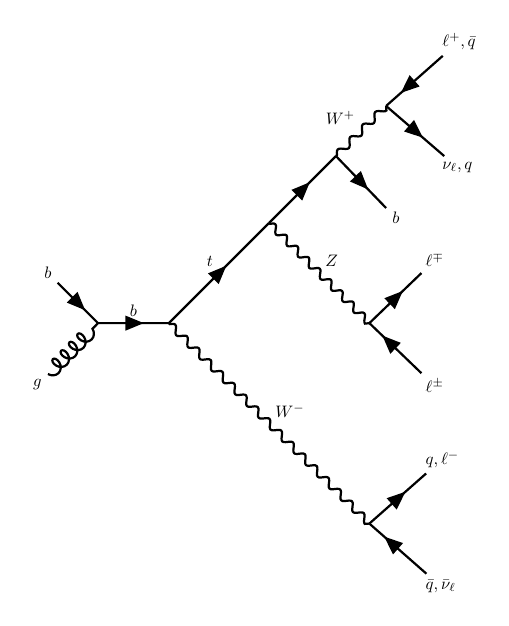
\begin{tikzpicture}[thick,scale=0.6, every node/.style={transform shape}]
	\label{fig:twz3lep_FeymanDiagram}
	\begin{feynman}
	\vertex (a) {$b$};
	\vertex [below right=of a] (c);
	\vertex [below left=of c] (b) {$g$};
	
	\vertex [right=of c] (d);  %d: tW vertex
	
	\vertex [above right=3cm of d] (e);  %e: top vertex
	
	\vertex [below right=3cm of e] (i);  %i: Z -> ll vertex
	\vertex [above right=of i] (f1) {$\ell^{\mp}$}; 
	\vertex [below right=of i] (f2) {$\ell^{\pm}$}; 
	
	
	\vertex [above right=2cm of e] (f);  %f: Wb vertex
	\vertex [below right=of f] (f7) {$b$};
	
	\vertex [above right=of f] (g);  %g: l \nu vertex
	\vertex [below right=of g] (f3) {${\nu}_{\ell}, q$};
	\vertex [above right=of g] (f4) {$\ell^{+}, \bar{q}$};
	
	
	\vertex  [below right=6cm of d] (h); %h: l \nu vertex (bottom)
	\vertex [below right=of h] (f5) {$\bar{q}, \bar{\nu}_{\ell}$};
	\vertex [above right=of h] (f6) {$q, \ell^{-}$};
	
	
	
	\diagram* {
		(a) -- [fermion] (c),
		(b) -- [gluon] (c),
		(c) -- [fermion, edge label=$b$] (d),
		(d) -- [fermion, edge label=$t$] (e),
		
		(e) -- [boson, edge label=$Z$] (i),
		(i) -- [fermion] (f1),
		(i) -- [anti fermion] (f2),
		
		(f) -- [boson, edge label=$W^{+}$] (g),
		(e) -- [fermion] (f),
		(f) -- [fermion] (f7),
		(g) -- [fermion] (f3),
		(g) -- [anti fermion] (f4),
		
		
		
		(d) -- [boson, edge label=$W^{-}$] (h),
		(h) -- [anti fermion] (f5),
		(h) -- [fermion] (f6),
		
		
		
		
	};
	\end{feynman}
	
	\end{tikzpicture}
	\caption{Example Feynman diagram of \tWZ production in the tri-lepton channel.}
\end{figure}

The most apparent difference between the tri and tetralepton channels is the number of events present, with the tetralepton channel having far less events in its phase space than that of the tri-lepton channel. The lack of statistics in the tetralepton channel can be attributed to its low production cross section, $\sigma^{\text{NLO}}_{(tW^{\pm}Z).Br(4\ell)} = \SI{0.7}{fb}$~\cite{twz-theory-paper}. The tri-lepton channel has a production cross section ($\sigma^{\text{NLO}}_{(tW^{\pm}Z).Br(3\ell)} = \SI{3.9}{fb}$~\cite{twz-theory-paper}) around a factor of 4 larger than that of the tetralepton channel. This difference between the production cross section of the two decay channels can be largely attributed to the difference in branching ratios ($\frac{\Gamma_i}{\Gamma}$) between a hadronically decaying $W$ boson, $\frac{\Gamma_{W \rightarrow had}}{\Gamma_W} = (67.41 \pm 0.27) \%$~\cite{pdg}, present in the tri-lepton channel and a leptonically decaying $W$ boson, $\frac{\Gamma_{W \rightarrow \ell^{\+} \nu}}{\Gamma_W}  = (10.86 \pm 0.09) \%$~\cite{pdg}, present in the tetralepton channel.\\

Despite the tetralepton channel's low statistics, it is not subject to the large $WZ$ background present in the trilepton channel~\cite{ben-thesis}. The tetralepton channel has a substantial amount of $ZZ$ background (not present in the trilepton channel), fortunately this can be easily suppressed due to the full reconstructability of the two leptonically decaying $Z$-bosons.











\chapter{The ATLAS Experiment and Detector}
\section{The ATLAS Experiment}
ATLAS (A Toroidal LHC ApparatuS) is one of two general purpose detectors at CERN (the European Organization for Nuclear Research) near Geneva in Switzerland. These detectors collect data from the collisions provided by the worlds highest energy particle accelerator~\cite{lhc-design-report}, the Large Hadron Collider (LHC) situated at CERN. \\

In this section, information about the LHC and the ATLAS detector are given. This includes technical aspects of the ATLAS detector and the processing of data into meaningful physics objects to be used in analyses.

\subsection{Large Hadron Collider (LHC)}
The LHC is a circular 27km particle accelerator located in an underground tunnel on the border between France and Switzerland. The accelerator consists of supercooled, superconducting magnets which accelerate and collide beams of protons at centre-of-mass energies up to $\sqrt{s} = 13$TeV at instantaneous luminosities of $\mathcal{L} \sim 10^{34}$cm$^{-2}$s$^{-1}$. The LHC mainly produces these $pp$ collisions, however heavy-ion collisions can be produced (typically lasting a month, annually) which reach centre-of-mass energies of $\sqrt{s} = 5.02$TeV$/$nucleon at instantaneous luminosities of $\mathcal{L} \sim 10^{27}$cm$^{-2}$s$^{-1}$. $pp$ beams consist of bunches of protons which collide every 25ns, corresponding to a frequency of 40MHz. \\ 

Several accelerator systems are used to accelerate protons and heavy ions to such high energies. Protons are extracted from a tank of ionised hydrogen gas and are injected into the Linear Accelerator 2 (LINAC), where they are linearly accelerated to momenta of 50MeV. The proton bunches are then sequentially accelerated by a chain of circular accelerators. The chain starts with the Booster which accelerates the protons to momenta of up to 1.4GeV. The proton bunches are then fed through to the Proton Synchrotron (PS) and the Super Proton Synchrotron (SPS) which accelerate the protons to momenta of up to 25GeV and 450GeV respectively. The protons are then transferred to two beam pipes of the LHC where they travel in opposite directions. Both proton beams are accelerated to their final momenta of 6.5TeV, resulting in a centre-of-mass energy of 13TeV. These proton beams then collide at one of the four main interaction points situated along the LHC. \\

The four main experiments located at the interaction points are ATLAS, the Compact Muon Solenoid (CMS), Large Hadron Collider Beauty (LHCb) Experiment and A Large Ion Collider Experiment (ALICE). ATLAS and CMS are general-purpose detectors which investigate a wide range of physics processes. Since both ATLAS and CMS can measure the same processes, they are able to cross-check and validate measurements taken by one another. LHCb is specifically designed to study decays of particles containing $b$-quarks. ALICE is designed to study the strongly interacting quark-gluon plasma which is formed at extremely high energy densities.\\

At the interaction points, the two proton beams which consist of protons in closely packed bunches, travel in opposite directions to one another and collide. We are only able to study one $pp$ collision (event) at a time, however many hard $pp$ collisions can occur per bunch crossing. These additional collisions are referred to as \textit{pile-up}. Pileup complicates the reconstruction of the particles originating from the hard collision of interest. 



\section{The ATLAS Detector}
The ATLAS detector is a general purpose particle detector, located at one of the four interaction points along the LHC beam pipe (100 m below ground). In Figure~\ref{fig:atlas-detector}, the schematic of the ATLAS detector, is shown.


\begin{figure}[h!]
 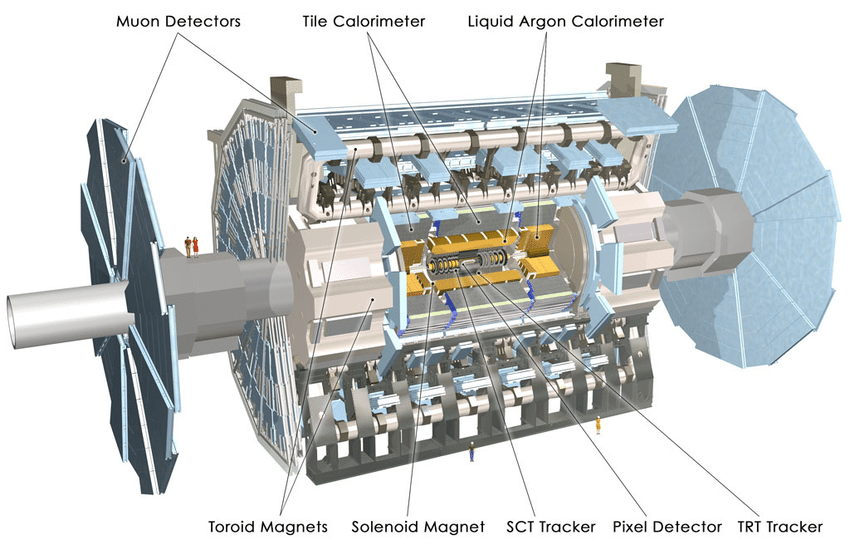
\includegraphics[width=0.5\textwidth]{figures/theoryFigs/atlasDetector.png}
 \centering
\caption{Schematic of the ATLAS detector~\cite{Collaboration_2008}}
\label{fig:atlas-detector}
\end{figure}


The detector is cylindrically shaped which covers close to 4$\pi$ in solid angle. It has a length of 44 m, a diameter of 25 m and a mass of 7000 tons. ATLAS consists of four main sub-detectors arranged in concentric cylindrical layers around the beam pipe. These include the inner detector, the electromagnetic calorimeter, the hadronic calorimeters and the muon spectrometer. The sub-detectors record the momenta, energies and trajectories of different particles produced in the collider, allowing for the reconstruction and identification of these particles to be used in physics analyses.

\subsection{Coordinate System and Kinematics}

The ATLAS detector adopts a right-handed coordinate system. The origin is at the nominal interaction point with the beam direction defining the $z-$axis. The $x-y$ plane (or transverse plane) is perpendicular to the beam line, with the $x-$axis pointing towards the centre of the LHC ring and the $y$-axis pointing upwards towards the Earth's surface. The azimuthal angle, $\phi \in [-\pi, \pi]$, is measured in the transverse plane with respect to the positive $x-$axis. The polar angle, $\theta \in [0,\pi]$, is measured in the $z-y$ plane with respect to the positive $y-$axis. A quantity called the pseudorapidity, $\eta \in [0,\infty]$ is defined as,

\begin{equation}
\eta = -\ln{\tan{\left(\frac{\theta}{2}\right)}}
\end{equation}
$\eta$ is often used as a measure of the polar angle, instead of $\theta$, since the difference in $\eta$ between two particles, $\Delta \eta$, is invariant under a Lorentz boost in the $z-$direction. The angular distance between two physics objects, $\Delta R$, can be written as,

\begin{equation}
\Delta R = \sqrt{(\Delta\phi)^{2} + (\Delta\eta)^{2}}
\end{equation}
where $\Delta\phi$ is the difference in $\phi$ between the two physics objects of interest. Quantities defined in the transverse plane are often used to describe the kinematics of physics objects in hadron collider experiments. The transverse momentum, $p_{T}$, is defined as,
\begin{equation}
p_{T}= \sqrt{(p_{x})^{2} + (p_{y})^{2}}
\end{equation}
where $p_{x}$ and $p_{y}$ are the $x$ and $y$ components of the physics object's momenta, respectively. The transverse energy, $E_{T}$, is defined as,
\begin{equation}
E_{T} = \sqrt{m^{2} + p_{T}^{2}}
\end{equation}
where $m$ is the invariant mass of the physics object. 

%The energy and momentum in particle collisions are conserved, however the absence of detector elements along the beam line, neutrinos escaping from the detector and unknown initial parton momenta restricts us from fully reconstructing the initial and final state particles. We can however, quantify the amount of transverse momenta which is - possibly go in particle ID section


\subsection{Inner Detector}
The inner detector is the first layer of concentric cylindrical sub-detector layers in the ATLAS detector. It is used to identify charged particles and reconstruct the trajectories of charged particles produced in the collisions via energy deposition in semiconductor material (hits) and the ionisation of gas. It consists of three complementary sub-detectors (in order from nearest to farthest from the beam pipe): the Pixel Detector, the Semiconductor Tracker (SCT) and the Transition Radiation Detector (TRT). The Pixel Detector and SCT are based on semiconductor technology and have the highest granularity of any sub-detector in ATLAS, in order to cope with the high frequency of collisions near the interaction point. The TRT consists of drift tubes (straws) containing a mixture of gas ($70\%$ Xe, $27\%$ CO$_{2}$ and $3\%$O$_{2}$), which allows measurement of the energy deposited by charged particles through the ionisation of the gas. Solenoid magnets surround the inner detector and bend the trajectories of charged particles. The charges and momenta of particles can be inferred from their bent trajectories, which are reconstructed by the hits produced via energy deposition in the Inner Detector.

\subsection{Electromagnetic and Hadronic Calorimeters}
The Electromagnetic Calorimeter (ECAL) and Hadronic Calorimeter (HCAL) surround the Inner Detector, with the ECAL nearer to the beam line. The ECAL and HCAL provide accurate measurements of the energy of particles which interact electromagnetically (e.g. photons and electrons) and hadronically (e.g. jets), respectively. Particles entering the calorimeters interact with the detector material and create either a electromagnetic shower (in the ECAL) or a hadronic shower (in the HCAL), depositing all their energy in the calorimeter cells. The calorimeters consist of an active material and a passive absorber material. Active materials are used to measure the energy deposited by the particles and passive absorber materials induce the electromagnetic and hadronic showers. The ECAL uses liquid argon (LAr) as its active material and lead as its absorber material. The HCAL uses alternating steel absorber layers and plastic scintillating tile layers as its active material. The primary mechanism of energy deposition in the ECAL is through bremsstrahlung (for electrons) and pair production (photons). Hadrons usually deposit a small amount of their energy in the ECAL, and interact via inelastic scattering with the nuclei of the detector material. The hadronic showers (jets) produced in these nuclear interactions travel much further than an electromagnetic shower, and for that reason, the volume of the is designed HCAL occupies a much larger space than that of the ECAL.

\subsection{Muon Spectrometer}
The Muon Spectrometer (MS) is the outermost sub-detector of ATLAS and surrounds the HCAL. Muons traverse through the inner detector and calorimeters, with minimal energy loss, before reaching the MS. The MS consists of trigger and high-precision tracking systems. Large superconducting toroid shaped magnets deflect the incoming muons to measure their trajectories and subsequently their momenta via the curvature of the trajectories. The MS measures muon trajectories as they ionize gas (filled with Ar and CO$_{2}$ gas) in the MS drift chambers.

\subsection{Trigger and Data Acquisition System}
The Trigger and Data Acquisition System (TDAQ) manages and handles the large amount of data produced within the ATLAS detector. In Run 2, $pp$ bunch crossings occur every 25 ns, corresponding to an event rate of 40 MHz~\cite{Collaboration_2008}. The TDAQ system performs a fast preliminary reconstruction to select events with signatures which are interesting for physics analyses. The information collected from these events are permanently stored for offline reconstructon and analysis, and the rest (the vast majority of events) are discarded. The trigger system reduces the 40 MHz data rate to around 1 kHz~\cite{Collaboration_2008}.


\subsection{Particle Identification and Object Reconstruction}

%Particles originating from the hard scatter or from their subsequent decays interact with the various detector materials in each sub-detector. Different particles produce characteristic signatures (detector response) inside these sub-detectors.  Include??

Particles originating from $pp$ collisions, or from their subsequent decays, traverse through the ATLAS detector and interact with its different sub-detectors, producing characteristic electronic signals. These signals are then processed by various algorithms to reconstruct and identify the physics objects (e.g. electrons, muons, jets) in the event. This section outlines the procedures used to define these physics objects.

\subsubsection{Tracks and primary vertices}

The trajectories of charged particles, or tracks, are reconstructed in the ID. First, energy is deposited by charged particles (hits) in pixels or strips, in the Pixel and SCT detectors respectively. Adjacent pixels or strips are grouped together in \textit{energy clusters}. A \textit{space-point} is defined in the 


\chapter{Analysis Setup and Strategy}


In this chapter, the full analysis procedure is presented for $tWZ$ production in the tetralepton channel based on an integrated luminosity of 139 fb$^{-1}$ of data recorded by ATLAS. This includes a description of the data and simulation, definitions of physics objects, event selection and the subsequent definition of signal and control regions used in this analysis. Furthermore, estimation of the fake lepton component using the MC template method is described. A kinematic reconstruction algorithm and various Machine Learning techniques, used to discriminate between signal and background events, are described. An outline of the systematic uncertainties affecting the measurement are presented. Finally, the results of the analysis and a study of the analysis projected to higher luminosities is presented. 


\section{Data and Monte Carlo Simulation}
\subsection{Data Samples}
The $pp$ collision data used in this analysis was collected with the ATLAS detector at the LHC from 2015 to 2018. This data period of data taking is referred to as Run 2. During this period, $pp$ collisions at $\sqrt{s}=13$ TeV, corresponding to an integrated luminosity of 156 fb$^{-1}$, were delivered by the LHC. The ATLAS detector recorded 147 fb$^{-1}$ of this total delivered data. 139 fb$^{-1}$ of the data recorded by ATLAS is considered to be good enough for physics analyses (the data passes certain quality control criteria) and placed into the \textit{Good Runs List}~\cite{goodrunslist}. Specific time-intervals where the luminosity is assumed to be constant are known as \textit{lumi-blocks}. Only events from lumi-blocks in which LHC beams were stable and all ATLAS detectors were operational are selected. The list of suitable run and lumi-blocks is summarised in the official Good Runs Lists for 2015-2018 data, as specified in Ref.~\cite{goodrunslist}. The integrated luminosities corresponding to the individual datasets for years 2015, 2016, 2017 and 2018 are 3.2 fb$^{-1}$, 33.0 fb$^{-1}$, 44.3 fb$^{-1}$ and 58.5 fb$^{-1}$ respectively.


\subsection{Monte Carlo Samples}
\label{sec:mcsamples}
%Signal and Background samples. Choice of cuts at ntuple level. Specifically why each background is chosen (and why others excluded) $\rightarrow$ e.g. talk about branching fractions, cross sections, topology. How are these backgrounds passing our event selection (e.g. ttz $\rightarrow$ b can be lost/untagged/mis-id'ed) $\rightarrow$ provide an explanation for each background. Details of each sample (event generator, parton shower).\\

Simulated Monte Carlo (MC) samples were generated and used to model the SM \tWZ signal and its backgrounds. The following background processes are considered:
\begin{itemize}
	\item $\mathbf{t \bar{t} Z}$: $t \bar{t} $  with an associated $Z$-boson, in the tetralepton final state. Therefore, both top quarks decay leptonically (e.g. $t \rightarrow W^+ b \rightarrow \ell^+ \nu b$) and of these top quarks emits a $Z$-boson which decays leptonically ($Z \rightarrow \ell^\pm \ell^\mp$ (OSSF lepton pair) ). This results in a final state with 4 leptons and 2 b-quarks.
	\item $\mathbf{ZZ}$: Diboson production with a tetralepton final state, therefore both $Z$-bosons decay leptonically ($Z \rightarrow \ell^\pm \ell^\mp$ (OSSF lepton pair) ).
	\item \textbf{other}: Processes with a relatively minimal, but non-negligible background contribution
	\begin{itemize}
	\item [-] $VVV (V=W/Z)$
	\item [-] $t\bar{t}$
	\item [-] $t\bar{t}W$
	\item [-] $t\bar{t}WW$
	\item [-] $t\bar{t}H$
	\item [-] $WZ$
	\item [-] $t\bar{t}t$
	\item [-] $t\bar{t}t\bar{t}$
	\item [-] $tZq$
	\end{itemize}
\end{itemize}The MC simulations are achieved via the use of event generators and parton shower generators. The parton shower generators simulate any incoming or outgoing particles from the hard process, which carry QCD color charge and can therefore lead to parton showers. The production of \tWZ events is simulated with the \texttt{MADGRAPH5$\_$AMC@NLO 2.3.3}~\cite{Alwall:2014hca} generator providing matrix element (ME) calculations at NLO (next-to-leading order) in QCD. The events are interfaced with \texttt{PYTHIA 8.235} for the parton shower. The production of $t\bar{t}Z$ and $t\bar{t}W$ events are simulated with the \texttt{MADGRAPH5$\_$AMC@NLO 2.3.3} generator providing ME calculations at NLO in QCD. The events are interfaced with \texttt{PYTHIA 8.210}~\cite{Sjostrand:2014zea} for the parton shower. Event generation of $tWZ$ and $t\bar{t}Z$ results in diagrams which overlap with one another, that is, these diagrams contain the same initial and final state particles. Several methods exist in order to separate between the two processes, by removing the overlap, therefore avoiding double counting. There are two different diagram removal procedures, diagram removal procedure 1 (DR1)~\cite{Demartin:2016axk} and diagram removal procedure 2 (DR2). The DR1 scheme is used to remove the overlap between $tWZ$ and $t\bar{t}Z$. A comparison to the DR2 scheme is used to estimate part of the theoretical systematic on the modelling of the $tWZ$ signal (See Section \ref{subsec:syst_theory}). Diboson processes which feature the three charged leptons and one neutrino or four charged lepton in their final states, such as $WZ$ and $ZZ$, are simulated using \texttt{SHERPA 2.2.2}~\cite{Bothmann_2019} at NLO in QCD precision. The events are interfaced with \texttt{SHERPA} for the parton shower. Triboson processes such as $WWW$, $WWZ$, $WZZ$, and $ZZZ$ containing up to six leptons in their final states are simulated using \texttt{SHERPA 2.2.2} at NLO in QCD precision. The events are interfaced with \texttt{SHERPA} for the parton shower. The production of $t\bar{t}$ events are simulated with the \texttt{POWHEG}~\cite{Frixione:2007vw} generator providing ME calculations at NLO in QCD. The events are interfaced with \texttt{PYTHIA 8.210} for the parton shower. The production of $t\bar{t}t$, $t\bar{t}t\bar{t}$ and $t\bar{t}WW$ are simulated using the \texttt{MADGRAPH5$\_$AMC@NLO 2.2.2} generator at LO in QCD precision. The events are interfaced with \texttt{PYTHIA 8.186}~\cite{Sjostrand:2007gs} for the parton shower. The production of $t\bar{t}$ with an associated Higgs boson, $t\bar{t}H$, are generated using the \texttt{MADGRAPH5$\_$AMC@NLO 2.6.0} generator at NLO in QCD precision. The events are showered using \texttt{PYTHIA 8.230}~\cite{Sjostrand:2014zea}. The production of $t\bar{t}$ events are simulated with the \texttt{POWHEG} generator providing ME calculations at NLO in QCD. The events are showered using \texttt{PYTHIA 8.230}. The production of a single top quark in association with a $Z$-boson and an extra parton, $tZq$, is simulated using \texttt{MADGRAPH5$\_$AMC@NLO 2.3.3} at NLO in QCD precision. The events are interfaced with \texttt{PYTHIA 8.230} for the parton shower. In Table \ref{tab:evtgen-partshower}, the event generator and parton shower used for each process's sample are shown.

\begin{table}[h!]
\begin{tabular}{cccc}
\hline
Process   & Event Generator & Cross section calculation & Parton Shower \\ \hline
\tWZ &      \texttt{MADGRAPH5$\_$AMC@NLO 2.3.3}      & NLO     &   \texttt{PYTHIA 8.235}  \\
\ttZ &       \texttt{MADGRAPH5$\_$AMC@NLO 2.3.3}   & NLO       &  \texttt{PYTHIA 8.210}   \\
\ZZ, $WZ$  &        \texttt{SHERPA 2.2.2}      &   NLO  &  \texttt{SHERPA}     \\
$VVV (V=W/Z)$ & \texttt{SHERPA 2.2.2} & NLO & \texttt{SHERPA}\\
$t\bar{t}$ & \texttt{POWHEG} & NLO & \texttt{PYTHIA 8.230}\\
$t\bar{t}W$ & \texttt{MADGRAPH5$\_$AMC@NLO 2.3.3} & NLO & \texttt{PYTHIA 8.210}\\
$t\bar{t}WW$ &\texttt{MADGRAPH5$\_$AMC@NLO 2.2.2} & LO& \texttt{PYTHIA 8.186}\\
$t\bar{t}H$ & \texttt{MADGRAPH5$\_$AMC@NLO 2.6.0}& NLO & \texttt{PYTHIA 8.230}\\
$t\bar{t}t$, $t\bar{t}t\bar{t}$ & \texttt{MADGRAPH5$\_$AMC@NLO 2.2.2}  & LO& \texttt{PYTHIA 8.186} \\
$tZq$ & \texttt{MADGRAPH5$\_$AMC@NLO 2.3.3} & NLO & \texttt{PYTHIA 8.230} \\
                  \hline
\end{tabular}
\centering
\caption{The event generator and parton shower used for the signal and background process's MC samples is shown.}
\label{tab:evtgen-partshower}
\end{table}
\subsection{Trigger Strategy}
\label{sec:trigger}

Events in data and simulation are selected via either single lepton or dilepton (electron or muon) triggers. To selected events, a logical \textbf{OR} between the triggers is applied. This means that events have to be selected by at least one of the single or dilepton triggers. Electrons and muons may be surrounded by other particles which could lead to problems in the reconstruction and identification process. They are therefore required to be sufficiently isolated from other particles. This is done by defining an isolation variable which ensures that the summed energies of the particles in a cone defined around the muon, with radius $\Delta R$, are small. The isolation variable for a cone of radius $x$, $I_{\Delta R = x}$, is given by,
\begin{equation}
I_{\Delta R = x} = \frac{\sum_{i} E_{i}}{p^{e/m}_{T}}
\end{equation}
where $E_{i}$ is the energy of the $i^{\text{th}}$ particle within the cone and $p^{e/m}_{T}$ is the $p_{T}$ of the electron or muon. In order to identify an electron or muon, various properties and detector signals related to them are fed into different Machine Learning classifiers to determine the likelihood of the particle being an electron or a muon. Cuts are applied to the output of the classifiers to define working points which correspond to different selection efficiencies. The names commonly given to different working points, in order of decreasing efficiency, are very loose, loose, medium and tight. The single-muon trigger used to select muons in 2015 data and simulation requires a muon with $p_{T} > 20$ GeV, an identification criteria corresponding to a loose working point and $I_{\Delta R = 0.2} < 0.12$. Two single-muon triggers are used to select muons in 2016-2018 data and simulation. The first requires a muon with $p_{T} > 26$ GeV, an identification criteria corresponding to a medium working point and $I_{\Delta R = 0.3} < 0.06$. The second requires a muon with $p_{T} > 50$ GeV. Two single-electron triggers are used to select electrons in 2015 data and simulation. The first requires an electron with $p_{T} > 24$ GeV and an identification criteria corresponding to a medium working point. The second requires an electron with $p_{T} > 120$ GeV and an identification criteria corresponding to a loose working point. Three single leptons triggers are used to select electrons in 2016-2018 data and simulation. The first requires an electron with $p_{T}>26$ GeV, an identification criteria corresponding to a tight working point and $I_{\Delta R = 0.2} < 0.1$. The second requires an electron with $p_{T} > 60$ GeV and an identification criteria corresponding to a medium working point. The third requires an electron with $p_{T} > 140$ GeV and an identification criteria corresponding to a loose working point. The di-muon trigger used to select muons in 2015 data and simulation requires that one muon have $p_{T}> 18$ GeV and another muon to have $p_{T}> 8$ GeV. The di-muon trigger used to select muons in 2016-2018 data and simulation requires that one muon have $p_{T}> 22$ GeV and another muon to have $p_{T}> 8$ GeV. The di-electron trigger used to select electrons in 2015 data and simulation requires two electrons, each with $p_{T} > 12$ GeV, and identification criteria corresponding to loose working points. The di-electron trigger used to select electrons in 2016-2018 data and simulation requires two electrons, each with $p_{T} > 17$ GeV, and identification criteria corresponding to very loose working points. A final electron-muon trigger is used to select electrons and muons in 2016-2018 data and simulation that requires an electron with $p_{T} > 17$ GeV and a muon with $p_{T} > 14$ GeV, and identification criteria corresponding to loose working points. In Table \ref{tab:triggers}, a summary of the triggers used to select muons and electrons in data and simulation are shown.



\begin{table}[!htb]
\footnotesize
\def\arraystretch{1.3}
\begin{center}
\begin{tabular}{ l|l|l }
\hline
\hline
Trigger & Selection [GeV] & Working Point  \\ \hline
Single-muon$*$ & $p_{T} > 20$ & loose\\
Single-muon &  $p_{T} > 26$ & medium \\
Single-muon  &  $p_{T} > 50$ & - \\
Single-electron$*$  & $p_{T} > 24$ & medium \\
Single-electron$*$  & $p_{T} > 120$ & loose \\
Single-electron  & $p_{T} > 26$ & loose \\
Single-electron  & $p_{T} > 60$ & medium \\
Single-electron  & $p_{T} > 140$ & loose \\
Di-muon$*$  & $p_{T} > 18$, $p_{T} > 8$  & - \\
Di-muon  & $p_{T} > 22$, $p_{T} > 8$  & - \\
Di-electron$*$ & $p_{T} > 12$  & loose \\
Di-electron$*$ & $p_{T} > 12$  & loose \\
Di-electron & $p_{T} > 17$  & very loose \\
Electron-Muon & electron $p_{T}> 17$, muon $p_{T} > 14$ & loose\\

\hline
\hline
\end{tabular}
\caption{Single lepton and dilepton (electron and muon) triggers used to select events in data and simulation. Triggers labelled with $*$ are only used for 2015 data and simulation.}
\label{tab:triggers}
\end{center}
\end{table}
\section{Physics objects}
In this section the physics objects (leptons, jets and $b$-tagged jets) used in this analysis are outlined.
\subsection{Leptons}
\label{sec:lepton-object}
In this analysis only $e$ and $\mu$ leptons are considered, since $\tau$ leptons are difficult to detect in the ATLAS detector. They are challenging to detect since they have an extremely short lifetime (290.3 $\pm$ 0.5 fs~\cite{pdg}) which causes them to decay before reaching any detector components and therefore can only be reconstructed via their decay products. In addition to our selection criteria of exactly four leptons, it is required that the Leading (L), Next-to-Leading (NL), Next-to-Next-to-Leading (NNL) and Next-to-Next-to-Next-to-Leading (NNNL) leptons have $p_{T}$ greater than $\SI{28}{}$, $\SI{18}{}$, $\SI{10}{}$ and $\SI{10}{\GeV}$ respectively. Relativity loose object-level cuts are chosen in an attempt to maximize our signal statistics, since the analysis is heavily statistically limited. Reconstructed electrons are required to be within $|\eta| < 2.47$ and excluding the transition region between the barrel and end-cap calorimeters at $1.37 < |\eta| < 1.52$. Reconstructed muons are required to be within $|\eta| < 2.5$. The transverse impact parameter, $d_{0}$, is defined as the minimal spacial distance between the object's (referring to leptons) trajectory and the primary vertex (the vertex associated with the $pp$ hard scatter). The longitudinal impact parameter, $z_{0}$, is defined as the value of $z$ of the point on the object's trajectory which determines $d_{0}$. To ensure consistency between the lepton and the primary vertex, it is required that $|\frac{d_{0}}{\sigma(d_{0})}| < 5$, $|z_{0}\sin{\theta}| < \SI{0.5}{mm}$ for electrons and $|\frac{d_{0}}{\sigma(d_{0})}| < 3$, $|z_{0}\sin{\theta}| < \SI{0.5}{mm}$ for muons, following the current recommendations~\cite{TopRecoObjTwikiModel}. To avoid instances where one detector signal can result in multiple different reconstructed objects, an overlap removal procedure is applied which ignores all but one of these objects (See Section \ref{sec:overlap-removal-procedure}). Electrons are selected using a likelihood based discriminant~\cite{electronRecoAndID:paper} which takes measurements from the tracking system, calorimeter system and quantities derived from both the tracking and calorimeter system as input. Muons are selected using the \texttt{Muon Selection Tool}~\cite{muon-selection-tool}. Loose electrons are defined with the criteria above, using the \texttt{LooseAndBLayerLH} ($\sim$ 91$\%$ selection efficiency for electrons with $E_{T} > \SI{30}{GeV}$~\cite{electronIDefficiency}) identification algorithm (which has a certain cut applied). Similarly, tight electrons are defined with the criteria above, using the \texttt{TightLH} ($\sim$ 80$\%$ selection efficiency for electrons with $E_{T} > \SI{30}{GeV}$~\cite{electronIDefficiency}) algorithm (which has a certain cut applied). Both loose and tight muons use the \texttt{Medium} ($\sim$ 95$\%$ selection efficiency~\cite{muonIDEfficiency}) algorithm (which has a certain cut applied). Tight leptons additionally require that they are sufficiently isolated from other particles produced in the collision. This is done by defining a cone of radius $\Delta R = \sqrt{\Delta \eta^{2} + \Delta \phi^{2}}$ around the particle of interest and summing the $p_{T}$ of all the reconstructed particles surrounding the particle of interest, situated within the cone. A quantity, $I_{rel}$, is then defined as, $I_{rel} = \frac{\Sigma p_{T}(\text{surrounding candidate})  }{p_{T}(\text{candidate})}$, the ratio of this sum to the $p_{T}$ of the lepton candidate. If this value is large, is it likely that the particle of interest originated from a jet (together with many other particles), whereas a prompt decay product resulting from the hard scatter will have little to no energy surrounding it ($I_{rel} \ll 1$). The \texttt{IsolationSelectionTool} with the \texttt{PLVTight} ($\sim$ 70$\%$ efficiency~\cite{elecIsolationEfficiency}) and \texttt{PLVTight} ($\sim$ 70$\%$ efficiency at $p_{T} = \SI{30}{GeV}$~\cite{muonIsolationEfficiency}) algorithm are used for tight electrons and tight muons respectively (following the current recommendations~\cite{recommendedIsolationWPs}). In Table \ref{tab:lepton-selection}, a summary of the selection criteria for leptons is shown.

\begin{table}[htbp]
	\centering
		\resizebox{\textwidth}{!}{%
	\begin{tabular}{c|cc|cc} 
		\toprule
		& \multicolumn{2}{c|}{Electrons }   & \multicolumn{2}{c}{Muons}       \\ \hline
		& Tight    & Loose    & Tight      & Loose        \\ 
		\hline
		$p_{T}$ cuts    & \multicolumn{4}{c}{$p_{T}(\ell_1,\ell_2,\ell_3,\ell_4) > (28,18,10,10)$ $\SI{}{\GeV}$}   \\
		\multicolumn{1}{l|}{Overlap Removal} &\multicolumn{4}{c}{Described in Section \ref{sec:overlap-removal-procedure}}\\  
		$\eta$ cuts       & \multicolumn{2}{c|}{$|\eta(\ell_e)| < \SI{2.47}{}$ excluding $\SI{1.37}{} < |\eta(\ell_e)| < \SI{1.52}{}$} & \multicolumn{2}{c}{$|\eta(\ell_\mu)| < \SI{2.5}{}$~}                                           \\
		\multicolumn{1}{c|}{Impact Parameters} & \multicolumn{2}{c|}{$|\frac{d_{0}}{\sigma(d_{0})}| < 5$,~$|z_{0}\sin{\theta}| < \SI{0.5}{mm}$}             & \multicolumn{2}{c}{$|\frac{d_{0}}{\sigma(d_{0})}| < 3$,~$|z_{0}\sin{\theta}| < \SI{0.5}{mm}$}  \\ 
		Identification WP  & TightLH  & LooseAndBLayerLH      & Medium   & Medium   \\
		Isolation WP & PLVTight & Not Used      & PLVTight  & Not Used  \\
		\bottomrule
	\end{tabular}}
\caption{A summary of the requirements applied for selecting tight and loose leptons ($e,\mu$) is shown.}
\label{tab:lepton-selection}
\end{table}
\subsection{Jets}
Jets are reconstructed using the anti-$k_{t}$ algorithm (See Section \ref{sec:jets-btagging}). The \texttt{AntiKt4EMPFlowjets} ($\sim$ 97$\%$ average efficiency with JVT (outlined in the subsequent paragraph) $>$ 0.2~\cite{TopRecoObjTwikiModel}) algorithm (which has a certain cut applied) is used, following the current recommendations~\cite{TopRecoObjTwikiModel}. The jet-vertex-tagger (JVT) and the forward jet-vertex-tagger (fJVT)~\cite{ATL-PHYS-PUB-2015-034} are likelihood discriminant which aim to suppress pile-up jets. The \texttt{Medium} algorithm (which has a certain cut applied) is used for the JVT and the fJVT (following the current recommendations~\cite{JVTandfJVT-Recommendations}). Additionally, a requirement that jets have a JVT value greater than $\SI{0.5}{}$ is applied. In the same way as with leptons, ambiguities are removed where one detector signal can result in multiple different reconstructed objects, via overlap removal (See Section \ref{sec:overlap-removal-procedure}). Jets are required to be within $p_{T}(\text{jet}) > \SI{20}{\GeV}$. These relatively loose $p_T$ cuts are applied in an attempt to increase our limited signal statistics. A forward jet is a signature of single top quark production, jets are therefore required to have $|\eta| < 4.5$ in order to include these forward jets.

\subsection{$b$-tagging}
The DL1r $b$-tagger~\cite{DL1r-paper} was used to identify jets as $b$-jets (See Section \ref{sec:jets-btagging}). Different DL1r working points are used to identify $b$-jets in our event selection (See Section \ref{sec:regionsAndEventSelection}). The working points are defined as different cuts on the DL1r score corresponding to a $b$-jet tagging efficiency of 60$\%$, 70$\%$, 77$\%$ and 85$\%$. The efficiency of the DL1r $b$-tagger is measured using control samples in data and in simulation. From these measurements, correction factors are derived to correct the tagging rates in the simulation. In the case of $b$-tagged jets, the correction factors and
their uncertainties are estimated from data using dileptonic $t\bar{t}$ events~\cite{PERF-2016-05,FTAG-2018-01}. Sources of uncertainty affecting the $b$-tagging efficiencies are evaluated as a function of jet $p_{T}$, including bin-to-bin correlations. Since this analysis is heavily statistically limited, the amount of statistics in our regions are aimed to be maximized. In an attempt to achieve this goal in the $t\bar{t}Z$ CR, $b$-tagged jets were placed under \textit{tight} and \textit{loose} definitions. A tight $b$-tagged jet is defined as a jet which passes the 77$\%$, 70$\%$, 65$\%$ or 60$\%$ DL1r $b$-tagger working point. A loose $b$-tagged jet is defined as a jet which passes 85$\%$ DL1r $b$-tagger working point, but not the 77$\%$, 70$\%$, 65$\%$ or 60$\%$ DL1r $b$-tagger working points. Different numbers and definitions of tight and loose $b$-tagged jets were tried in each region, with the final selection criteria being chosen which maximised the expected significance of $\sigma(tWZ)$ (See Section \ref{sec:optimization-studies-tetra}).

\subsection{Overlap Removal Procedure}
\label{sec:overlap-removal-procedure}

An overlap removal procedure is performed to avoid instances where one detector signal can result in multiple different reconstructed objects. The overlap removal procedure is used on pre-selected leptons and jets. It is performed sequentially, in the following steps:

\begin{enumerate}
\item If the separation between a pre-selected electron and pre-selected muon is within $\Delta R < 0.01$, or they share a track, the pre-selected electron is discarded.
\item If the separation between a jet and a pre-selected electron is within $\Delta R < 0.2$, the jet is discarded.
\item Any remaining electron or muon closer than $\Delta R = 0.4$ to a jet, is discarded.
\item If the distance between a jet and a pre-selected muon is $\Delta R < 0.4$ and the jet has more than two associated tracks, then the muon is discarded, otherwise the jet is discarded.
\end{enumerate}

\section{Kinematic cuts}
In order to suppress potential fakes and quarkonia (low mass resonances such as $J/\psi$ and upsilon) a requirement that all OSSF lepton pairs have an invariant mass, $m_{\text{OSSF}}$, greater than $\SI{10}{\GeV}$ is applied. The final state lepton charges must sum to zero. Therefore a requirement of $\sum_{i=1}^{4} \text{charge}(\ell_i) = 0$ is applied. The invariant mass of the OSSF lepton pair coming from the $Z$ boson must equal the invariant mass of the $Z$ boson, and noting that $e$,$\mu$ reconstruction and identification in the ATLAS detector has a high efficiency~\cite{Marchese:2688452}, these OSSF leptons are used to reconstruct $Z$ bosons with relatively high confidence. A $Z$ candidate is defined in this analysis as an OSSF lepton pair with an invariant mass, $m_{\text{OSSF}}$, satisfying the condition, $|m_{\text{OSSF}} - m_Z| <  \SI{30}{\GeV}$, where $m(Z)$ is the nominal $Z$ boson mass ($\SI{91.1876}{\GeV}$~\cite{pdg}). This wider mass window is used in order to cover the full range of the $m(Z)$ distribution, in an attempt to increase the number of events which pass our baseline selections. Multiple $Z$ candidates can be present in certain decay channels (e.g. $eeee$, $\mu\mu ee$, $\mu \mu \mu \mu$). In these cases, the $Z$ candidate which has an invariant mass closest to the nominal $Z$ boson mass is chosen. 
\section{Regions and Event Selection}
\label{sec:regionsAndEventSelection}

Two \tWZ SRs are defined in an attempt to suppress and constrain the \ZZ background. Both \tWZ SRs are required to have exactly four tight leptons, exactly one $Z$-boson candidate, exactly one tight $b$-tagged jet (from the decay of the top quark) and greater than or equal to one jet. The two \tWZ SR's differ by the flavours of their leptons which don't originate from the decay of a $Z$-boson (non-$Z$ leptons). The \ZZ background has two $Z$-bosons which decay into a pair of OSSF lepton pairs, in order to mimic the \tWZ signal. This is taken advantage of, to define a \tWZ region enrich in \ZZ background and one with a minimal \ZZ background component. This is done by requiring that one of the \tWZ SRs has its two non-$Z$ leptons to have opposite flavour and the other \tWZ SR is required to have its non-$Z$ leptons to have the same flavour. These two disjoint \tWZ SRs are named \tWZ OF SR and \tWZ SF SR respectively. It is therefore expected that the \tWZ SF SR contains the majority of the \ZZ background events across both \tWZ SRs. In order to check the modelling of the most dominant background components in our signal region, \ttZ and $ZZb$ control regions are defined. The \ttZ control region has the same requirement on the number of reconstructed $Z$ boson candidates in the signal region (due to a commonality on the number of $Z$ bosons present in both processes), however it is required that there are at least two jets and that exactly two of these jets are $b$-tagged (corresponding to the $b$-quark jets originating from the two top quark decays). A $ZZb$ region is defined, as opposed to a \ZZ region, since the \ZZ background present in the $tWZ$ signal region contains exactly one b-tagged jet. Therefore defining a region with \ZZ plus exactly one $b$-jet more closely resembles the $ZZ$ background present in the signal region. In addition to this, mis-modelling of \ZZ has been seen in other analyses~\cite{Aaboud:2019, ppToZZ:CMSpaper}, further motivating the use of a $ZZb$ control region over a \ZZ CR. The $ZZb$ CR requires exactly two $Z$ boson candidates and exactly one b-tagged jet, resulting in an implicit requirement on the number of jets ($N_{jet} \geq 1$).\\

Fake leptons are objects reconstructed as leptons, but do not correspond to the leptons that are of interest in our analysis. Fake leptons can be split up into two main categories, irreducible fakes and reducible fakes. Irreducible fakes are true leptons which do not come from the process of interest. Reducible fakes are objects which are mis-identified or incorrectly reconstructed as leptons. In the ATLAS detector, the probability for a fake to occur is very low. In order to constrain the fake lepton component contained within the \ttZ sample, a $(\tWZ)_{\text{fake}}$ CR is defined which is as similar as possible to the \tWZ SRs but is enhanced in fakes. This is achieved by defining the $(\tWZ)_{\text{fake}}$ CR to inherit the same selection criteria as the \tWZ SRs however, in this case, a requirement of exactly 3 tight leptons and exactly 1 loose (and NOT tight) lepton is applied. Loose leptons are required in this region, since looser leptons are more likely to be fakes compared to tighter leptons. A $(t\bar{t}Z)_{\text{fake}}$ CR, requiring exactly 3 tight leptons and exactly 1 loose (and NOT tight) lepton, was tried as an alternative to the $(\tWZ)_{\text{fake}}$ CR, however a much larger suppression of fakes were observed in this region compared to the $(\tWZ)_{\text{fake}}$ CR. This suppression of fakes can be explained by the extra $b$-tagged jet requirement (exactly two $b$-tagged jets are required in the \ttZ region, compared to exactly one in the \tWZ SRs (See Table \ref{tab:4Lep-cutsummary})) which causes suppression of fakes via the overlap removal procedure (See Section \ref{sec:overlap-removal-procedure}). In Table \ref{tab:4Lep-cutsummary}, a summary of the final selection criteria and region definitions is shown.
\begin{table}[h!]
\centering
\resizebox{\textwidth}{!}{%
\begin{tabular}{ccccc} 
\toprule
\multicolumn{5}{c}{\textbf{Baseline selections}}   \\ 
\midrule
\multicolumn{5}{c}{N$_{\ell} = 4$} \\
\multicolumn{5}{c}{$p_{T}(\ell_1,\ell_2,\ell_3,\ell_4) > (28,10,10,10)$ $\SI{}{\GeV}$} \\
\multicolumn{5}{c}{$p_{T}(\text{jet})> \SI{20}{\GeV}$, $|\eta(\text{jet})| < \SI{4.5}{}$, $\text{jvt} > \SI{0.5}{}$}   \\
\multicolumn{5}{c}{$|\eta(\ell_e)| < \SI{2.47}{}$ excluding $\SI{1.37}{} < |\eta(\ell_e)| < \SI{1.52}{}$}  \\
\multicolumn{5}{c}{$|\eta(\ell_\mu)| < \SI{2.5}{}$}\\
\multicolumn{5}{c}{$\displaystyle\sum_{i=1}^{4} \text{charge}(\ell_i) = 0$}\\
\multicolumn{5}{c}{All OSSF lepton pairs require $m_{\text{OSSF}} > \SI{10}{\GeV}$}\\ 
\midrule
\multicolumn{5}{c}{\textbf{Regions}}   \\ 
\midrule
$tWZ$ OF SR  & $tWZ$ SF SR & $t\bar{t}Z$ CR   & $ZZb$ CR & $(tWZ)_{\text{fake}}$ CR  \\ 
\midrule
\multirow{2}{*}{N$_{\ell}$(tight) $=$ 4} & \multirow{2}{*}{N$_{\ell}$(tight) $=$ 4} & \multirow{2}{*}{N$_{\ell}$(tight) $=$ 4} & \multirow{2}{*}{N$_{\ell}$(tight) $=$ 4} & N$_{\ell}$(tight) $=$ 3   \\
 &   &  &  & N$_{\ell}$(loose and NOT tight) $=$ 1 \\
 &   &  &  &   \\
N$_{\text{Z candidate}} = 1$ & N$_{\text{Z candidate}} = 1$  & N$_{\text{Z candidate}} = 1$ & N$_{\text{Z candidate}} = 2$ & N$_{\text{Z candidate}} = 1$  \\
 &   &  &  &   \\
N$_{\text{jet}} \geq 1$  &  N$_{\text{jet}} \geq 1$  & N$_{\text{jet}} \geq 2$  & N$_{\text{jet}} \geq 1$  & N$_{\text{jet}} \geq 1$   \\
 &   &  &  &   \\
\multirow{3}{*}{N$_{\text{b-jet}}$(tight) $=$ 1} & \multirow{3}{*}{N$_{\text{b-jet}}$(tight) $=$ 1} & N$_{\text{b-jet}}$(tight) $\geq$ 1   & \multirow{3}{*}{N$_{\text{b-jet}}$(tight) $=$ 1} & \multirow{3}{*}{N$_{\text{b-jet}}$(tight) $=$ 1}  \\
 &   & N$_{\text{b-jet}}$(loose) $\geq$ 0   &  &   \\
 &   & N$_{\text{b-jet}}$(tight) $+$ N$_{\text{b-jet}}$(loose) $=2$ &  &   \\
 & & & &\\
Opp. Flavour non-Z leptons & Same Flavour non-Z leptons  & -  & - & -  \\
\bottomrule
\end{tabular}}
	\caption{
		A summary of the requirements applied for selecting events in the signal and control regions is shown.
	}%
	\label{tab:4Lep-cutsummary}
\end{table}
\subsection{Optimization studies for event selection}
\label{sec:optimization-studies-tetra}
In order to find the selection criteria for jets and leptons which maximized sensitivity to the \tWZ signal, studies were performed by plotting the expected significance ($Z_{\mu}^{exp}$) and expected upper limit ($\mu_{up}^{exp}$) for different selection criteria. The fitting procedure as described in Section \ref{sec:fitting-procedure} was used to calculate the expected upper limits and expected significances in this study (these metrics are fully described later in Section \ref{sec:fitting-procedure}). The same selection criteria and regions defined in Table \ref{tab:4Lep-cutsummary} was used (unless otherwise specified), except for the selection(s) which were being optimised in each case. In Figure \ref{fig:4lep-jetEta-optimisation} the expected significance ($Z_{\mu}^{exp}$) and expected upper limits ($\mu_{up}^{exp}$) for different $\eta(jet)$ cuts are shown. 
\begin{figure}[h!]
	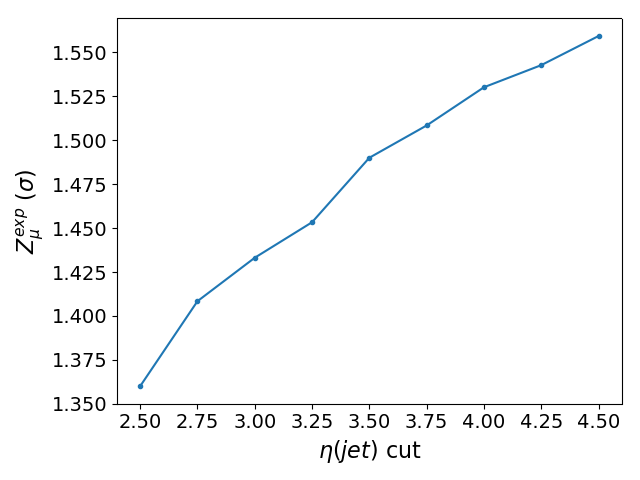
\includegraphics[width = 0.34\textwidth]{figures/signif_jetEta.png}
  	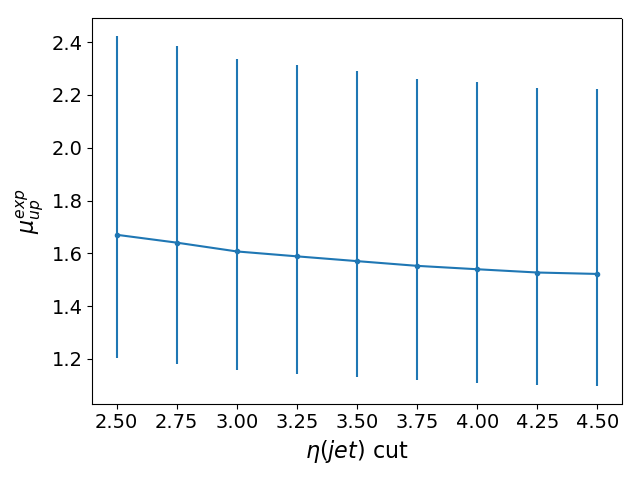
\includegraphics[width = 0.34\textwidth]{figures/exp_upper_jetEta.png}
  \centering
	\caption{\textbf{Left:} The expected significance ($Z_{\mu}^{exp}$) for different $\eta(jet)$ cuts is shown. The cuts applied on the $\eta(jet)$ are shown on the x-axis and the corresponding expected significance from the likelihood fit is shown on the y-axis. \textbf{Right:} Expected upper limit ($\mu_{up}^{exp}$) for different $\eta(jet)$ cuts is shown. The cuts applied on the $\eta(jet)$ are shown on the x-axis and corresponding expected upper limits are shown on the y-axis. Error bars representing the total uncertainty on the expected upper limits are shown as vertical lines.}
	\label{fig:4lep-jetEta-optimisation}
\end{figure}From Figure \ref{fig:4lep-jetEta-optimisation}, it can be seen that the $\eta(jet)$ cut which maximises the sensitivity of \tWZ in the tetralepton channel is requiring that $\eta(jet) < 4.5$. This selection criteria was set for the $\eta(jet)$ across all regions. In Figure \ref{fig:4lep-jetpt-optimisation} the expected significance ($Z_{\mu}^{exp}$) and expected upper limits ($\mu_{up}^{exp}$) for different $p_{T}(jet)$ cuts are shown.
\begin{figure}[h!]
	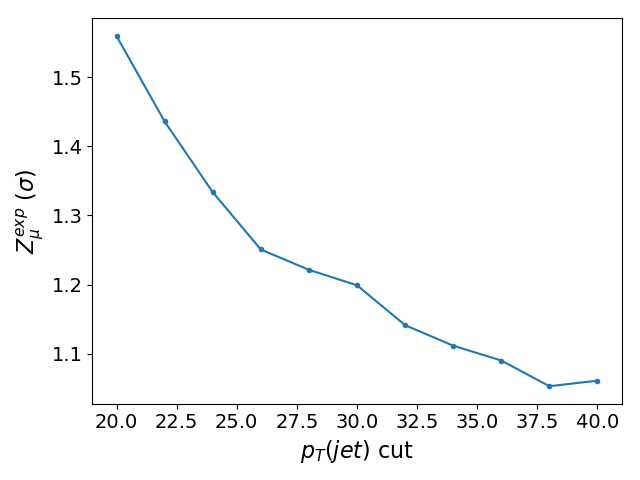
\includegraphics[width = 0.34\textwidth]{figures/signif_jetPt.png}
  	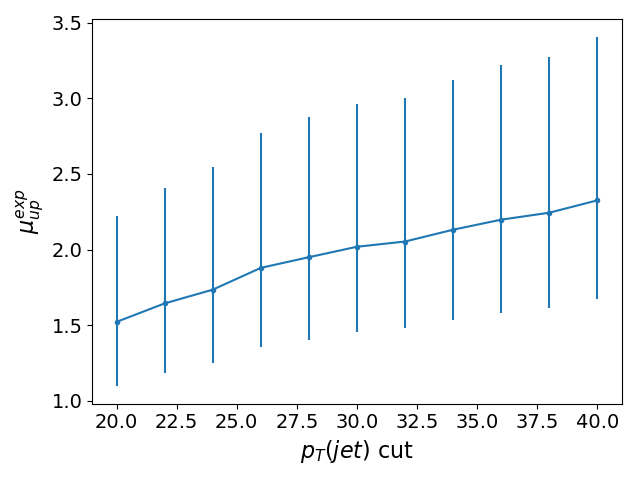
\includegraphics[width = 0.34\textwidth]{figures/exp_upper_jetPt.png}
  \centering
	\caption{\textbf{Left:} The expected significance ($Z_{\mu}^{exp}$) for different $p_{T}(jet)$ cuts is shown. The cuts applied on the $p_{T}(jet)$ are shown on the x-axis and the corresponding expected significance from the likelihood fit is shown on the y-axis. \textbf{Right:} Expected upper limit ($\mu_{up}^{exp}$) for different $p_{T}(jet)$ cuts is shown. The cuts applied on the $p_{T}(jet)$ are shown on the x-axis and corresponding expected upper limits are shown on the y-axis. Error bars representing the total uncertainty on the expected upper limits are shown as vertical lines.}
		\label{fig:4lep-jetpt-optimisation}
\end{figure}From Figure \ref{fig:4lep-jetpt-optimisation}, it can be seen that the $p_{T}(jet)$ cut which maximises the sensitivity of \tWZ is requiring that $p_{T}(jet) > 20$ GeV. This selection criteria was set for the $p_{T}(jet)$ across all regions. In Figure \ref{fig:4lep-btagWP-optimization} the expected significance ($Z_{\mu}^{exp}$) and expected upper limits ($\mu_{up}^{exp}$) for a range of different configurations of DL1r $b$-tagged jet working points across different regions.
\begin{figure}[h!]
	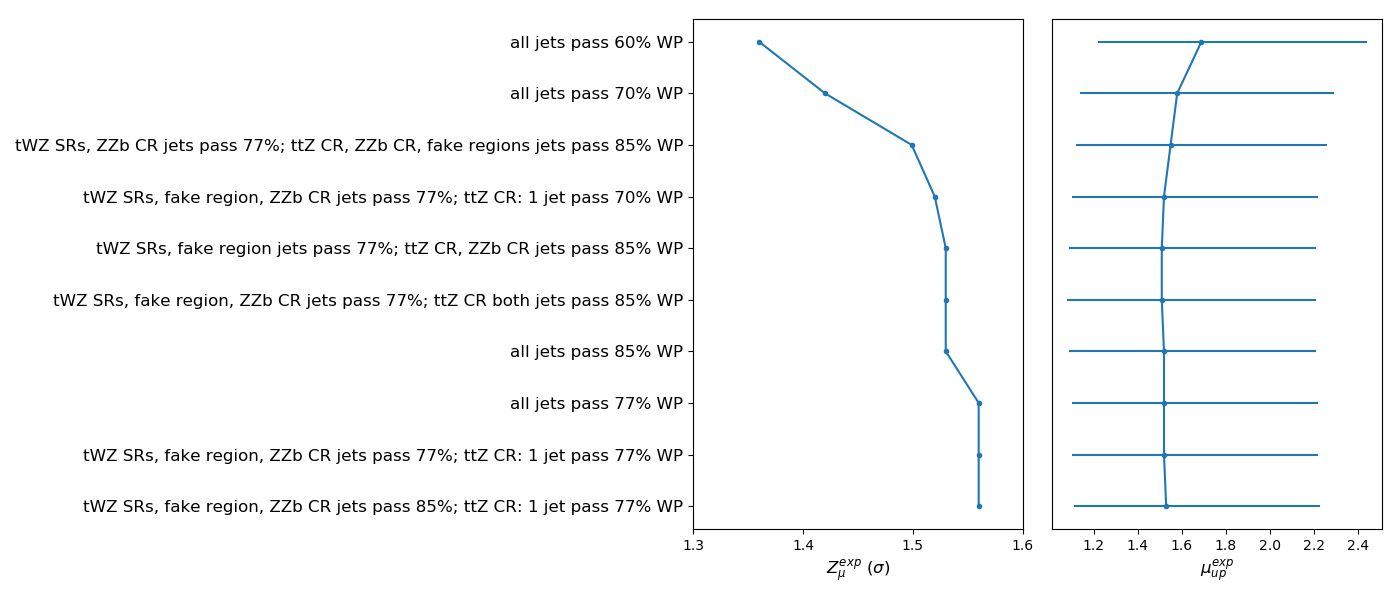
\includegraphics[width = 0.8\textwidth]{figures/btagWP_optimization.png}
  \centering
	\caption{Expected significance ($Z_{\mu}^{exp}$) and expected upper limit ($\mu_{up}^{exp}$) for different configurations of DL1r $b$-tagged jet working points is shown. The common y-axis shows the different configurations of DL1r $b$-tagged jet working points. On the left panel, the expected significance from the likelihood fit is shown on the x-axis. On the right panel, the expected upper limit from the likelihood fit is shown on the x-axis (with the corresponding total uncertainty represented by horizontal lines).}
	\label{fig:4lep-btagWP-optimization}
\end{figure}From Figure \ref{fig:4lep-btagWP-optimization}, it can be seen that requiring that $b$-tagged jets pass the 77$\%$ DL1r WP in the \tWZ SR, $(tWZ)_{\text{fake}}$ CR and the $ZZb$ CR and that at least one $b$-tagged jet in the $t\bar{t}Z$ SR passes the 77$\%$ DL1r WP (the other jet is just required to pass the 85$\%$ DL1r WP) maximises the sensitivity overall (compared to the other investigated configurations). This configuration was chosen $b$-tagged jets. The $p_{T}(\text{L Lepton})$ is constrained by the single lepton triggers \ref{tab:triggers}. A cut was chosen to be applied on the $p_{T}(\text{NL Lepton})$ slightly tighter than the tightest single lepton $p_{T}$ cut in the trigger. The $p_{T}(\text{NL Lepton})$ cut can be optimized by comparing the expected significance and limit for a range of $p_{T}{(\text{NL Lepton})}$ cuts to determine the cut which maximizes sensitivity. In Figure \ref{fig:4lep-NLlep-optimization} the expected significance ($Z_{\mu}^{exp}$) and expected upper limits ($\mu_{up}^{exp}$) for different $p_{T}(\text{NL Lepton})$ cuts is shown.
\begin{figure}[h!]
	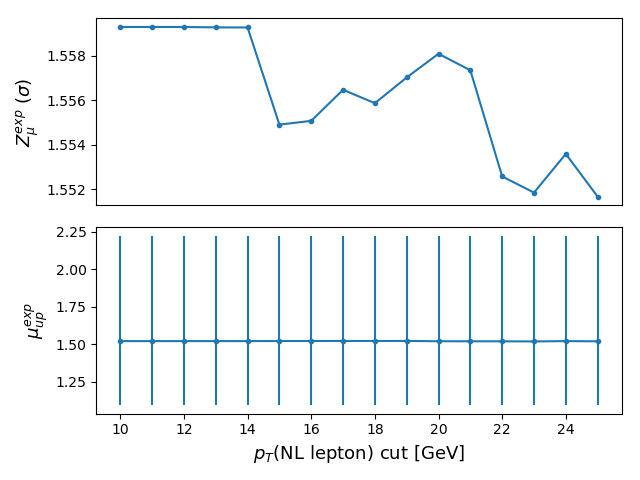
\includegraphics[width = 0.55\textwidth]{figures/NL_Lep_optimization.png}
  \centering
	\caption{Expected significance ($Z_{\mu}^{exp}$) and expected upper limit ($\mu_{up}^{exp}$) for different $p_{T}(\text{NL Lepton})$ cuts is shown. The common x-axis shows cut applied to the $p_{T}$ of the next-to-leading lepton. On the top panel, the expected significance from the likelihood fit is shown on the y-axis. On the bottom panel, the expected upper limit from the likelihood fit is shown on the y-axis (with the corresponding total uncertainty represented by vertical lines).}
	\label{fig:4lep-NLlep-optimization}
\end{figure}Since there is a very small change between the different $p_{T}(\text{NL Lepton})$ cuts on the sensitivity of \tWZ, a $p_{T}(\text{NL Lepton})$ cut is applied at 18 GeV (avoiding a $p_{T}$ cut near the sharp drop in expected significance after 28 GeV), therefore applying a cut above the tightest, looser dilepton trigger $p_{T}$ cut (17 GeV) to suppress any systematic from the modelling of the trigger efficiency.

\section{Signal and Control Regions}
\label{sec:sig-and-control-regions}
In this section, expected number of events of variables in each region are shown. For each figure in this section, the data is given by the black points and the MC predictions for each process are given by the filled histograms. The vertical lines on the data points represent the statistical uncertainty in the data and the diagonally-lined bands represent the total (statistical and systematic added in quadrature) uncertainty. The lower panel in each plot shows the ratios of the data to the theoretical predictions. In order to suppress a bias towards large signal observations in the development of the analysis, data has not been analysed in bins where the expected $\frac{signal}{background}$ exceeds 0.1. This is known as blinding. Blinded bins are shaded with black diagonal lines and their data points are omitted. In Table \ref{tab:4Lep-PreFit-Yields}, the expected number of events for each sample in each region are shown.
\begin{table}[h!]
    \resizebox{1\textwidth}{!}{%
\begin{tabular}{|ll|l|l|l|l|l|}
\hline
\multicolumn{2}{|l|}{}                                      & $tWZ$ OF SR                      & $tWZ$ SF SR                    & $t\bar{t}Z$ CR                      & $ZZb$ CR                      & $(tWZ)_{\text{fake}}$ CR       \\ \hline
\multicolumn{2}{|l|}{$t\bar{t}Z$}                                   & 13.9 $\pm$ 1.8         & 10.1 $\pm$ 1.4       & 31.7 $\pm$ 4.5      & 5.3 $\pm$ 0.7      & 19.1 $\pm$ 2.5      \\
\multicolumn{2}{|l|}{$t\bar{t}Z$ fakes}                             & 0.068 $\pm$ 0.048    & 0.032 $\pm$ 0.026    & 0.07 $\pm$ 0.04   & 0.05 $\pm$ 0.03   & 5.0 $\pm$ 2.5     \\
\multicolumn{2}{|l|}{$tWZ$}                                   & 3.8 $\pm$ 0.4       & 2.6 $\pm$ 0.3     & 2.6 $\pm$ 0.9     & 1.4 $\pm$ 0.2      & 5.0 $\pm$ 0.7     \\
\multicolumn{2}{|l|}{$ZZ$}                                    & 0.5 $\pm$ 0.2       & 8.8 $\pm$ 2.7      & 1.2 $\pm$ 0.4     & 46 $\pm$ 14      & 7.8 $\pm$ 2.4      \\ \hline
\multicolumn{1}{|l|}{\multirow{9}{*}{other}} & $t\bar{t}$           & 6e-06 $\pm$ 3e-06       & 0.25 $\pm$ 0.44      & 0.27 $\pm$ 0.22    & 6e-06 $\pm$ 3e-06     & 2.4 $\pm$ 0.9     \\
\multicolumn{1}{|l|}{}                       & $tZq$          & 0.08 $\pm$ 0.04     & 0.08 $\pm$ 0.04   & 0.06 $\pm$ 0.03  & 0.06 $\pm$ 0.02   & 4.9 $\pm$ 0.8     \\
\multicolumn{1}{|l|}{}                       & $t\bar{t}W$ & 0.007 $\pm$ 0.007  & 0.003 $\pm$ 0.003 & 6e-06 $\pm$ 3e-06    & 0.002 $\pm$ 0.006 &1.0 $\pm$ 0.3   \\
\multicolumn{1}{|l|}{}                       & $WZ$        & 0.04 $\pm$ 0.02     & 0.04 $\pm$ 0.02   & 0.013 $\pm$ 0.013  & 0.05 $\pm$ 0.03  & 1.8 $\pm$ 0.4     \\
\multicolumn{1}{|l|}{}                       & $t\bar{t}t$          & 0.0010 $\pm$ 0.0008 & 0.002 $\pm$ 0.001 & 0.014 $\pm$ 0.004 & 6e-06 $\pm$ 3e-06     & 0.010 $\pm$ 0.004 \\
\multicolumn{1}{|l|}{}                       & $t\bar{t}t\bar{t}$         & 0.0093 $\pm$ 0.0081    & 0.011 $\pm$ 0.009 & 0.057 $\pm$ 0.021  & 6e-06 $\pm$ 3e-06     & 0.02 $\pm$ 0.01 \\
\multicolumn{1}{|l|}{}                       & $t\bar{t}WW$         & 0.029 $\pm$ 0.026     & 0.03 $\pm$ 0.02   & 0.26 $\pm$ 0.10    & 0.01 $\pm$ 0.03    & 0.20 $\pm$ 0.06   \\
\multicolumn{1}{|l|}{}                       & $VVV (V = W/Z)$           & 0.28 $\pm$ 0.09     & 0.20 $\pm$ 0.06    & 0.07 $\pm$ 0.02  & 0.20 $\pm$ 0.05   & 0.3 $\pm$ 0.1   \\
\multicolumn{1}{|l|}{}                       & $t\bar{t}H$          & 0.85 $\pm$ 0.18       & 0.67 $\pm$ 0.14     & 2.0 $\pm$ 0.4     & 0.15 $\pm$ 0.04    & 2.2 $\pm$ 0.5      \\ \hline
                                             & Total        & 19.7 $\pm$ 2.0         & 22.9 $\pm$ 3.1       & 38.4 $\pm$ 4.6       & 53.2 $\pm$ 14.0       & 49.5 $\pm$ 4.8      \\ \hline
                                             & data         & -                                         & -                                       & 36                                      & 49                                       & 57                                      \\ \hline
\end{tabular}}
\caption{The expected number of events for each sample in each region is shown.}
\label{tab:4Lep-PreFit-Yields}
\end{table}The finite number of events expected to be observed in data (MC simulation) carries an associated statistical uncertainty. To first order, this uncertainty can be written as the square root of the expected number of events to be observed in data. In contrast to this, predictions based on MC simulation carry uncertainties due to the finite number of simulated events utilised. This uncertainty can be quantified by the Number of Equivalent Events~\cite{N_equiv_Derivation}, $N_{equiv}$, which relates the sample of $N$ events (weighted by MC event weights) to $N_{equiv}$ events with all MC event weights equal to 1, that would have the same relative statistical fluctuation. The Number of Equivalent Events, $N_{equiv}$, can be written as,
\begin{equation}
N_{equiv} = \frac{ (\sum_{i}^{N} w_{i})^2  }{\sum_{i}^{N} w_i^2 }
\end{equation}
where $w_i$ is the MC event weight for event $i$. The standard uncertainty of $N_{equiv}$ is given by $u(N_{equiv}) = \sqrt{N_{equiv}}$. The Number of Equivalent Events for each sample in each region can be studied in order to ensure that the number of events simulated for a given process is large in comparison to the number of events expected for that process in data, thereby ensuring that uncertainties from MC statistics will be small (or sub-leading). In Table \ref{tab:N-equiv}, the number of equivalent events, $N_{equiv}$, is shown for each sample in each region. 
\begin{table}[h!]	
\resizebox{0.9\textwidth}{!}{%
\begin{tabular}{|l|l|l|l|l|l|} 
\hline
                  & $tWZ$ OF SR   & $tWZ$ SF SR   & $t\bar{t}Z$ CR & $ZZb$ CR        & $(tWZ)_{\text{fake}}$ CR  \\ 
\hline
                  & $N_{equiv}$   & $N_{equiv}$   & $N_{equiv}$    & $N_{equiv}$     & $N_{equiv}$               \\ 
\hline
$tWZ$             & 6463 $\pm$ 80 & 4153 $\pm$ 64 & 4800 $\pm$ 69  & 2497 $\pm$ 50   & 8645 $\pm$ 93             \\
$t\bar{t}Z$       & 1364 $\pm$ 37 & 1031 $\pm$ 32 & 3237 $\pm$ 57  & 561 $\pm$ 24    & 1923 $\pm$ 44             \\
$ZZ$              & 51 $\pm$ 7    & 975 $\pm$ 31  & 268 $\pm$ 16   & 7023 $\pm$ 84   & 969 $\pm$ 31              \\
other             & 748 $\pm$ 27  & 2.5 $\pm$ 1.6 & 4.2 $\pm$ 2.1  & 255 $\pm$ 16    & 21.5 $\pm$ 4.6            \\
$t\bar{t}Z$ fakes & 6.7 $\pm$ 2.6 & 1.3 $\pm$ 1.1 & 16.1 $\pm$ 4.0 & 7.2 $\pm$ 2.7   & 484 $\pm$ 22              \\ 
\hline
Total             & 8633 $\pm$ 93 & 6163 $\pm$ 79 & 8326 $\pm$ 91  & 10344 $\pm$ 102 & 12044 $\pm$ 110           \\
\hline
\end{tabular}}
\centering
\caption{The number of equivalent events, $N_{equiv}$, is shown for each sample in each region.}
\label{tab:N-equiv}
\end{table}$N_{equiv}$ is much larger compared to the number of expected events (See Table \ref{tab:4Lep-PreFit-Yields}) for the signal and background processes in all regions. This tells us that there is a large number of simulated events for these samples. Therefore ensuring that uncertainties resulting from MC statistics will be small (or sub-leading).

\subsection{$tWZ$ OF SR}
\label{sec:controlplotstetralepton-tWZ-OF-SR}

%%%%%%%%%%%%%%%%%%%%%%%%%%%%%%%%%%%%
%%%%%%%%%%%%%%%%%%%%%%%%%%%%%%%%%%%%
%%%%%%%      tWZ OF region   %%%%%%%%%%
%%%%%%%%%%%%%%%%%%%%%%%%%%%%%%%%%%%%
%%%%%%%%%%%%%%%%%%%%%%%%%%%%%%%%%%%%

In this section, comparisons of simulation and data for different variables in the $tWZ$ OF SR are shown. In Figure \ref{fig:4lep-OF-SR-leptonPlots}, comparisons of simulation and data for $p_{T}$, $\eta$ and $\phi$ for leading (L) leptons and leading (NL) jets in the $tWZ$ OF SR are shown.
\begin{figure}[htbp]
\centering
  \begin{tabular}{ccc}

    %%%%%%%%%%%%%%%
    %%% Leptons %%%
    %%%%%%%%%%%%%%%

    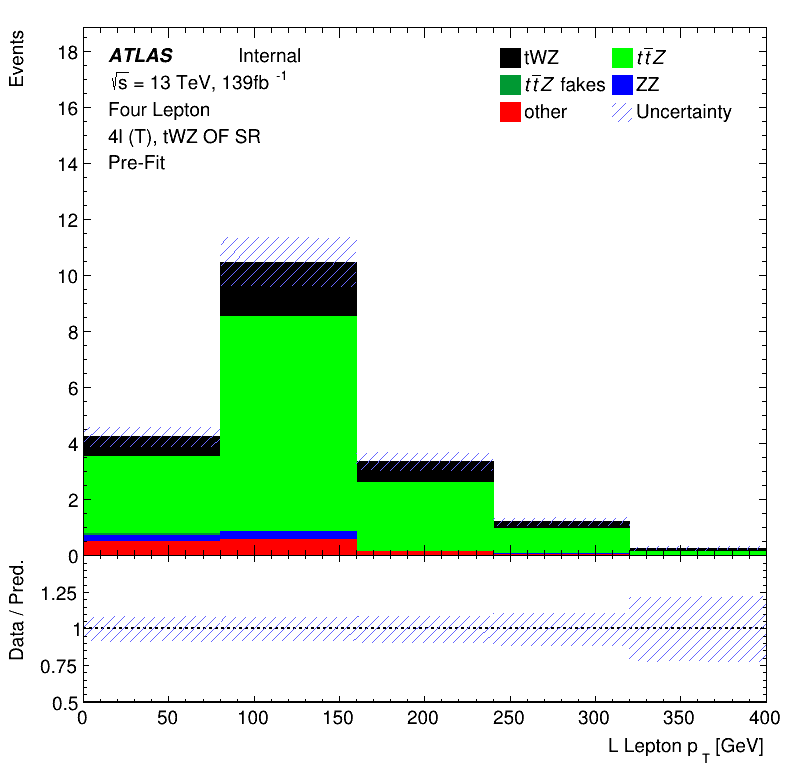
\includegraphics[width=.25\textwidth]{figures/PreFitPlots/lep4_tWZ_4T_OF_L_lepton_pt.png} &
    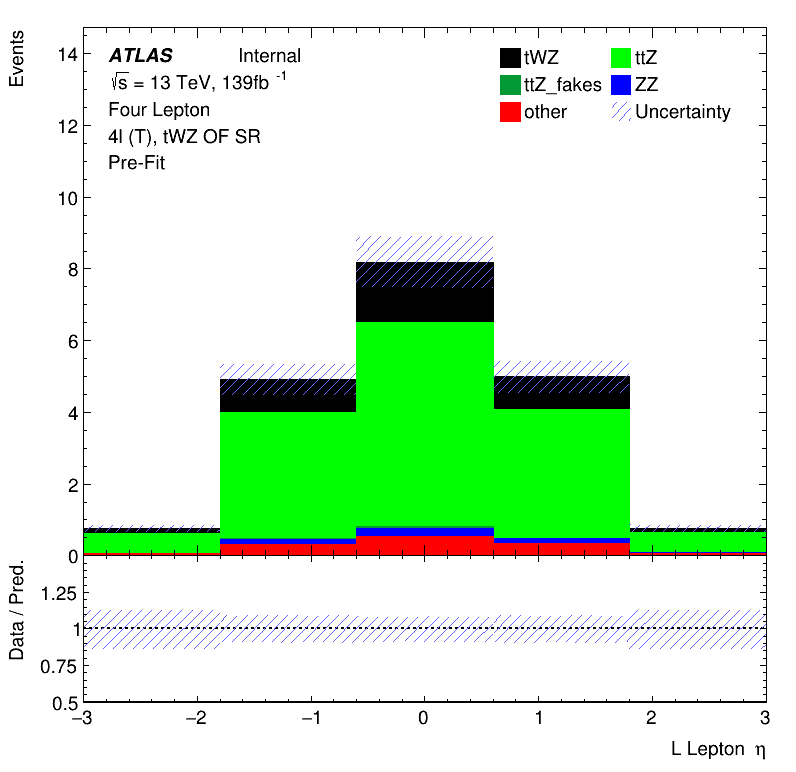
\includegraphics[width=.25\textwidth]{figures/PreFitPlots/lep4_tWZ_4T_OF_L_lepton_eta.png} &
    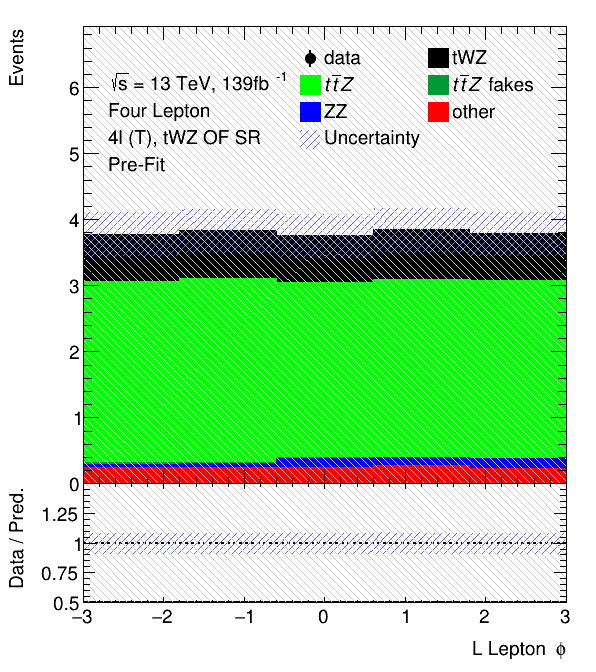
\includegraphics[width=.25\textwidth]{figures/PreFitPlots/lep4_tWZ_4T_OF_L_lepton_phi.png} \\
    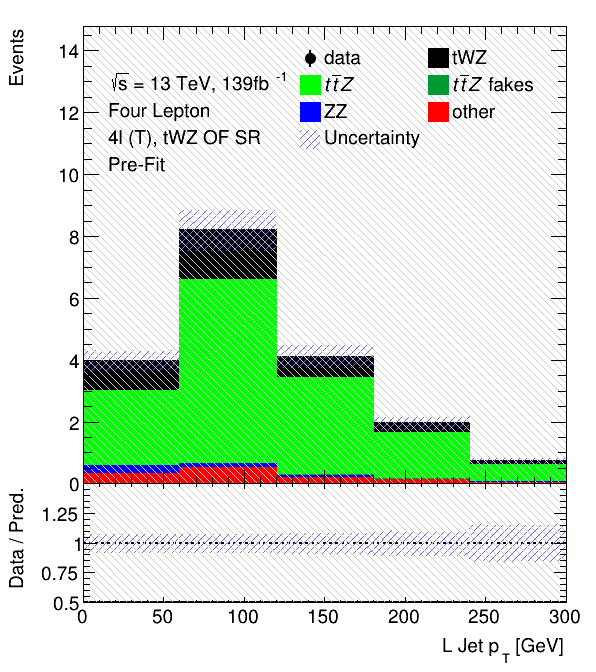
\includegraphics[width=.25\textwidth]{figures/PreFitPlots/lep4_tWZ_4T_OF_LJet_pt.png} &
    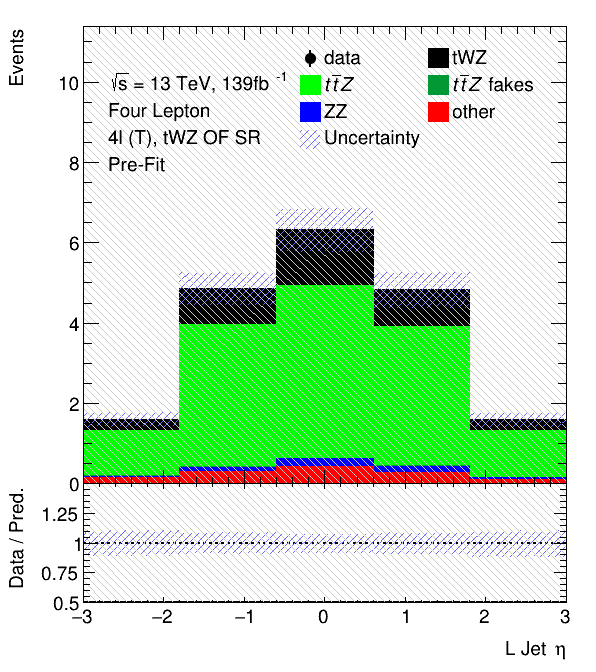
\includegraphics[width=.25\textwidth]{figures/PreFitPlots/lep4_tWZ_4T_OF_LJet_eta.png} &
    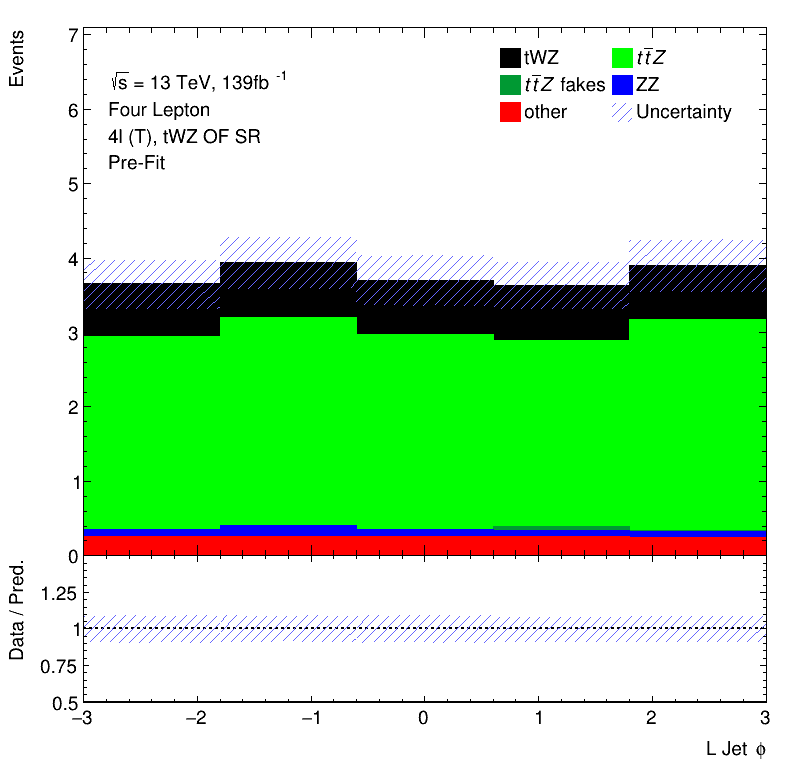
\includegraphics[width=.25\textwidth]{figures/PreFitPlots/lep4_tWZ_4T_OF_LJet_phi.png} \\

  \end{tabular}
    \caption{Comparisons of simulation and data of $p_{T}$, $\eta$ and $\phi$ for leading (L) leptons (top row) and leading (NL) jets (bottom row) in the $tWZ$ OF SR are shown.}\label{fig:4lep-OF-SR-leptonPlots}
\end{figure}The bins in all of the plots in Figure \ref{fig:4lep-OF-SR-leptonPlots} have $\frac{signal}{background}$ exceeding 0.1. This region is enriched in $tWZ$ signal events. In Figure \ref{fig:4lep-OF-SR-jets-bjet}, comparisons of simulation and data of $H_{T}$ (scalar sum of Jet $p_{T}$), the Number of jets, the scalar sum of $b$-tagged jet $p_{T}$ and the number of $b$-tagged jets in the $tWZ$ OF SR are shown.
\begin{figure}[htbp]
 \centering

    %%%%%%%%%%%%%%%%%
    %%%%% jets %%%%%
    %%%%%%%%%%%%%%%%%

    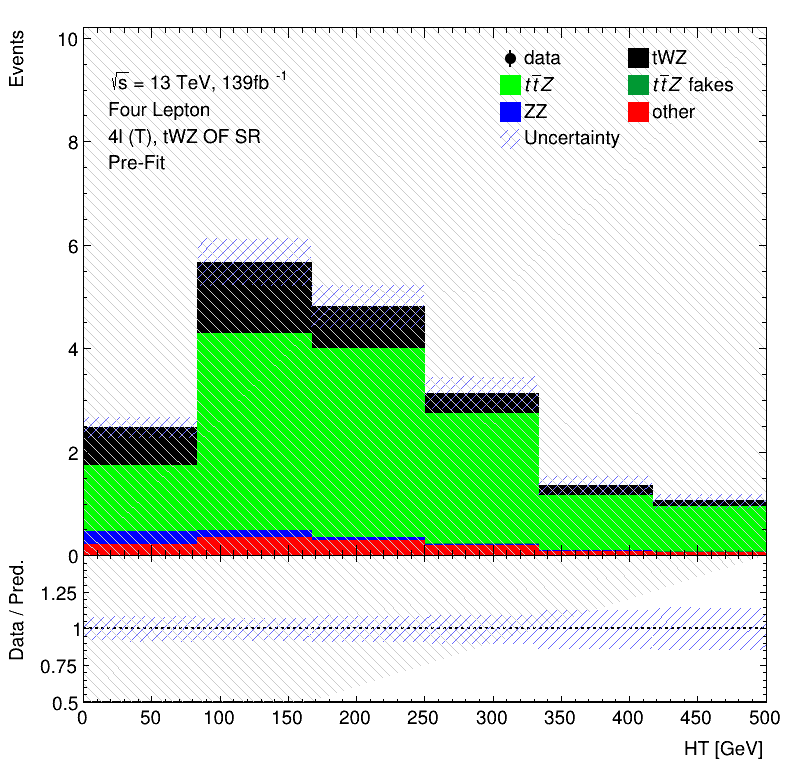
\includegraphics[width=.25\textwidth]{figures/PreFitPlots/lep4_tWZ_4T_OF_HT.png}   \quad
    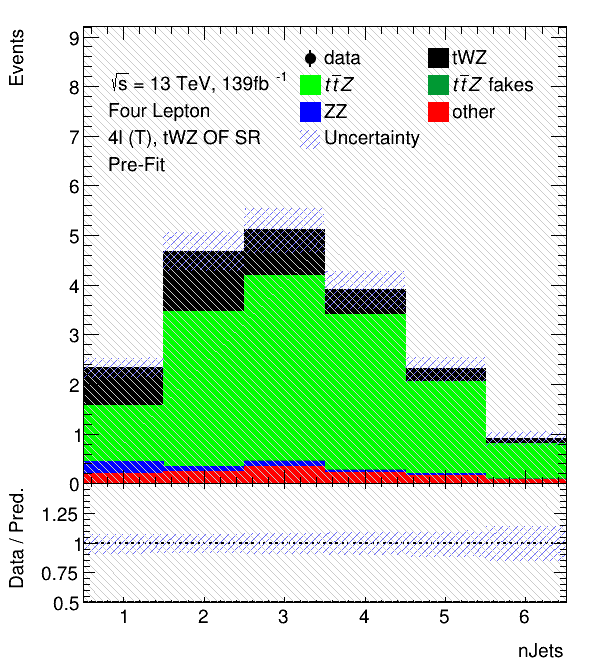
\includegraphics[width=.25\textwidth]{figures/PreFitPlots/lep4_tWZ_4T_OF_Num_Jets.png}
	
	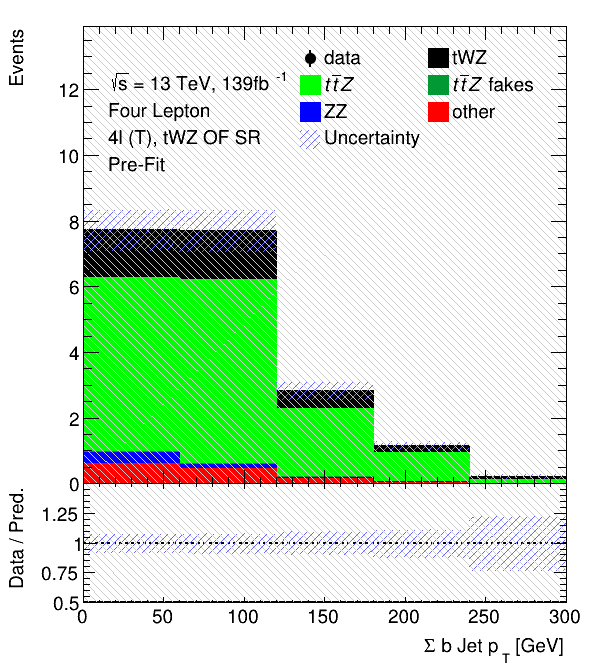
\includegraphics[width=.25\textwidth]{figures/PreFitPlots/lep4_tWZ_4T_OF_sum_bJet_Pt.png}  \quad
    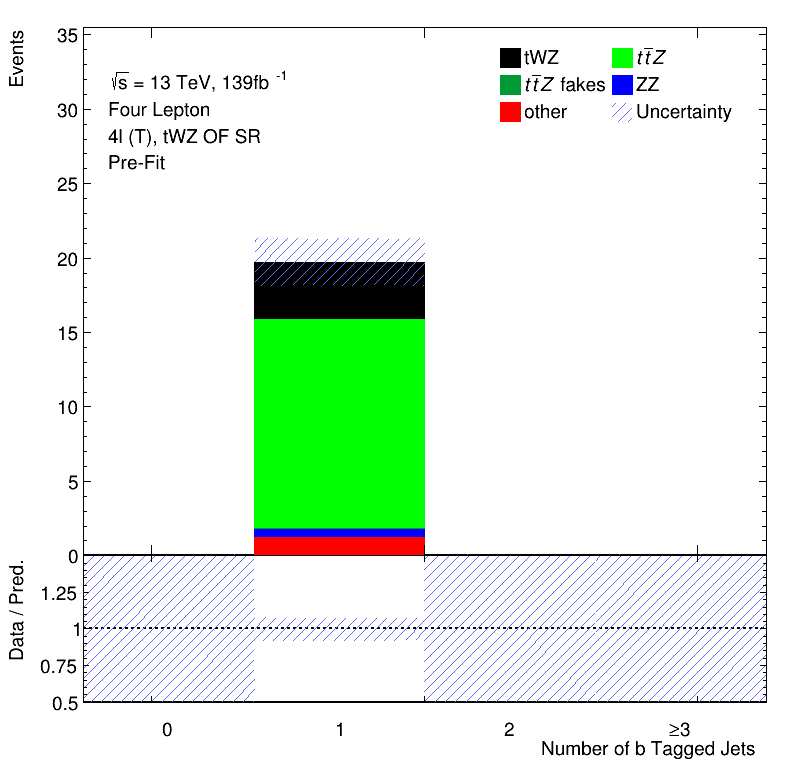
\includegraphics[width=.25\textwidth]{figures/PreFitPlots/lep4_tWZ_4T_OF_Num_bJets.png}

\caption{Comparisons of simulation and data of $H_{T}$ (scalar sum of Jet $p_{T}$), the Number of jets, the scalar sum of $b$-tagged jet $p_{T}$ and the number of $b$-tagged jets (top left to bottom right) in the $tWZ$ OF SR are shown.}\label{fig:4lep-OF-SR-jets-bjet} 
\end{figure}All bins for each plot in Figure \ref{fig:4lep-OF-SR-jets-bjet} have $\frac{signal}{background}$ exceeding 0.1 and are therefore blinded. This region is therefore enriched in $tWZ$ signal events.

\subsection{$tWZ$ SF SR}
\label{sec:controlplotstetralepton-tWZ-SF-SR}

%%%%%%%%%%%%%%%%%%%%%%%%%%%%%%%%%%%%
%%%%%%%%%%%%%%%%%%%%%%%%%%%%%%%%%%%%
%%%%%%%      tWZ SF region   %%%%%%%%%%
%%%%%%%%%%%%%%%%%%%%%%%%%%%%%%%%%%%%
%%%%%%%%%%%%%%%%%%%%%%%%%%%%%%%%%%%%

In this section, expected number of events of variables in the $tWZ$ SF SR are shown. In Figure \ref{fig:4lep-SF-SR-leptonPlots}, comparisons of simulation and data of $p_{T}$, $\eta$ and $\phi$ for leading (L) leptons and leading (NL) jets in the $tWZ$ SF SR are shown.
\begin{figure}[htbp]
\centering
  \begin{tabular}{ccc}

    %%%%%%%%%%%%%%%
    %%% Leptons %%%
    %%%%%%%%%%%%%%%

    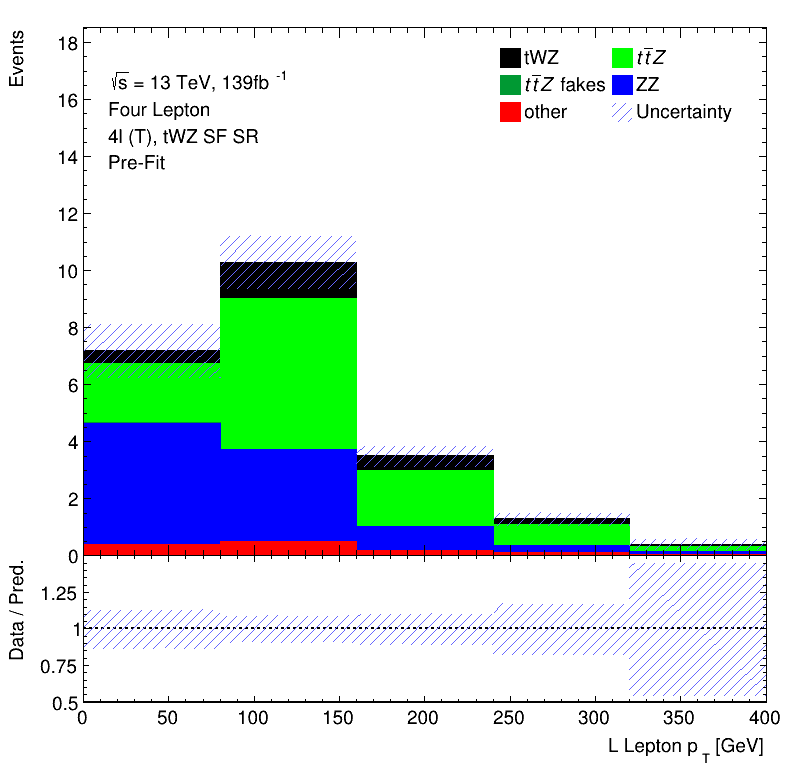
\includegraphics[width=.25\textwidth]{figures/PreFitPlots/lep4_tWZ_4T_SF_L_lepton_pt.png} &
    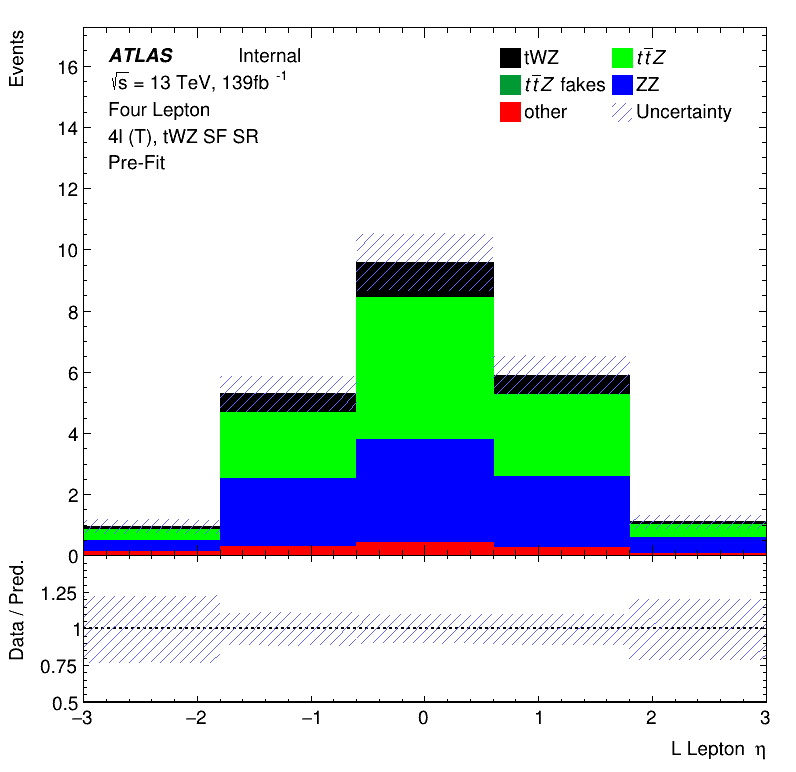
\includegraphics[width=.25\textwidth]{figures/PreFitPlots/lep4_tWZ_4T_SF_L_lepton_eta.png} &
    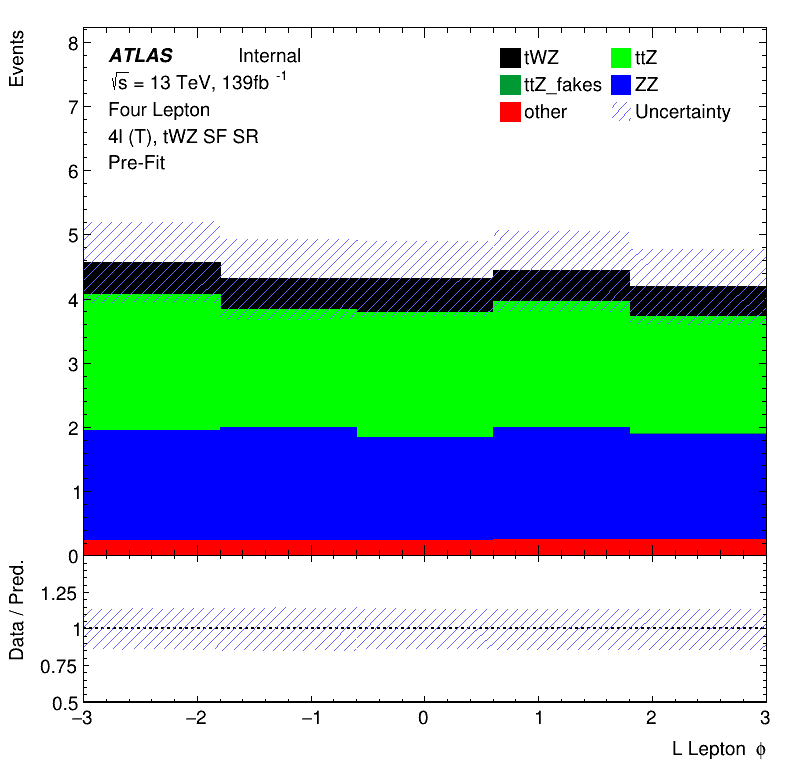
\includegraphics[width=.25\textwidth]{figures/PreFitPlots/lep4_tWZ_4T_SF_L_lepton_phi.png} \\
    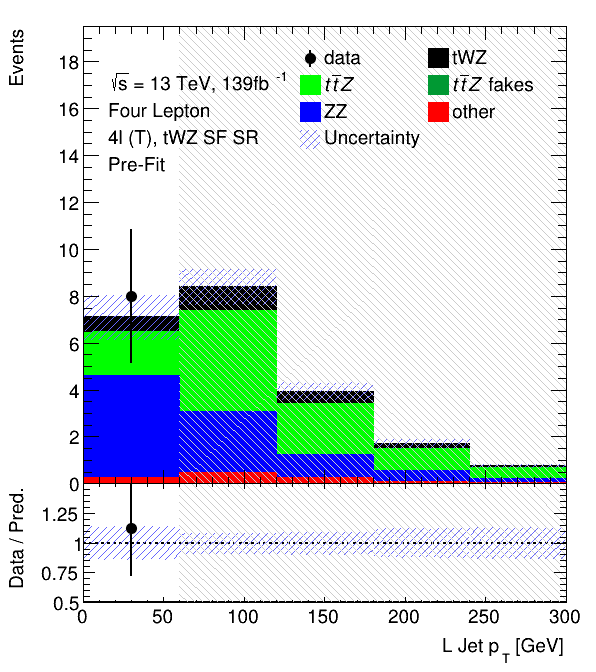
\includegraphics[width=.25\textwidth]{figures/PreFitPlots/lep4_tWZ_4T_SF_LJet_pt.png} &
    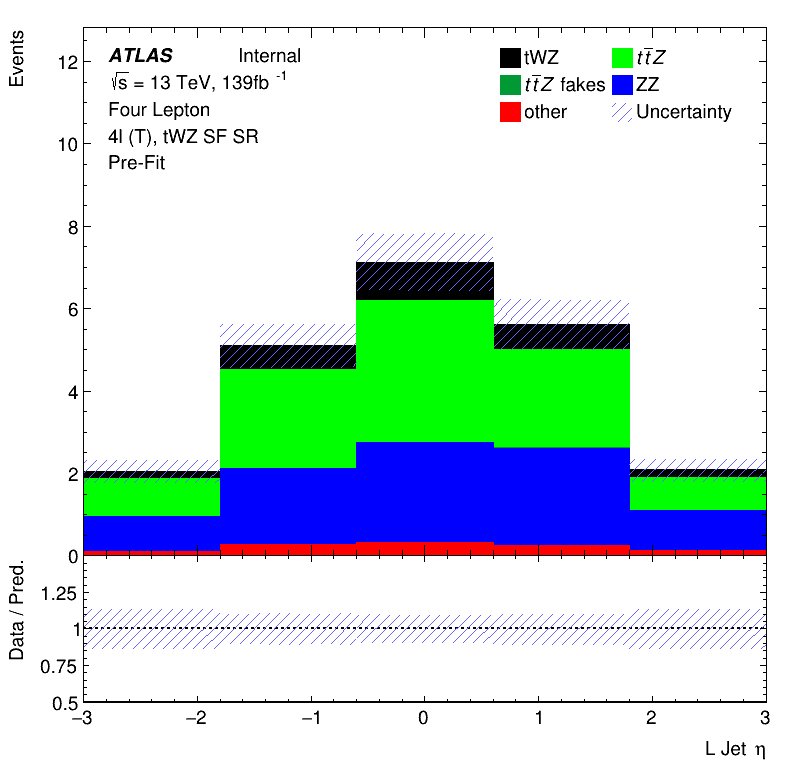
\includegraphics[width=.25\textwidth]{figures/PreFitPlots/lep4_tWZ_4T_SF_LJet_eta.png} &
    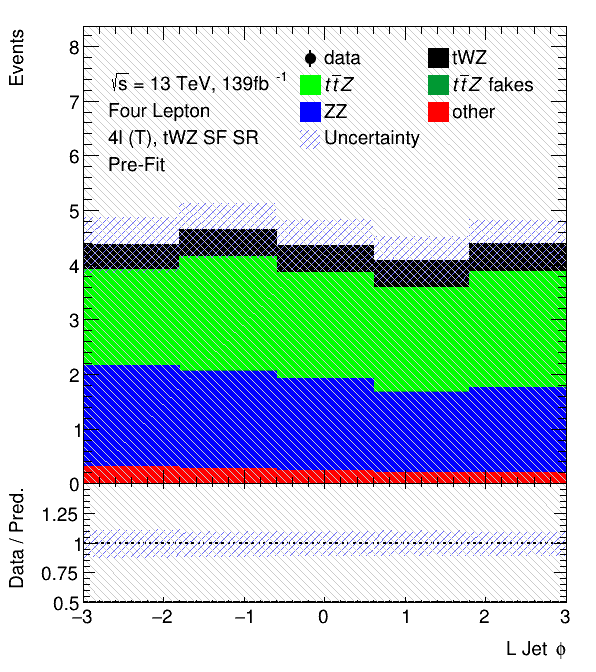
\includegraphics[width=.25\textwidth]{figures/PreFitPlots/lep4_tWZ_4T_SF_LJet_phi.png} \\

  \end{tabular}
    \caption{Comparisons of simulation and data of $p_{T}$, $\eta$ and $\phi$ for leading (L) leptons (top row) and leading (NL) jets (bottom row) in the $tWZ$ SF SR are shown.}
  \label{fig:4lep-SF-SR-leptonPlots}
\end{figure}The vast majority of bins for each plot in Figure \ref{fig:4lep-SF-SR-leptonPlots} have $\frac{signal}{background}$ exceeding 0.1 and are therefore blinded. This region is therefore enriched in $tWZ$ signal events. In Figure \ref{fig:4lep-SF-SR-jets-bjet}, comparisons of simulation and data of $H_{T}$ (scalar sum of Jet $p_{T}$), the Number of jets, the scalar sum of $b$-tagged jet $p_{T}$ and the number of $b$-tagged jets in the $tWZ$ SF SR are shown.
\begin{figure}[htbp]
 \centering

    %%%%%%%%%%%%%%%%%
    %%%%% jets %%%%%
    %%%%%%%%%%%%%%%%%

    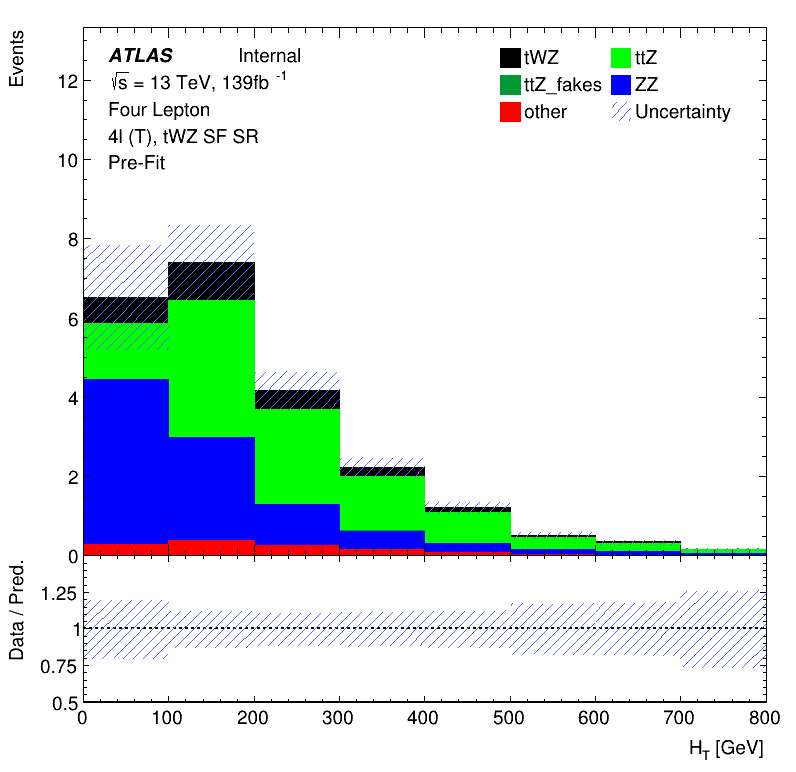
\includegraphics[width=.25\textwidth]{figures/PreFitPlots/lep4_tWZ_4T_SF_HT.png}   \quad
    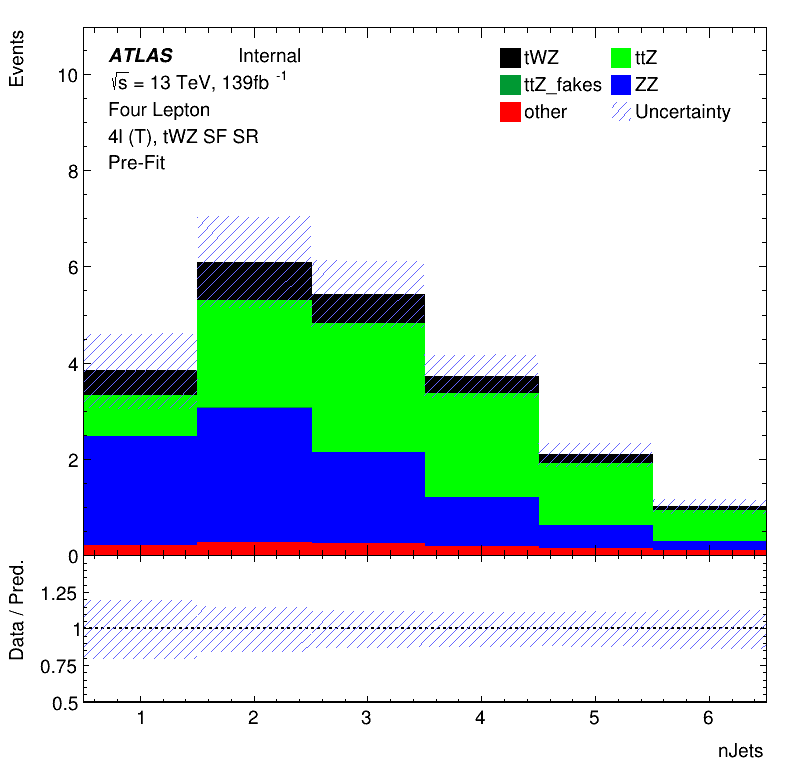
\includegraphics[width=.25\textwidth]{figures/PreFitPlots/lep4_tWZ_4T_SF_Num_Jets.png}
	
	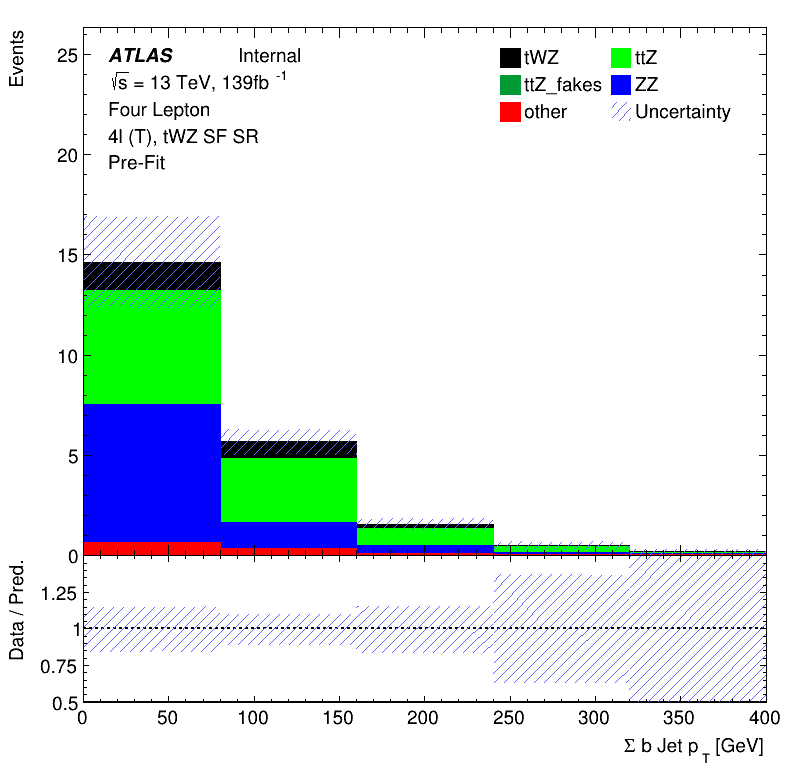
\includegraphics[width=.25\textwidth]{figures/PreFitPlots/lep4_tWZ_4T_SF_sum_bJet_Pt.png}  \quad
    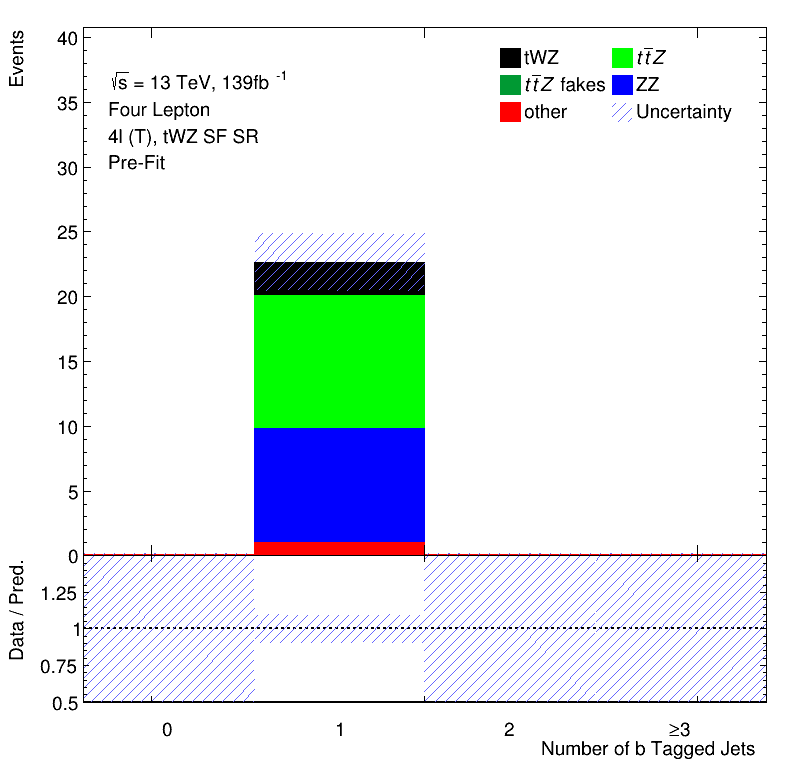
\includegraphics[width=.25\textwidth]{figures/PreFitPlots/lep4_tWZ_4T_SF_Num_bJets.png}

\caption{Comparisons of simulation and data of $H_{T}$ (scalar sum of Jet $p_{T}$), the Number of jets, the scalar sum of $b$-tagged jet $p_{T}$ and the number of $b$-tagged jets (top left to bottom right) in the $tWZ$ SF SR are shown.}\label{fig:4lep-SF-SR-jets-bjet} 
\end{figure}The vast majority of bins in each plot in Figure \ref{fig:4lep-SF-SR-jets-bjet} have $\frac{signal}{background}$ exceeding 0.1 and are therefore blinded. This region is therefore enriched in $tWZ$ signal events. The deviations in data and simulation in the two bins (in the $HT$ and $\sigma b$ jet $p_{T}$ distributions) which are not blinded, are within the expected uncertainties.


\subsection{$t\bar{t}Z$ CR}
\label{sec:controlplotstetralepton-ttZ-CR}

%%%%%%%%%%%%%%%%%%%%%%%%%%%%%%%%%%%%
%%%%%%%%%%%%%%%%%%%%%%%%%%%%%%%%%%%%
%%%%%%%      ttZ CR   %%%%%%%%%%
%%%%%%%%%%%%%%%%%%%%%%%%%%%%%%%%%%%%
%%%%%%%%%%%%%%%%%%%%%%%%%%%%%%%%%%%%

In this section, expected number of events of variables in the $t\bar{t}Z$ CR are shown. In Figure \ref{fig:4lep-ttZ-CR-leptonPlots}, comparisons of simulation and data of $p_{T}$, $\eta$ and $\phi$ for leading (L) leptons and leading (NL) jets in the $t\bar{t}Z$ CR are shown.
\begin{figure}[htbp]
\centering
  \begin{tabular}{ccc}

    %%%%%%%%%%%%%%%
    %%% Leptons %%%
    %%%%%%%%%%%%%%%

    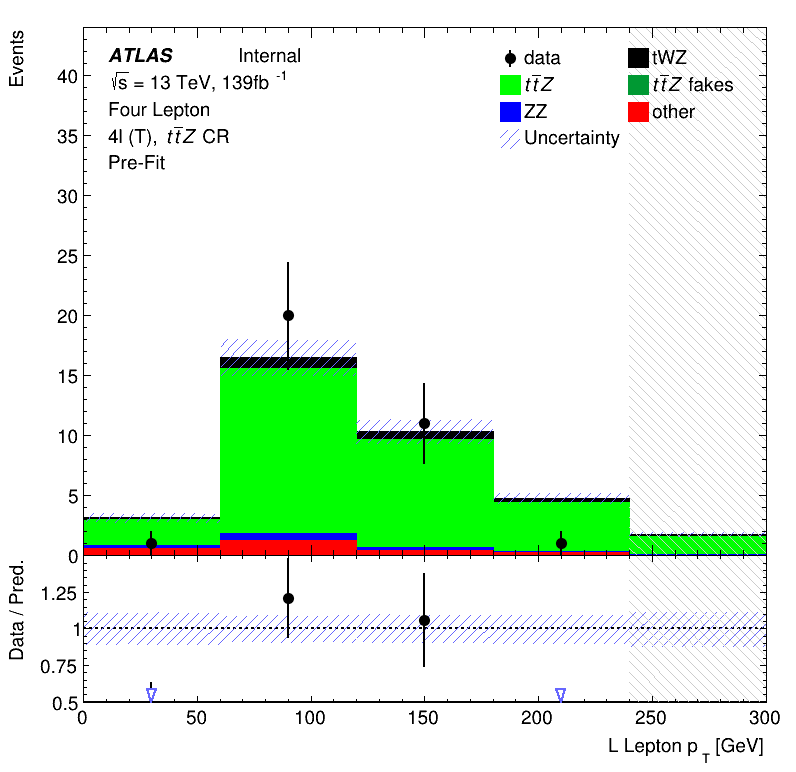
\includegraphics[width=.25\textwidth]{figures/PreFitPlots/lep4_ttZ_4T_L_lepton_pt.png} &
    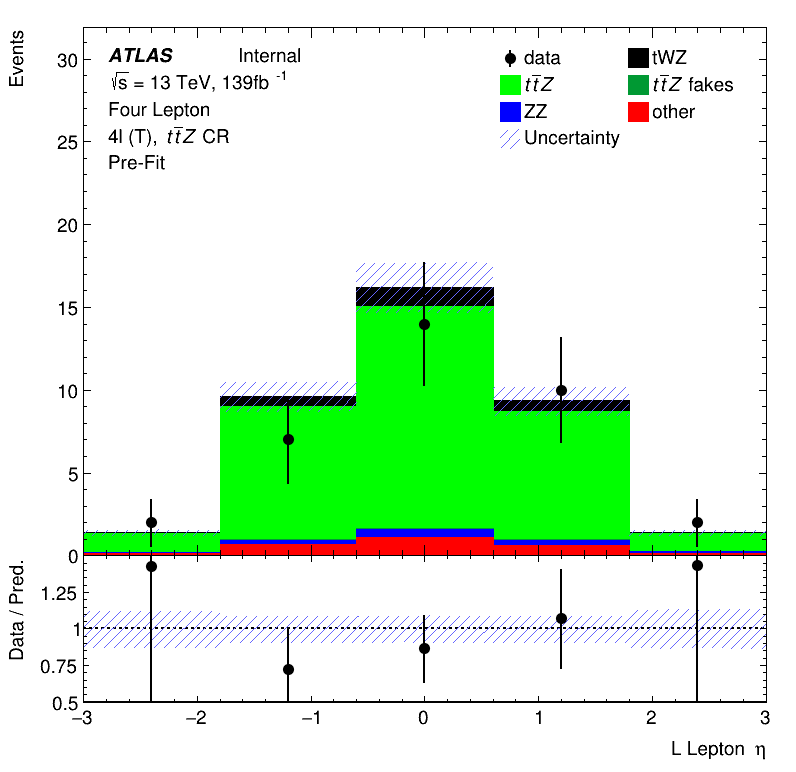
\includegraphics[width=.25\textwidth]{figures/PreFitPlots/lep4_ttZ_4T_L_lepton_eta.png} &
    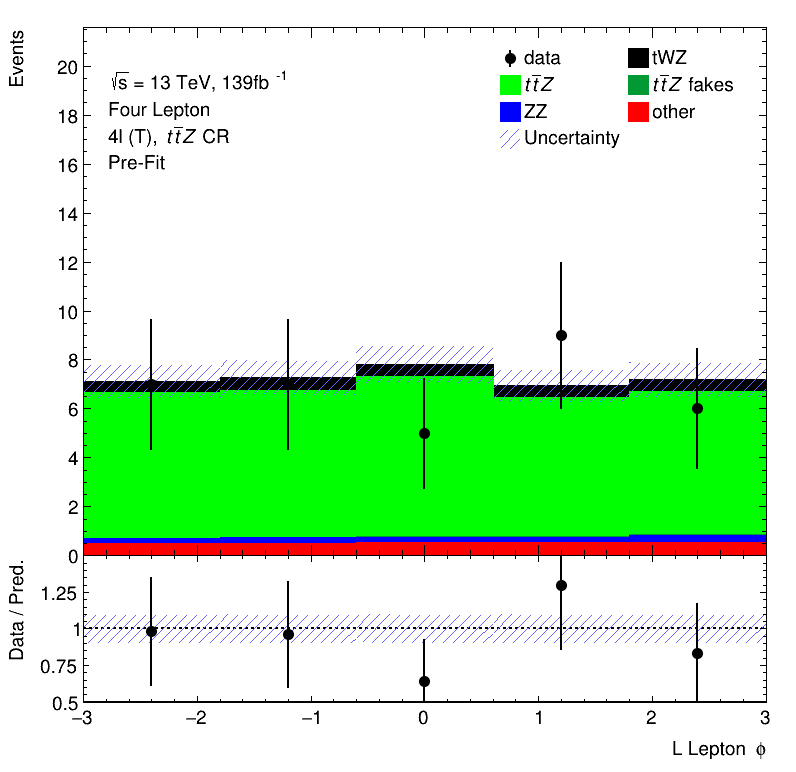
\includegraphics[width=.25\textwidth]{figures/PreFitPlots/lep4_ttZ_4T_L_lepton_phi.png} \\
    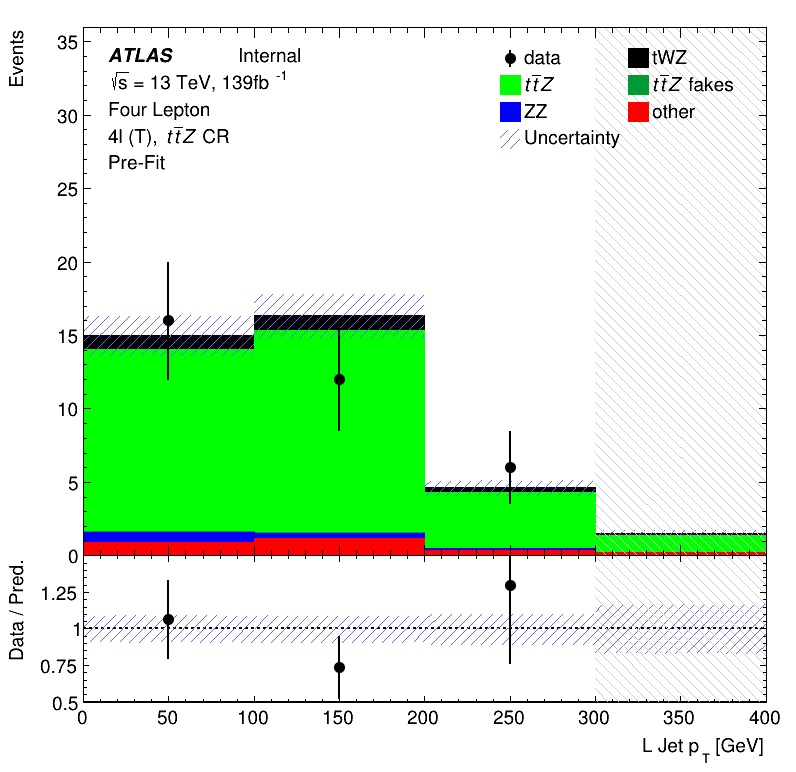
\includegraphics[width=.25\textwidth]{figures/PreFitPlots/lep4_ttZ_4T_LJet_pt.png} &
    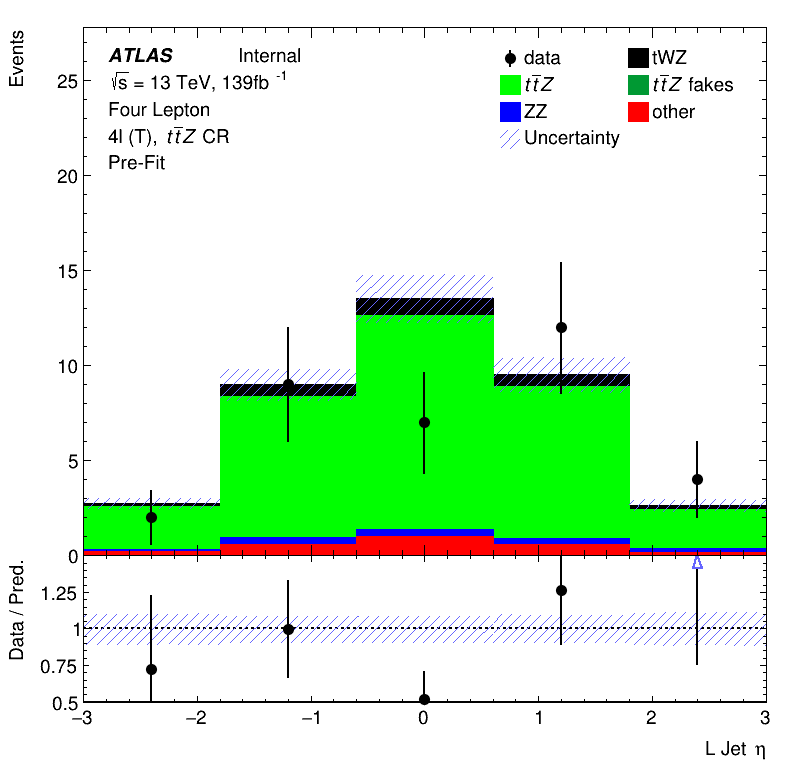
\includegraphics[width=.25\textwidth]{figures/PreFitPlots/lep4_ttZ_4T_LJet_eta.png} &
    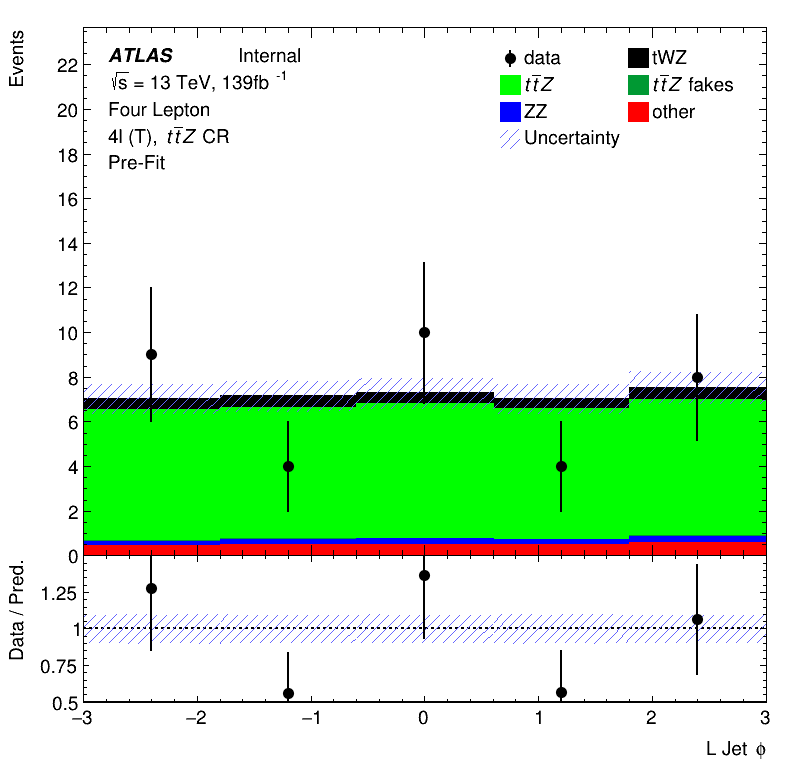
\includegraphics[width=.25\textwidth]{figures/PreFitPlots/lep4_ttZ_4T_LJet_phi.png} \\

  \end{tabular}
    \caption{Comparisons of simulation and data of $p_{T}$, $\eta$ and $\phi$ for leading (L) leptons (top row) and leading (NL) jets (bottom row) in the $t\bar{t}Z$ CR are shown.}\label{fig:4lep-ttZ-CR-leptonPlots}
\end{figure}The majority of the deviations in data and simulation for each plot in Figure \ref{fig:4lep-ttZ-CR-leptonPlots} are within the expected uncertainties. The few plots which have bins where there is a disagreement between data and simulation are either within 2$\sigma$ (L Jet $\phi$) or 3$\sigma$ (L Jet $\eta$) standard uncertainties from one another, or are show more than a 3$\sigma$ (L Lepton $p_{T}$) disagreement. The disagreement in the L Lepton $p_{T}$ distribution could be due to statistical fluctuations in data or simulation, since there are so few events in these bins. In Figure \ref{fig:4lep-ttZ-CR-jets-bjet}, comparisons of simulation and data of $H_{T}$ (scalar sum of Jet $p_{T}$), the Number of jets, the scalar sum of $b$-tagged jet $p_{T}$ and the number of $b$-tagged jets in the $t\bar{t}Z$ CR are shown.
\begin{figure}[htbp]
\centering

    %%%%%%%%%%%%%%%%%
    %%%%% jets %%%%%
    %%%%%%%%%%%%%%%%%

    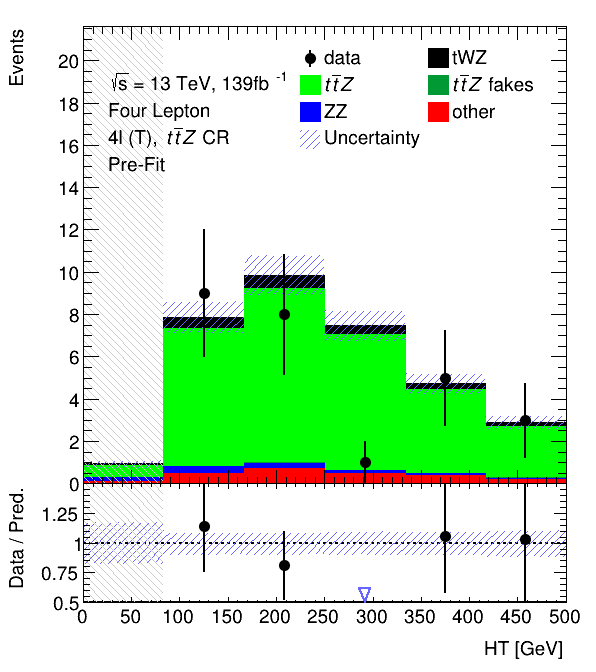
\includegraphics[width=.25\textwidth]{figures/PreFitPlots/lep4_ttZ_4T_HT.png}   \quad
    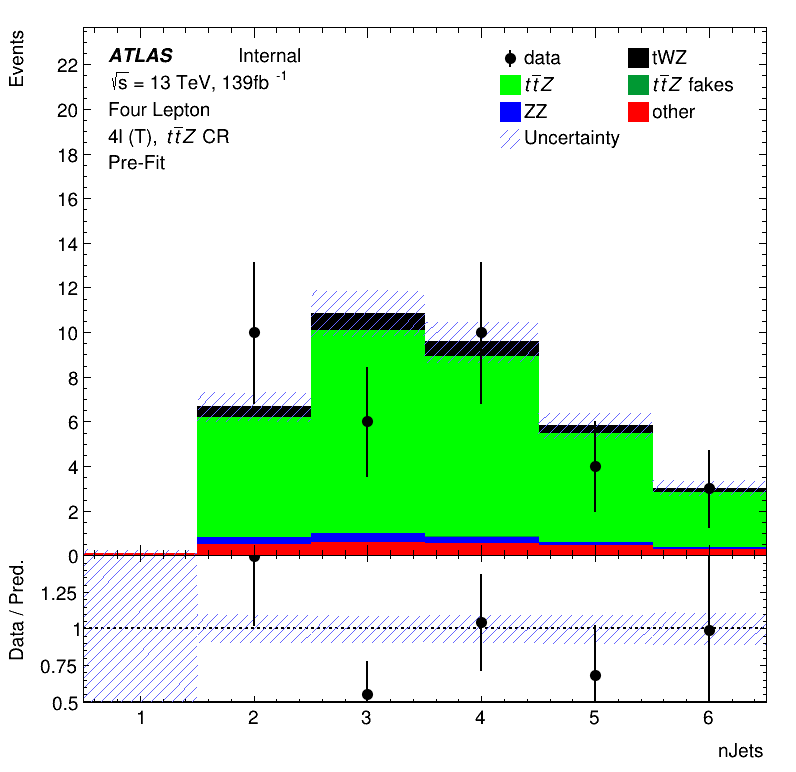
\includegraphics[width=.25\textwidth]{figures/PreFitPlots/lep4_ttZ_4T_Num_Jets.png}
	
	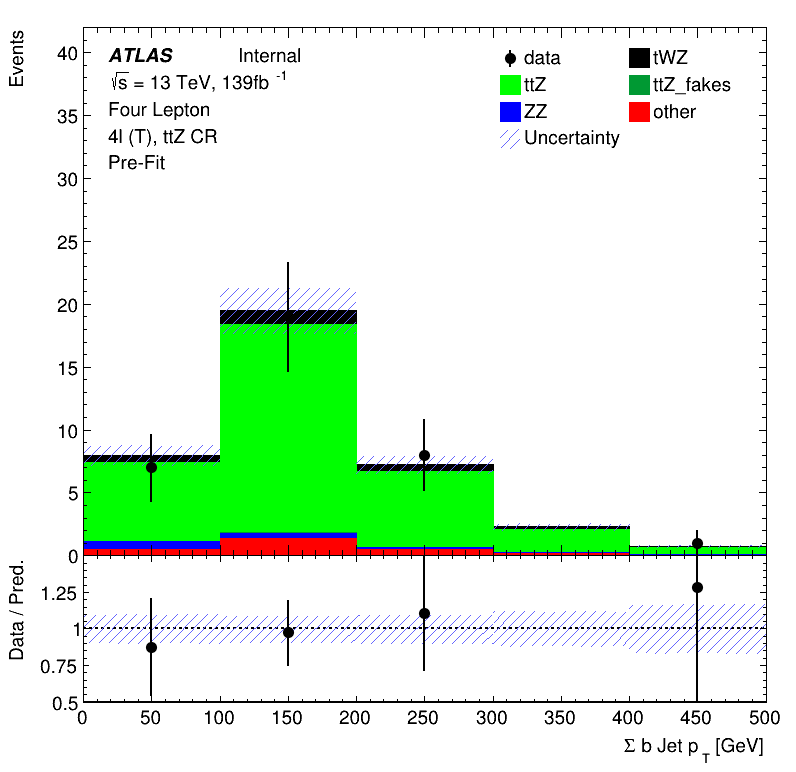
\includegraphics[width=.25\textwidth]{figures/PreFitPlots/lep4_ttZ_4T_sum_bJet_Pt.png}  \quad
    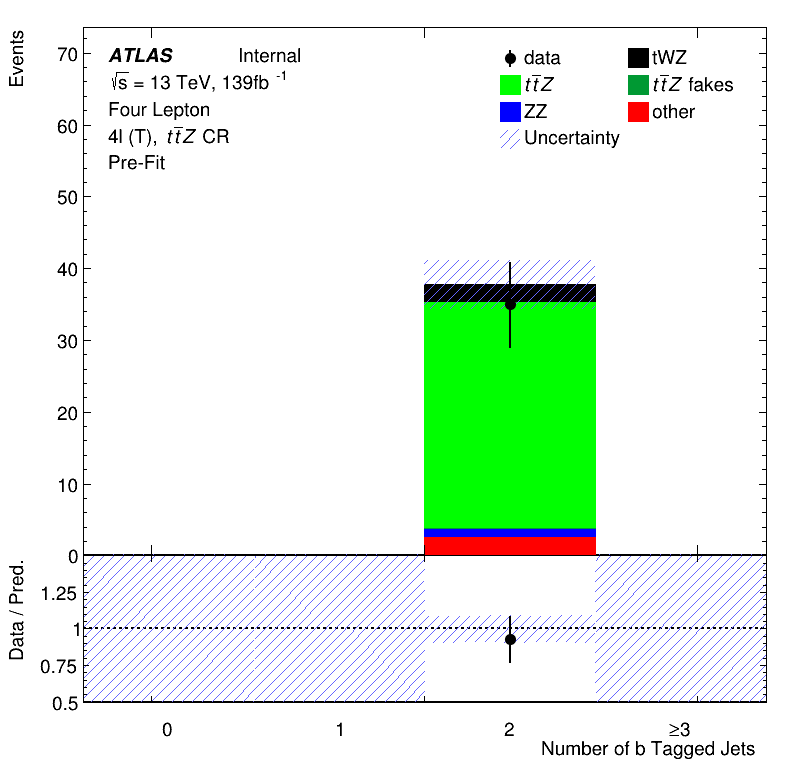
\includegraphics[width=.25\textwidth]{figures/PreFitPlots/lep4_ttZ_4T_Num_bJets.png}

\caption{Comparisons of simulation and data of $H_{T}$ (scalar sum of Jet $p_{T}$), the Number of jets, the scalar sum of $b$-tagged jet $p_{T}$ and the number of $b$-tagged jets (top left to bottom right) in the $t\bar{t}Z$ CR are shown.}\label{fig:4lep-ttZ-CR-jets-bjet} 
\end{figure}Almost all of the deviations in data and simulation for each plot in Figure \ref{fig:4lep-ttZ-CR-jets-bjet} are within the expected uncertainties. There is a 2$\sigma$ disagreement in one of the bins in the nJets distribution and a large disagreement ($> 5\sigma$) in one of the bins in the HT distribution. The large disagreement between data and simulation in the HT distribution is surprising since all other bins in the distribution agree within 1$\sigma$ uncertainties, and it is therefore not fully understood.   


\subsection{$ZZb$ CR}
\label{sec:controlplotstetralepton-ZZb-CR}

%%%%%%%%%%%%%%%%%%%%%%%%%%%%%%%%%%%%
%%%%%%%%%%%%%%%%%%%%%%%%%%%%%%%%%%%%
%%%%%%%      ZZb CR   %%%%%%%%%%
%%%%%%%%%%%%%%%%%%%%%%%%%%%%%%%%%%%%
%%%%%%%%%%%%%%%%%%%%%%%%%%%%%%%%%%%%

In this section, expected number of events of variables in the $ZZb$ CR are shown. In Figure \ref{fig:4lep-ZZb-CR-leptonPlots}, comparisons of simulation and data of $p_{T}$, $\eta$ and $\phi$ for leading (L) leptons and leading (NL) jets in the $ZZb$ CR are shown.
\begin{figure}[htbp]
\centering
  \begin{tabular}{ccc}

    %%%%%%%%%%%%%%%
    %%% Leptons %%%
    %%%%%%%%%%%%%%%

    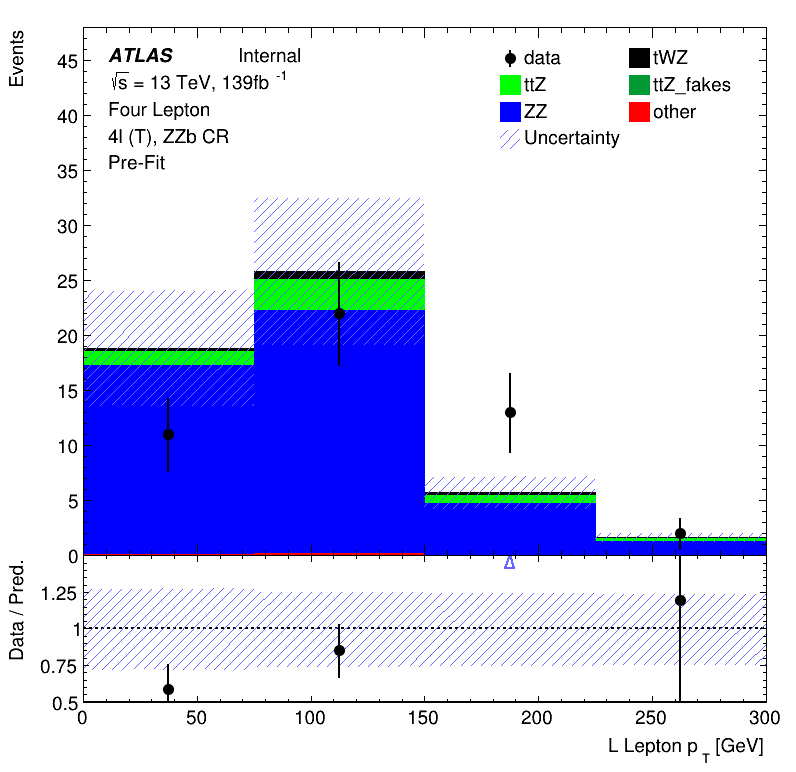
\includegraphics[width=.25\textwidth]{figures/PreFitPlots/lep4_ZZb_4T_L_lepton_pt.png} &
    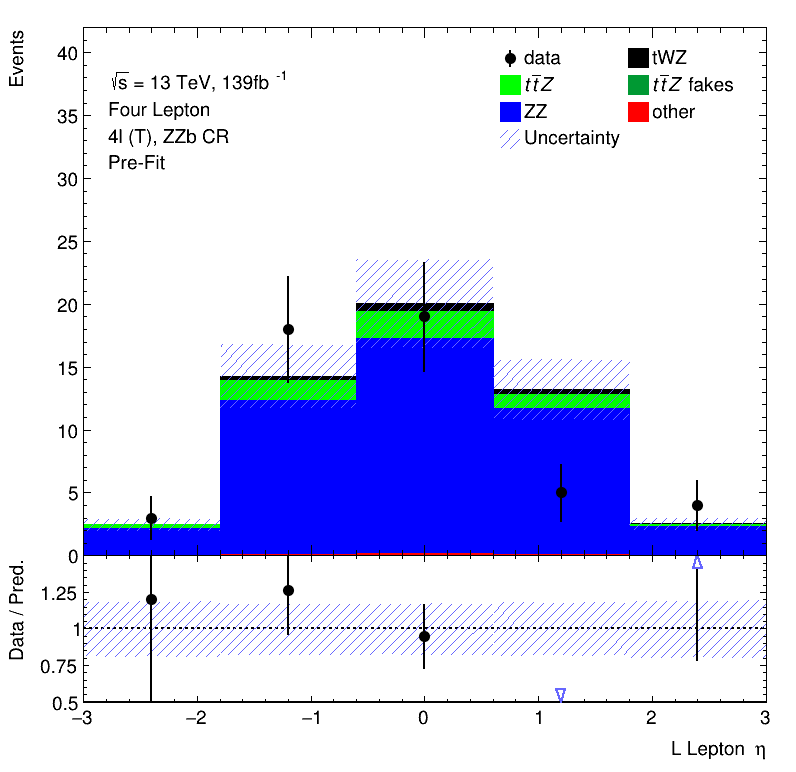
\includegraphics[width=.25\textwidth]{figures/PreFitPlots/lep4_ZZb_4T_L_lepton_eta.png} &
    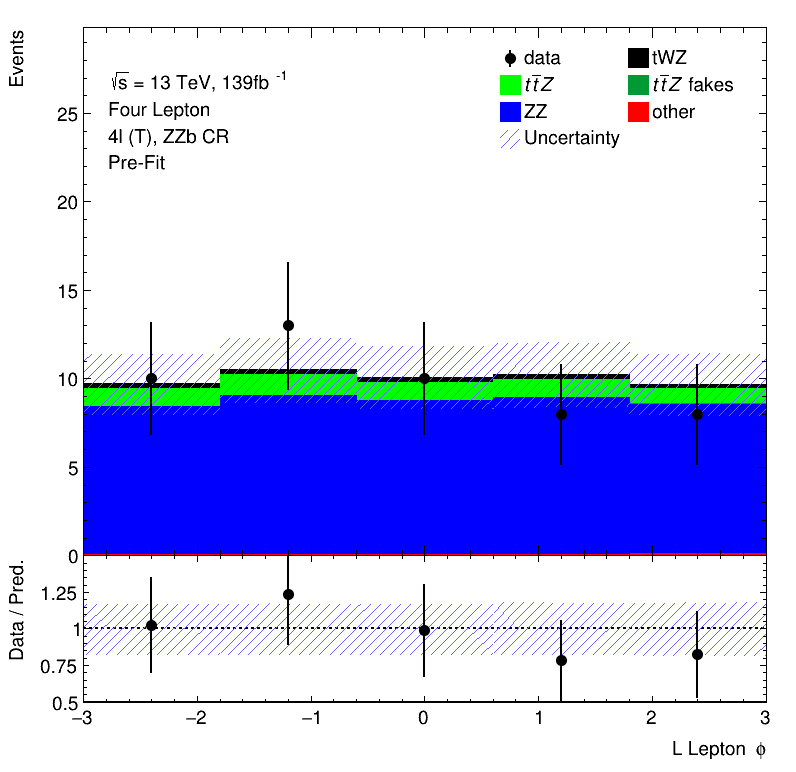
\includegraphics[width=.25\textwidth]{figures/PreFitPlots/lep4_ZZb_4T_L_lepton_phi.png} \\
    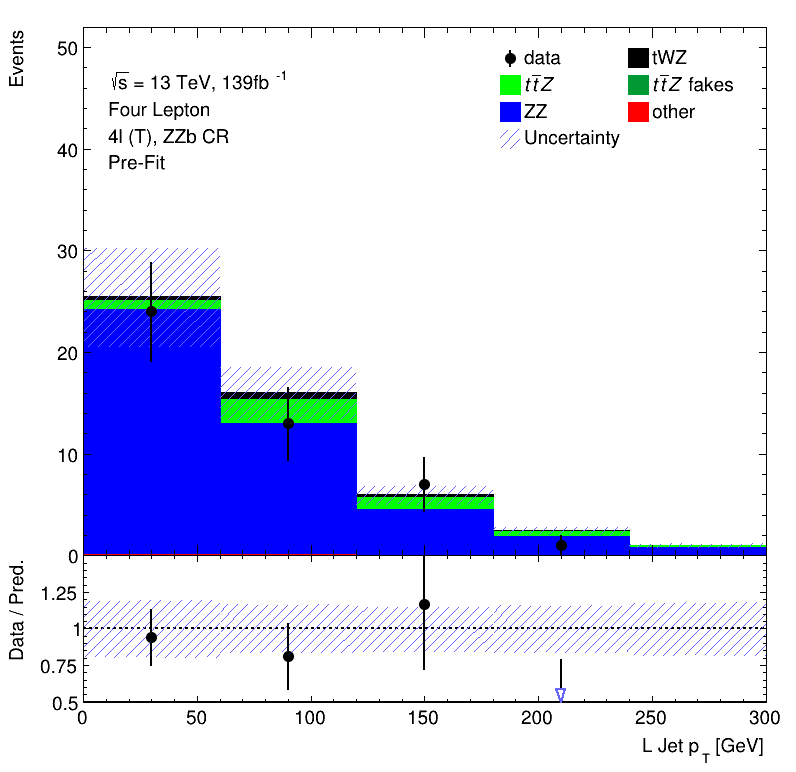
\includegraphics[width=.25\textwidth]{figures/PreFitPlots/lep4_ZZb_4T_LJet_pt.png} &
    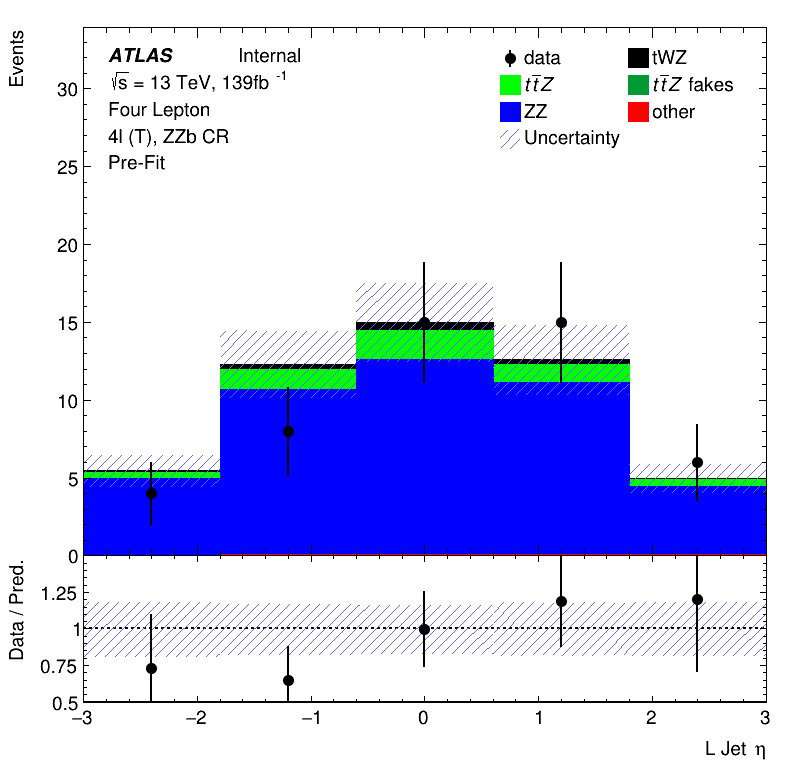
\includegraphics[width=.25\textwidth]{figures/PreFitPlots/lep4_ZZb_4T_LJet_eta.png} &
    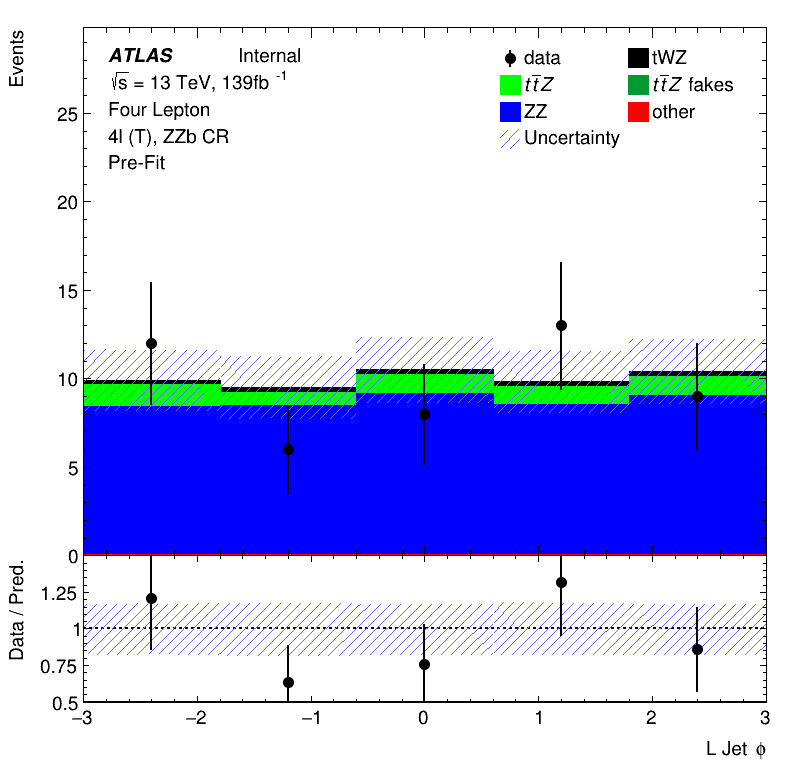
\includegraphics[width=.25\textwidth]{figures/PreFitPlots/lep4_ZZb_4T_LJet_phi.png} \\

  \end{tabular}
    \caption{Comparisons of simulation and data of $p_{T}$, $\eta$ and $\phi$ for leading (L) leptons (top row) and leading (NL) jets (bottom row) in the $ZZb$ CR are shown.}
  \label{fig:4lep-ZZb-CR-leptonPlots}
\end{figure}Most of the deviations in data and simulation for each plot in Figure \ref{fig:4lep-ZZb-CR-leptonPlots} are within the expected uncertainties. There are a few bins with 2$\sigma$ and $> 2\sigma$ disagreements between data and simulation in the L Lepton $p_{T}$, L Lepton $\eta$ and L Jet $p_{T}$ distributions, with the disagreement being much more noticeable in the L Lepton distributions. This could suggest some mis-modelling for L Leptons in this region. In Figure \ref{fig:4lep-ZZb-CR-jets-bjet}, comparisons of simulation and data of $H_{T}$ (scalar sum of Jet $p_{T}$), the Number of jets, the scalar sum of $b$-tagged jet $p_{T}$ and the number of $b$-tagged jets in the $ZZb$ CR are shown.
\begin{figure}[htbp]
 \centering

    %%%%%%%%%%%%%%%%%
    %%%%% jets %%%%%
    %%%%%%%%%%%%%%%%%

    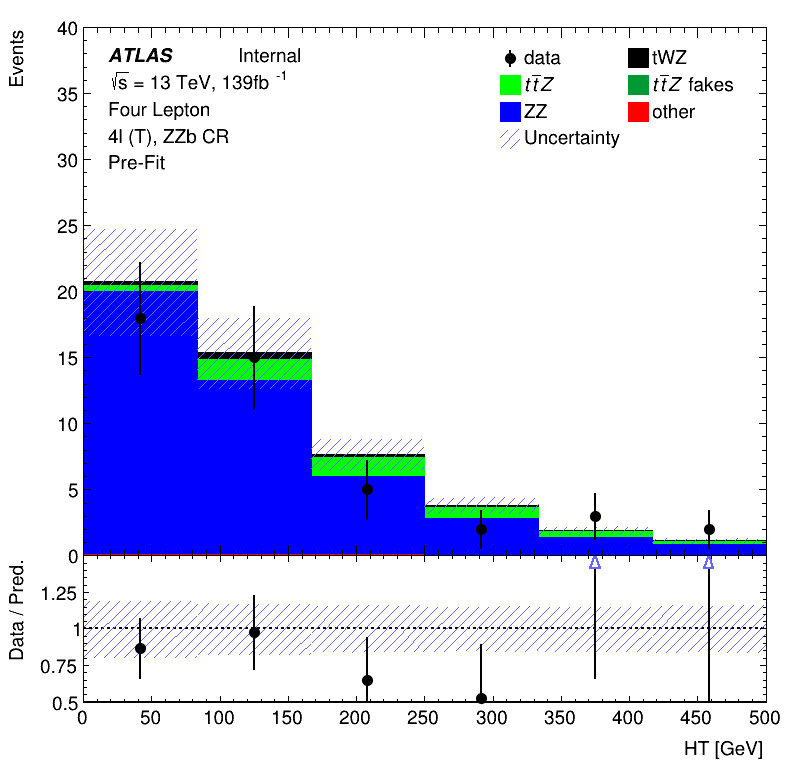
\includegraphics[width=.25\textwidth]{figures/PreFitPlots/lep4_ZZb_4T_HT.png}   \quad
    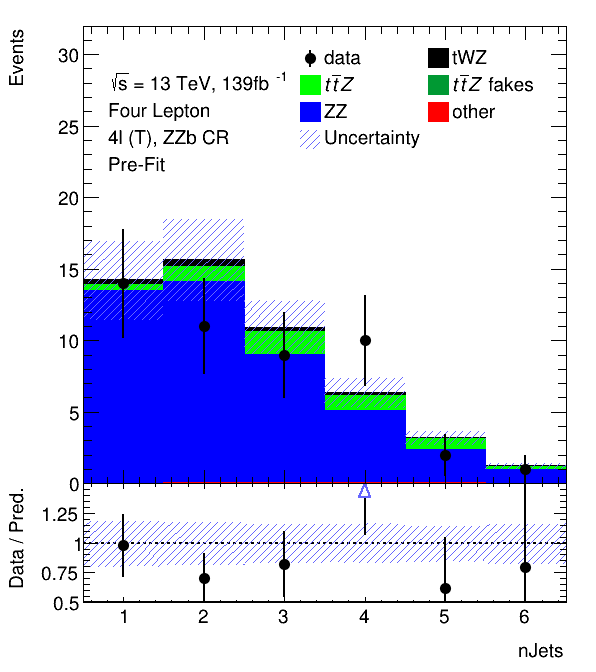
\includegraphics[width=.25\textwidth]{figures/PreFitPlots/lep4_ZZb_4T_Num_Jets.png}
	
	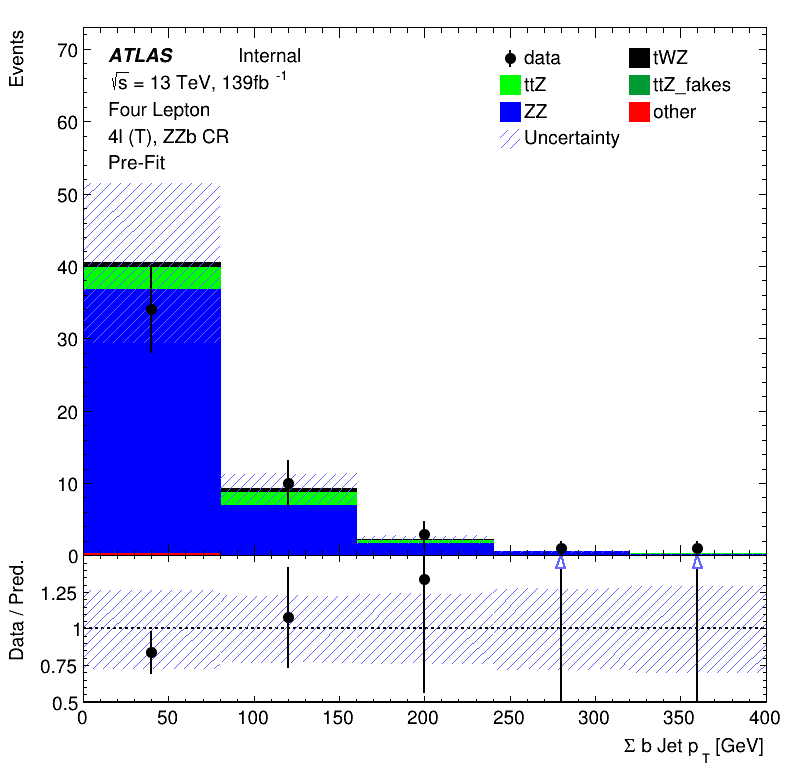
\includegraphics[width=.25\textwidth]{figures/PreFitPlots/lep4_ZZb_4T_sum_bJet_Pt.png}  \quad
    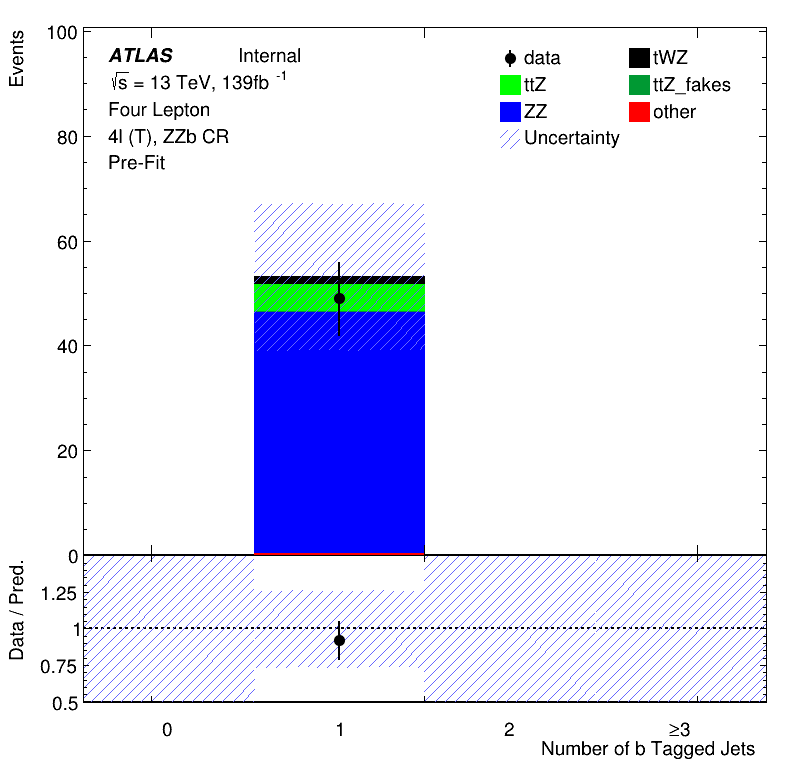
\includegraphics[width=.25\textwidth]{figures/PreFitPlots/lep4_ZZb_4T_Num_bJets.png}

\caption{Comparisons of simulation and data of $H_{T}$ (scalar sum of Jet $p_{T}$), the Number of jets, the scalar sum of $b$-tagged jet $p_{T}$ and the number of $b$-tagged jets (top left to bottom right) in the $ZZb$ CR are shown.}
\label{fig:4lep-ZZb-CR-jets-bjet} 
\end{figure}Most of the deviations in data and simulation for each plot in Figure \ref{fig:4lep-ZZb-CR-leptonPlots} are within the expected uncertainties.


\subsection{$(tWZ)_{\text{fake}}$ CR}
\label{sec:controlplotstetralepton-tWZ-fake-CR}

%%%%%%%%%%%%%%%%%%%%%%%%%%%%%%%%%%%%
%%%%%%%%%%%%%%%%%%%%%%%%%%%%%%%%%%%%
%%%%%%%      tWZ fake CR   %%%%%%%%%%
%%%%%%%%%%%%%%%%%%%%%%%%%%%%%%%%%%%%
%%%%%%%%%%%%%%%%%%%%%%%%%%%%%%%%%%%%

In this section, expected number of events of variables in the \tWZfake CR are shown. In Figure \ref{fig:4lep-tWZ-fake-CR-leptonPlots}, comparisons of simulation and data of $p_{T}$, $\eta$ and $\phi$ for leading (L) leptons and leading (NL) jets in the \tWZfake CR are shown.
\begin{figure}[htbp]
\centering
  \begin{tabular}{ccc}

    %%%%%%%%%%%%%%%
    %%% Leptons %%%
    %%%%%%%%%%%%%%%

    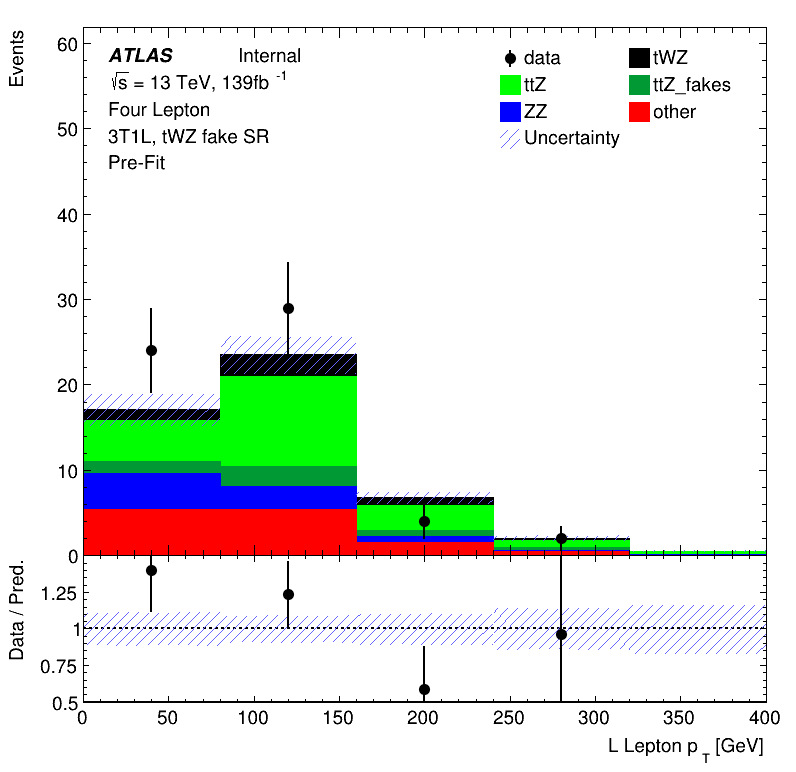
\includegraphics[width=.25\textwidth]{figures/PreFitPlots/lep4_tWZ_3T1L_L_lepton_pt.png} &
    \includegraphics[width=.25\textwidth]{figures/PreFitPlots/lep4_tWZ_3T1L_L_lepton_eta.png} &
    \includegraphics[width=.25\textwidth]{figures/PreFitPlots/lep4_tWZ_3T1L_L_lepton_phi.png} \\
    \includegraphics[width=.25\textwidth]{figures/PreFitPlots/lep4_tWZ_3T1L_LJet_pt.png} &
    \includegraphics[width=.25\textwidth]{figures/PreFitPlots/lep4_tWZ_3T1L_LJet_eta.png} &
    \includegraphics[width=.25\textwidth]{figures/PreFitPlots/lep4_tWZ_3T1L_LJet_phi.png} \\

\end{tabular}
\caption{Comparisons of simulation and data of $p_{T}$, $\eta$ and $\phi$ for leading (L) leptons (top row) and leading (NL) jets (bottom row) in the \tWZfake CR are shown.}
\label{fig:4lep-tWZ-fake-CR-leptonPlots}
\end{figure}The vast majority of bins in each plot in Figure \ref{fig:4lep-tWZ-fake-CR-leptonPlots} have $\frac{signal}{background}$ exceeding 0.1 and are therefore blinded. This region is therefore enriched in $tWZ$ signal events. Most deviations in data and simulation in the bins which are not blinded, are within the expected uncertainties. Only two out of seven unblinded bins are not within expected uncertainties and are within a 2$\sigma$ uncertainty. In Figure \ref{fig:4lep-tWZ-fake-CR-jets-bjet}, comparisons of simulation and data of $H_{T}$ (scalar sum of Jet $p_{T}$), the Number of jets, the scalar sum of $b$-tagged jet $p_{T}$ and the number of $b$-tagged jets in the \tWZfake CR are shown.
\begin{figure}[htbp]
 \centering

    %%%%%%%%%%%%%%%%%
    %%%%% jets %%%%%
    %%%%%%%%%%%%%%%%%

    \includegraphics[width=.25\textwidth]{figures/PreFitPlots/lep4_tWZ_3T1L_HT.png}   \quad
    \includegraphics[width=.25\textwidth]{figures/PreFitPlots/lep4_tWZ_3T1L_Num_Jets.png}
	
	\includegraphics[width=.25\textwidth]{figures/PreFitPlots/lep4_tWZ_3T1L_sum_bJet_Pt.png}  \quad
    \includegraphics[width=.25\textwidth]{figures/PreFitPlots/lep4_tWZ_3T1L_Num_bJets.png}

\caption{Comparisons of simulation and data of $H_{T}$ (scalar sum of Jet $p_{T}$), the Number of jets, the scalar sum of $b$-tagged jet $p_{T}$ and the number of $b$-tagged jets (top left to bottom right) in the \tWZfake CR are shown.}
\label{fig:4lep-tWZ-fake-CR-jets-bjet} 
\end{figure}The majority of bins in each plot in Figure \ref{fig:4lep-tWZ-fake-CR-jets-bjet} have $\frac{signal}{background}$ exceeding 0.1 and are therefore blinded. This region is therefore enriched in $tWZ$ signal events. Most deviations in data and simulation in the bins which are not blinded, are within the expected uncertainties. Only two out of seven unblinded bins are not within expected uncertainties and are within a 2$\sigma$ uncertainty.

\section{Fake Lepton Estimation}
\label{sec:fakelepest}
Fake leptons are physics objects reconstructed as leptons, but do not correspond to the leptons which originate from the hard scatter process or those physics objects that are mis-identified as leptons. The sources of fake leptons include those originating from heavy hadron decays, light hadron decays or via the conversion of a photon to a lepton. In the ATLAS detector, the probability for a fake to occur is very low. In this section, the method used to estimate the fake lepton contribution is described.\\

As \ttZ is the dominant background process ($\sim$ 75$\%$ of the total background contribution), it is assumed that \ttZ will also dominate the events containing fake leptons. The fake lepton efficiency, $\epsilon$, can be written as $\epsilon = \frac{N_{\text{fake}}^{\text{tight}}}{N_{\text{fake}}^{\text{loose}}}$, where $N_{\text{fake}}^{\text{tight}}$ is the number of fake leptons which pass the tight lepton selection (See Section \ref{sec:lepton-object}) and $N_{\text{fake}}^{\text{loose}}$ is the number of fake leptons which pass the loose lepton selection (See Section \ref{sec:lepton-object}). The probability of one fake lepton to occur, $P(\text{one fake }\ell)$, is proportional to $\epsilon_{1} \ll 1$~\cite{lesage2017lepton, ATLAS-CONF-2012-048} and the probability for two fakes to occur is, $P(\text{two fakes }\ell)$, is proportional to $\epsilon_{2} < \epsilon_{1} \ll 1$. In this analysis, an estimation of the fake lepton component to the highest order is investigated and therefore the case where at least one fake lepton occurs in a \ttZ event is considered.\\

Firstly, the dominant \ttZ background is split up into \ttZ and $(t\bar{t}Z)_{\text{fake}}$ components. Secondly, a $(tWZ)_{\text{fake}}$ CR (See Section \ref{sec:regionsAndEventSelection}) is defined which is enhanced in fakes and aims to constrain the $(t\bar{t}Z)_{\text{fake}}$ background in the SR. All events which contribute to the $(t\bar{t}Z)_{\text{fake}}$ background are determined by the \texttt{IFF Truth Classifier}~\cite{IFFTruthClassifier}. The \texttt{IFF Truth Classifier} is a tool which aims to classify leptons based off their truth information. It uses the more general \texttt{MCTruthClassifier}~\cite{MCTruthClassifier} tool's output as input and returns one of the following lepton categories: \texttt{Unknown}, \texttt{KnownUnknown} (leptons which can (in priciple) be classified, but the \texttt{MCTruthClassifier} fails to classify the lepton's truth type or origin), \texttt{IsoElectron}, \texttt{ChargeFlipIsoElectron}, \texttt{PromptMuon}, \texttt{PromptPhotonConversion}, \texttt{ElectronFromMuon}, \texttt{TauDecay}, \texttt{BHadronDecay}, \texttt{CHadronDecay} or \texttt{LightFlavorDecay} (More details~\cite{IFFTruthClassifier}). Given these categories, leptons are considered as fake if they are classified as \texttt{PromptPhotonConversion}, \texttt{BHadronDecay}, \texttt{CHadronDecay} or \texttt{LightFlavorDecay} (i.e. a lepton originating from the decay of a $b$-Hadron, $c$-Hadron or light-flavour jet). Events which contribute to the $(t\bar{t}Z)_{\text{fake}}$ background are those where at least one lepton from the \ttZ sample are classified by the \texttt{IFF Truth Classifier} with one of the four aforementioned categories.\\

The $(tWZ)_{\text{fake}}$ CR aims to be as similar as possible to the $tWZ$ SRs, but enhanced in fakes. This CR can then be used to constrain the normalisation of the $(t\bar{t}Z)_{\text{fake}}$ template. To ensure that this region is enhanced in fakes, it is required that it contains 3 tight leptons and 1 loose lepton, since loose leptons are more likely to be fakes. Leptons from heavy decays are produced in jets and are typically surrounded by other energetic particles. Since the loose lepton definition relaxes the isolation requirement, leptons satisfying the loose criteria are more enhanced in these fake leptons. By using the $p_{T}$ of the loose lepton ($p_{T}(\text{Loose Lepton})$) in this region as the variable used in the fit, the shape (and normalisation) of the $(t\bar{t}Z)_{\text{fake}}$ template can be constrained. In Figure \ref{fig:4lep-iff-bar1}, the number of leptons classified as fake and the relative dominance of the different classifications for fake leptons, split up by their IFF Truth classification, in each region are shown.

\begin{figure}[htbp]
\centering

    \includegraphics[width=.47\textwidth]{figures/iff_bar_1.png}   
     \includegraphics[width=.47\textwidth]{figures/iff_bar_2.png} 

    \caption{\textbf{Left: }The number of leptons classified as fake, split up by their IFF Truth classification, in each region is shown. The left panel shows the number of leptons classified as fakes, scaled by a factor of 50, on the y-axis. The right panel shows the number of leptons classified as fakes (unscaled), on the y-axis. The different signal and control regions are shown on the x-axes of the left and right panels. The different coloured stacked histograms correspond to the IFF truth classification of the leptons, as shown in the legend. \textbf{Right: }The relative dominance of the different classifications for fake leptons (classified by the IFF truth classified) in each region, is shown. The relative dominance of leptons classified as fakes, as a fraction of the total number of fake leptons (in each region), is shown on the y-axis. The different signal and control regions are shown on the x-axis. The different coloured stacked histograms correspond to the IFF truth classification of the leptons, as shown in the legend.}
  \label{fig:4lep-iff-bar1}
\end{figure}The plot on the left illustrates that there is a large amount of fake leptons which pass our selection criteria for the $(tWZ)_{\text{fake}}$ CR, compared to remaining four regions. Therefore there is a significant amount of fake leptons present in the $(tWZ)_{\text{fake}}$ CR which allow the fake lepton component to be sufficiently constrained. The plot on the right illustrates that the majority of fake leptons which pass our selection criteria originate from the decay of $b$-hadrons, in all regions but the $t\bar{t}Z$ CR. The smaller proportion of fake leptons originating from $b$-hadron decays in the $t\bar{t}Z$ CR could possibly be due to statistical fluctuations resulting from the low number of fake leptons which pass our selection criteria in this region ($\sim 40$ fake leptons). In Figure \ref{fig:4lep-iff-bar3}, the amount of fake and real $t\bar{t}Z$ events which pass our selection criteria, in each region, is shown.
\begin{figure}[htbp]
\centering

    \includegraphics[width=.65\textwidth]{figures/iff_bar_3.png}   

    \caption{The percentage of fake and real $t\bar{t}Z$ events which pass our selection criteria, in each region, is shown. The relative number of fake and real events (in $\%$ of the total number of events in the nominal and fake $t\bar{t}Z$ background samples) is shown on the y-axis. The different signal and control regions are shown on the x-axis. The blue and red histograms represent the percentage of real and fake events (out of the total number of events in the nominal and fake $t\bar{t}Z$ background samples), respectively. }
  \label{fig:4lep-iff-bar3}
\end{figure}Around 20$\%$ of all $t\bar{t}Z$ events are classified as fake events (having one or more of its leptons being classified as fake) in the $(tWZ)_{\text{fake}}$ CR. The $tWZ$ OF SR, $tWZ$ SF SR, $t\bar{t}Z$ CR and $ZZb$ CR have less than 1$\%$ of their total $t\bar{t}Z$ events being fake. The significant fraction of fake $t\bar{t}Z$ events present in the $(tWZ)_{\text{fake}}$ CR allows the $t\bar{t}Z$ fake background to be sufficiently constrained by the $(tWZ)_{\text{fake}}$ CR.


\section{Improving signal vs background discrimination}
The presence of different numbers of top quarks is a key discriminator between signal and the dominant background process, $t\bar{t}Z$. This information is aimed to be exploited by reconstructing $\ell b$ systems as a proxy for top quarks (since, $t\rightarrow W(\rightarrow \ell \nu) b$). This is done in two ways, firstly, by implementation of a kinematic reconstruction algorithm (Two Neutrino Scanning Method) which aims to determine the likelihood of an event containing two top quarks and secondly, by implementing a Boosted Decision Tree (BDT) which is used to distinguish between $\ell b$ systems that originate from top quarks and $\ell b$ systems which do not originate from top quarks. In this thesis, this BDT is referred to as an \textit{object-level} BDT. Certain variables constructed from event information show discrimination between signal and background events. This information can be exploited to discriminate between signal and background events by constructing a BDT which uses these discriminating variables for training. A BDT is implemented and is used to discriminate between \tWZ events and its major backgrounds, \ttZ and \ZZ. Furthermore, this BDT takes information from the kinematic reconstruction algorithm and the object-level BDT in order to maximize its discriminating power. In this thesis, this BDT is referred to as an \textit{event-level} BDT. The discriminator output from the object-level BDT can be converted to a variable which can then be used as an input to the event-level BDT.
\subsection{Two Neutrino Scanning Method (2$\nu$SM) Algorithm}
\label{sec:2vsm}
The difference in the number of resonant top quarks in the $tWZ$ signal and the dominant background, $t\bar{t}Z$, is a key feature which can be exploited in order to discriminate between these two processes. In Section \ref{sec:object-level-bdt}, a BDT was implemented which exploits this information by aiming to identify $\ell b$ systems originating from top quarks. In this section, a kinematic reconstruction algorithm (Two Neutrino Scanning Method) is implemented which exploits the same feature. The Two Neutrino Scanning Method (2$\nu$SM) algorithm\footnote{software tool and weights provided by Thomas McCarthy (\ttZ analysis group - Max Planck Institute)}~\cite{2vSM-ref1,2vSM-ref2} aims to reconstruct $t\bar{t}$ systems in the 2$\ell$, 3$\ell$ and 4$\ell$ final states (e.g. 2$\ell$ case: $t\bar{t}\rightarrow \ell^{+}\nu_{\ell}b\ell^{-}\bar{\nu}_{\ell}\bar{b}$). The 2$\nu$SM algorithm aims to reconstruct a $t\bar{t}$ system by finding two neutrinos ($\nu_{1}$ and $\nu_{2}$) which are most likely to correspond to the neutrinos that originate from the decay of a $t\bar{t}$ system. This algorithm can be used in our analysis to discriminate between \tWZ and \ttZ, since the OSSF leptons which decay from the $Z$ boson can be easily reconstructed and removed before inputting the event into the algorithm. The removal of the $Z$ boson results in \tWZ events that don't resemble $t\bar{t}$ systems and \ttZ events that do resemble $t\bar{t}$ systems, which the algorithm is designed to distinguish between. It would then be expected that the 2$\nu$SM algorithm returns a higher score from a \ttZ event ($\sim$ 1, i.e. it resembles a $t\bar{t}$ event after removal of the $Z$ boson) and a lower score from a \tWZ event ($\sim$ 0, i.e. it does not resemble a $t\bar{t}$ event after removal of the $Z$ boson). The first step in the $2\nu$SM algorithm involves stating four equations which correspond to the invariant masses of the top quark ($m(t)$) and $W$ boson ($m(W)$) for the two top quark decays (i.e. $t\rightarrow W^{+}b \rightarrow \ell^{+} \nu_{\ell}$) in a dileptonic $t\bar{t}$ event. These can be written as,

\begin{align}
    (\ell_{1} + \nu_{1})^{2} &= m(W)^{2} = (\SI{80.385}{GeV})^2\\
    (\ell_{1} + \nu_{1} + b_{1,2})^{2} &= m(t)^{2} = (\SI{172.5}{GeV})^{2}\\
    (\ell_{2} + \nu_{2})^{2} &= m(W)^{2} = (\SI{80.385}{GeV})^2\\
       (\ell_{2} + \nu_{2} + b_{2,1})^{2} &= m(t)^{2} = (\SI{172.5}{GeV})^{2}
\end{align}where the subscripts indicate that these particles originate from the decay of two different top quarks in a $t\bar{t}$ system. An assumption is made such that the mass of the neutrinos ($\nu_{1}$ and $nu_{2}$) are exactly zero, which leaves us with 6 unknowns, $p_{{T}_{\nu_{1}}}$, $\phi_{\nu_{1}}$, $\eta_{\nu_{1}}$, $p_{{T}_{\nu_{2}}}$, $\phi_{\nu_{2}}$ and $\eta_{\nu_{2}}$ (components of the two neutrino's 4-vectors). The 4-vectors of the two reconstructed leptons (not from the $Z$ boson) and the two jets with the highest DL1r $b$-tagger score are used as input to the algorithm. For each neutrino ($\nu_{1}$ and $\nu_{2}$), a scan over a range of possible $\eta$ and $\phi$ values is performed. These values were chosen to be $\phi_{\nu_{1}}$, $\phi_{\nu_{2}} \in [-\pi,\pi]$ with a step size of $\approx$ 0.25 and $\eta_{\nu_{1}}$, $\eta_{\nu_{2}} \in [-5,5]$ with a step size of $\approx$ 0.31. These ranges were chosen to maximize accuracy and minimize computation time. For each of these possible $\eta$ and $\phi$ values, the corresponding $p_{T}$ for each neutrino is calculated ($p_{{T}_{\nu_{1}}}$ and $p_{{T}_{\nu_{2}}}$) via,

\begin{equation}
    p_{{T}_{\nu}} = \frac{\frac{1}{2} (m(W)^{2} - m(\ell)^{2})}{E_{\ell}\cosh{\eta_{\nu}} - p_{\ell,z}\sinh{\eta_{\nu}} - p_{\ell,x}\cos{\phi_{\nu}} - p_{\ell,y}\sin{\phi_{\nu}} }
\end{equation}where $E_{\ell}$ is the energy of the lepton, $m(\ell)$ is the invariant mass of the lepton and $p_{\ell, z}$, $p_{\ell, x}$, $p_{\ell, y}$ are the $z$, $x$ and $y$ components of lepton's momentum. After computing $p_{{T}_{\nu}}$ for both neutrinos for each possible $\eta$ and $\phi$ combination in the defined ranges, a collection of possible 4-vectors for $\nu_{1}$ and $\nu_{2}$ can be reconstructed. Using $\nu_{1}$ and $\nu_{2}$, two possible $t\bar{t}$ systems are reconstructed,
\begin{align}
    t_{1} = \ell_{1} + b_{1} + \nu_{1} &\text{ and } t_{2} = \ell_{2} + b_{2} + \nu_{2} \label{eq:top1-2vSM}\\
    &\textbf{OR}\nonumber\\ 
     t_{1} = \ell_{1} + b_{2} + \nu_{1} &\text{ and } t_{2} = \ell_{2} + b_{1} + \nu_{2} \label{eq:top2-2vSM}
\end{align}The 2$\nu$SM algorithm is extremely computationally intensive. The computation time depends on the number step size of the $\phi$ and $\eta$ ranges which are scanned over to reconstruct the neutrinos. For example, consider the step sizes chosen in this analysis, $\Delta \eta \approx$ 0.31 and $\Delta \phi \approx$ 0.25 which corresponds to 32 values for $\eta$ and 25 values for $\phi$. There will be $(32)(32)(25)(25) = $ 640 000 possible pairs of neutrinos ($\nu_{1}$ and $\nu_{2}$) to consider per event. Since two possible $t\bar{t}$ systems (See Equations \ref{eq:top1-2vSM} and \ref{eq:top2-2vSM}) are considered, this number effectively increases to $(2)(640000) = $ 128 000 0 iterations per event. In order to reduce the number of $t\bar{t}$ systems needed to be considered, therefore decreasing computation time, distributions of variables from $t\bar{t}$ events are studied to apply a veto to a possible reconstructed $t\bar{t}$ system if the variable in question is improbable or unlikely to be observed in a $t\bar{t}$ event. To achieve this, an allowed range is defined for these variables (See Figure \ref{fig:eta-bbll-heatmap} and Figure \ref{fig:lt-heatmap}), and if the possible reconstructed $t\bar{t}$ system's corresponding value for this variable lies outside this range, it is vetoed and the algorithm continues with the next iteration. The first variable which is considered, is the difference between average mass of the two possible $\ell b$ system combinations, $\Delta \langle m(\ell b)\rangle$. The two possible $\ell b$ system combinations are,

\begin{align}
    (\ell_{1} b_{1}) = \ell_{1} + b_{1} &\text{ and }  (\ell_{2} b_{2})  = \ell_{2} + b_{2} \\
    &\textbf{OR}\nonumber\\ 
     (\ell_{1} b_{2}) = \ell_{1} + b_{2} &\text{ and }  (\ell_{2} b_{1})  = \ell_{2} + b_{1} 
\end{align}$\Delta \langle m(\ell b) \rangle$ is therefore defined as,

\begin{equation}
    \Delta \langle m(\ell b) \rangle = \frac{1}{2} \abs{[( m(\ell_{1} b_{1}) + m(\ell_{2} b_{2}) ) - ( m(\ell_{1} b_{2}) + m(\ell_{2} b_{1}) ]}
\end{equation}The idea here is that, in events where the average masses of the two possible $\ell b$ system combinations differ greatly, the correct combination is likely to be given by the combination with the smaller average mass. Furthermore, it was shown in Ref.~\cite{2vSM-ref1} that reconstructed top quarks in a $t\bar{t}$ system that contain $b$-tagged jets in opposite hemispheres\footnote{The ATLAS detector can be split into two regions or \textit{hemispheres}, defined where $z > 0$ and $z < 0$} ($\eta(b_{1}) \times \eta(b_{2}) < 0$) of the ATLAS detector are easier to determine the correct $\ell b$ system combination than reconstructed $t\bar{t}$ systems that contain $b$-tagged jets in the same hemispheres ($\eta(b_{1}) \times \eta(b_{2}$). To illustrate this, the distributions (constructed from $t\bar{t}$ events) of the probability of choosing the correct $\ell b$ system combination, given that the one with the minimum $\langle m(\ell b) \rangle)$ chosen ($P(\text{Correct combination of } \ell b \text{ systems} | \text{minimum} \langle m(\ell b) \rangle)$) vs $\Delta \langle m(\ell b) \rangle$ for $b$-tagged jets in the same and opposite hemispheres are investigated. In Figure \ref{fig:lb-assoc}, the $P(\text{Correct combination of } \ell b \text{ systems} | \text{minimum} \langle m(\ell b) \rangle)$ vs $\Delta \langle m(\ell b) \rangle$, for $b$-tagged jets in the same and opposite hemispheres, constructed from $t\bar{t}$ events are shown.
\begin{figure}[h!]
	\includegraphics[width=0.6\linewidth]{figures/lbassoc_2vSM.png}
	\centering
	\caption{$P(\text{Correct combination of } \ell b \text{ systems} | \text{minimum} \langle m(\ell b) \rangle)$ vs $\Delta \langle m(\ell b) \rangle$, for $b$-tagged jets in the same and opposite hemispheres, constructed from $t\bar{t}$ events is shown. The horizontal red lines represent the distribution in the case when the two $b$-jets are in opposite hemispheres. The dot in the middle of the line represents the midpoint of the line. The horizontal black lines represent the distribution in the case when the two $b$-jets are in the same hemispheres. The dot in the middle of the line represents the midpoint of the line. The average $m(\ell b)$ is shown on the x-axis. The $P(\text{Correct combination of } \ell b \text{ systems} | \text{minimum} \langle m(\ell b) \rangle)$ is shown on the y-axis.}
	\label{fig:lb-assoc}
\end{figure}From Figure \ref{fig:lb-assoc}, for both cases where the $b$-tagged jets are in the same and opposite hemispheres, the probability for a correct $\ell b$ system being chosen, given that the $\ell b$ system with the minimum average mass is under consideration, is an increasing function which plateaus to 1 at $\sim$ \SI{90}{\GeV}. One of these two distributions are used (depending on whether or not the two $b$-tagged jets are in the same or opposite hemispheres) to interpolate the $P(\text{Correct combination of } \ell b \text{ systems} | \text{minimum} \langle m(\ell b) \rangle)$ from $\Delta \langle m(\ell b) \rangle$. A veto is applied to the $\ell b$ combination with the maximum $\Delta \langle m(\ell b) \rangle$ if $P(\text{Correct combination of } \ell b \text{ systems} | \text{minimum} \langle m(\ell b) \rangle) > 0.8$, indicating that there is at least an 80$\%$ certainty that the $\ell b$ combination with the minimum $\langle m(\ell b) \rangle$ is the correct combination. If $P(\text{Correct combination of } \ell b \text{ systems} | \text{minimum} \langle m(\ell b) \rangle) < 0.8$, both possible $\ell b$ system combinations need to be considered. The $\eta$ of the $b\bar{b}\ell\ell$ system, $\eta(b\bar{b}\ell\ell)$, to veto improbable $\eta(\nu_{1})$ and $\eta(\nu_{2}$) values is then considered. In the same way as for $\Delta \langle m(\ell b)\rangle$, a distribution is generated to determine values $\eta(\nu)$ which are improbable for a $t\bar{t}$ event. In this case, a 2D histogram from simulated $t\bar{t}$ events (dileptonic final state) at generator-level of $\eta (\nu)$ vs $\eta(b\bar{b}\ell\ell)$ is generated. Using this histogram, a veto region (where a $t\bar{t}$ event is extremely unlikely to occur) is defined which contains 95$\%$ of events. A veto is applied if either possible neutrino lies within this region. In Figure \ref{fig:eta-bbll-heatmap}, a heatmap of occupancy for $\eta (\nu)$ vs $\eta(b\bar{b}\ell\ell)$ (produced from simulated $t\bar{t}$ events)  and its corresponding veto region are shown. 
 \begin{figure}[h!]
	\includegraphics[width=0.45\linewidth]{figures/bbll_occ_2vSM.pdf}
		\includegraphics[width=0.45\linewidth]{figures/bbll_veto_2vSM.pdf}
	\centering
	\caption{\textbf{Left: }Heatmap of occupancy for $\eta (\nu)$ vs $\eta(b\bar{b}\ell\ell)$ produced from simulated $t\bar{t}$ events (dileptonic final state) at generator-level is shown. $\eta$ of the $b\bar{b}\ell\ell$ system is shown on the x-axis. $\eta$ of the neutrino is shown on the y-axis. The colourbar on the right represents the fraction of events in the phase space. \textbf{Right: } The regions where vetoes are applied for the $\eta(b_{1}b_{2}\ell_{1}\ell_{2})$ constraint is shown. $\eta$ of the $b\bar{b}\ell\ell$ system is shown on the x-axis. $\eta$ of the neutrino is shown on the y-axis. The red band shows the region where the neutrino would not be vetoed. The white areas (above and below the red band) are regions where the neutrino is vetoed.}
	\label{fig:eta-bbll-heatmap}
\end{figure}The final kinematic constraint which is considered is the scalar sum of lepton $p_{T}$, $L_{T} = p_{T}(\ell_{1}) + p_{T}(\ell_{2})$, which is used to veto certain possible neutrinos, $\nu_{1}$ and $\nu_{2}$. Again, a distribution is generated to determine (and veto) improbable possible neutrinos in simulated $t\bar{t}$ events (dilepton final state). Using the same method as described for Figure \ref{fig:eta-bbll-heatmap}, a veto region is defined where a veto is applied if either possible neutrino lies within this region. In Figure \ref{fig:lt-heatmap}, a heatmap of occupancy for $\Delta R (\ell, \nu)$ vs $L_{T}$ (produced from simulated $t\bar{t}$ events) and its corresponding veto region are shown.
 \begin{figure}[h!]
	\includegraphics[width=0.45\linewidth]{figures/lt_occ_2vSM.pdf}
	\includegraphics[width=0.45\linewidth]{figures/lt_veto_2vSM.pdf}
	\centering
	\caption{\textbf{Left: }A heatmap of occupancy for $\Delta R (\ell, \nu)$ vs $L_{T}$ produced from simulated $t\bar{t}$ events (dileptonic final state) at generator-level is shown. $\Delta R$ between leptons and neutrinos is shown on the x-axis. $L_{T}$ (scalar sum of lepton $p_{T}$) is shown on the y-axis. The colourbar on the right represents the fraction of events in the phase space. \textbf{Right: }The regions where vetoes are applied for the $L_{T}$ constraint is shown. $\Delta R$ between leptons and neutrinos is shown on the x-axis. $L_{T}$ (scalar sum of lepton $p_{T}$) is shown on the y-axis. The red band shows the region where the neutrino would not be vetoed. The white areas (above and below the red band) are regions where the neutrino is vetoed. }
	\label{fig:lt-heatmap}
\end{figure}In order to choose the solution which best represents the two top quarks in a $t\bar{t}$ system, the likelihood of each solution is evaluated in the SM $t\bar{t}$ hypothesis. This is performed using the product of probabilities derived from certain distributions of variables from simulated $t\bar{t}$ events. The events in these distributions are obtained from an ATLAS simulation of generated $t\bar{t}$ events in the dileptonic final state. A normalised distribution of the mass of reconstructed top quarks, $m_{b\ell\nu}$, from a $t\bar{t}$ sample is generated to determine the probabilities $P_{m_{t_{1}}}$ and $P_{m_{t_{2}}}$ which correspond to the likelihood of the reconstructed top quarks under the SM $t\bar{t}$ hypothesis. The distribution is generated from reco-level leptons, generator-level neutrinos and reco-level jets matched in $\Delta R$ to generator-level $b$-quarks, therefore only filling the distribution with correct detector-level objects. For both reconstructed top quarks, $m(b\ell\nu)$ is calculated and interpolated (i.e. estimate the value of the distribution for some value of the independent variable), via linear interpolation based on the two nearest bin centres, against the $m_{b\ell\nu}$ distribution which returns a weight value from 0 to 1, with higher values corresponding to a reconstructed top quark which has a mass close to that of a top quark from a $t\bar{t}$ system. This interpolation is done for both reconstructed top quarks, $t_{1}$ and $t_{2}$, corresponding to probabilities $P_{m_{t_{1}}}$ and $P_{m_{t_{2}}}$. A similar method is used to determine $P_{\Delta E_{x}}$ and $P_{\Delta E_{y}}$, which corresponds to the likelihood of the reconstructed top quarks under the SM $t\bar{t}$ hypothesis. In this case, a weight distribution of $\Delta E_{x} = (p_{T,\nu_{1}})_{x} + (p_{T,\nu_{2}})_{x} - (E_{T}^{\text{miss}})_{x}$ based off simulated $t\bar{t}$ events is generated. In particular, this distribution is generated using reco-level $E_{T}^{\text{miss}}$ and generator-level neutrinos. The use of this distribution lies under the assumption that neutrinos are the dominant source of $E_{T}^{\text{miss}}$, and therefore, $(E_{T}^{\text{miss}})_{x} \approx (p_{T,\nu_{1}})_{x} + (p_{T,\nu_{2}})_{x}$ and $(E_{T}^{\text{miss}})_{y} \approx (p_{T,\nu_{1}})_{y} + (p_{T,\nu_{2}})_{y}$. This distribution is then used to interpolate the value of $\Delta E_{x}$ and $\Delta E_{y}$ from our reconstructed neutrinos. This returns a weight value from 0 to 1, with higher values corresponding to $\Delta E_{x}$ and $\Delta E_{y}$ (and in turn our reconstructed neutrino's $p_{T}$) closer to those observed in a $t\bar{t}$ event. It is expected that the $\Delta E_{x}$ and $\Delta E_{y}$ distributions have the same shapes, therefore only one is needed to be generated. In this case the the $\Delta E_{x}$ distribution was chosen. In Figure \ref{fig:2vSM-mass-dist}, the $m_{b\ell\nu}$ and $\Delta E_{x}$ distributions (generated from simulated $t\bar{t}$ events)  are shown.

\begin{figure}[h!]
	\includegraphics[width=0.47\linewidth]{figures/mtop_2vSM.pdf}
	\includegraphics[width=0.47\linewidth]{figures/DExy_2vSM.pdf}
	\centering
	\caption{\textbf{Left:} $m_{b\ell\nu}$ distribution generated from simulated $t\bar{t}$ events, used to calculate $P_{m_{t_{1}}}$ and $P_{m_{t_{2}}}$ is shown. The $m_{b\ell\nu}$ distribution is shown by the black lined histogram. The mass of the $b\ell\nu$ system is shown on the x-axis. The corresponding weight of the $m_{b\ell\nu}$ distribution is shown on the y-axis. \textbf{Right}: $\Delta E_{x}$ distribution generated from simulated $t\bar{t}$ events, used to calculate $P_{\Delta E_{x}}$ and $P_{\Delta E_{y}}$ is shown. The $\Delta E_{x}$ distribution is shown by the black lined histogram. $\Delta E_{x}$ is shown on the x-axis. The corresponding weight of $\Delta E_{x}$ distribution is shown on the y-axis. }
	\label{fig:2vSM-mass-dist}
\end{figure}A final weight, $w_{2\nu SM} \in [0,1]$, is then calculated by multiplying the four probabilities ($P_{m_{t_{1}}}$, $P_{m_{t_{2}}}$, $P_{\Delta E_{x}}$ and $P_{\Delta E_{y}}$) described above. This final weight represents a total probability of the reconstructed top quarks under the SM $t\bar{t}$ hypothesis, and can be written as,
\begin{equation}
    w_{2\nu SM} = P_{m_{t_{1}}} \times P_{m_{t_{2}}} \times P_{\Delta E_{x}} \times P_{\Delta E_{y}}
\end{equation}
The $w_{2\nu SM}$ is calculated for each pair of reconstructed neutrinos (or reconstructed $t\bar{t}$ systems), with the maximum value being chosen as the final value for the event. In Figure \ref{fig:2vsm-flow}, a flow chart that summarises the steps taken to calculate the $w_{2\nu SM}$ for an event is shown.
\begin{figure}[h!]
	\includegraphics[width=1\textwidth]{figures/2vsm_flow.png}
	\centering
	\caption{A flow chart that summarises the steps taken to calculate the $w_{2\nu SM}$ for an event is shown.}
	\label{fig:2vsm-flow}
\end{figure}
\subsection{Boosted Decision Trees}
\label{sec:bdt}
Machine Learning techniques can be used to build multivariate discriminators that exploits information from many discriminators to form one discriminator with more discriminating power than the combination of those which it is built from. A BDT is a Machine Learning technique which classifies data in a dataset into different categories by iteratively applying binary cuts on features of the data (input variables, in the context of this analysis)~\cite{intro-bdt}. The method in which a BDT combines many discriminators to build a single discriminator is called \textit{boosting}. In boosting, weak discriminators are sequentially combined, where each classifier iteration is fitted to the difference between the observed and predicted values (residuals) of the training set from the previous step, such that the classifier performance improves~\cite{hastie2009the}. A few concepts related to Machine Learning and BDTs that are used in this analysis, are described briefly in the following text. Performance metrics can be used to evaluate how well a classifier performs in a classification problem~\cite{ML-metrics}. A performance metric used extensively in this analysis is the \textit{accuracy} of a classifier. The accuracy is defined as the percentage of correct predictions for the test dataset ($\text{accuracy} = \frac{\text{correct number of predictions}}{\text{total number of predictions}}$). Machine Learning classifiers can be susceptible to learning a training dataset too well, in such a way as to negatively affect its performance on unseen data. This is known as \textit{over-training}. Over-training occurs when noise or random fluctuations in the training dataset are learnt by the classifier~\cite{overfitting-blog}. Cross Validation~\cite{cv-blog} is a procedure used to evaluate a Machine Learning classifier. Cross validation gives an estimate on how the classifier is expected to perform on unseen data and it can be useful tool to protect against over-training. In this analysis we use a type of cross validation called, \textit{k-fold} cross validation. In k-fold cross validation, the training dataset is randomly split up into k subsets, or folds, of approximately equal size. A fold is defined as a test dataset and the remaining k-1 folds are used to train the classifier. The classifier is then evaluated on the test set and a performance metric (or multiple) is evaluated. This procedure is performed once on each fold. Hyper-parameters are user-defined parameters of a classifier that are govern the entire training process. Typical examples of hyper-parameters include the learning rate, the number of discriminators and the type of loss function to be minimised. The learning rate determines the step size at each iteration in determining the minimum of the loss function. Hyper-parameter optimisation is a process which aims to determine the best hyper-parameters for a classifier, based off some performance metric. In this analysis hyper-parameter optimisation is performed using a \textit{grid search}. In a grid search, a user-defined list of hyper-parameter values are chosen for each hyper-parameter that one aims to optimise. The classifier is then trained using each permutation of hyper-parameters and determines the set of hyper-parameters in which the performance metric is maximised. BDTs are chosen to be used in this analysis, since they are not prone to over-training and perform well with minimal optimisation or tweaking of the hyper-parameters. A multi-layered sequential neutral network was tried, however, it was out-performed by a BDT. More specifically, Scikit-Learn's \texttt{GradientBoostingClassifier}~\cite{scikit-bdt} was used.
%In an over-trained model, one would expect a larger accuracy for the test set than a model which is not over-trained, since the model would be able to classify the testing set well (which is used to calculate the accuracy of the model). This could fool a user 
\subsection{Object-level BDT}
\label{sec:object-level-bdt}
The object-level BDT was trained on an $t\bar{t}$ sample simulated using the same generator, parton shower and to the same order of QCD as the $t\bar{t}$ sample described in Section \ref{sec:mcsamples} but with an orthogonal baseline selection of exactly 1 tight lepton with $p_{T} > 28$ GeV such that there is no overlap between this sample and the nominal $t\bar{t}$ sample used in the analysis. Additionally, jets in this sample are required to have $p_{T} > 20$ GeV. Jets are identified as $b$-tagged jets by the $77\%$ DL1r working point. These baseline selections were chosen to mimic those used in the event selection of the analysis (outlined in Table \ref{tab:4Lep-cutsummary}). The leptons and $b$-jets used for training the object-level BDT are required to pass the aforementioned baseline selections. This $t\bar{t}$ sample was utilised in training the BDT to avoid using a subset of events from the MC samples used in the rest of the analysis, therefore maximizing the amount of generated events available to use in other parts of the analysis. The signal class is defined to consist of reconstructed $\ell b$ systems (defined as the sum of the 4-vectors of a lepton and a $b$-tagged jet) originating from top quarks which are well matched to their truth counterparts. All possible combinations of $\ell$ and $b$-tagged jets are selected from the events. In particular, it is required that $\Delta R$ between the reconstructed and truth $\ell b$ system is less than 0.05. An additional requirement is implemented such that the reconstructed lepton and the truth top quark have charges with the same sign (since $t\rightarrow b\ell^{+}\bar{\nu_{\ell}}$ and $\bar{t}\rightarrow \bar{b}\ell^{-}\nu_{\ell}$). The background class is defined to consist of all reconstructed $\ell b$ systems which fail to pass the criteria for $\ell b$ systems which are labelled as signal. These definitions for the signal and background classes ensure that the signal class consists of mostly $\ell b$ systems originating from top quarks and the background class consists of mostly $\ell b$ systems which do not originate from top quarks. The input variables chosen to be used in the object-level BDT are related to measurable quantities of $\ell b$ systems. The optimum values for the hyper-parameters used were determined via the use of a grid-search (See Section \ref{sec:bdt}) that determined the set of hyper-parameters which maximized the mean accuracy (based off 5 fold kfold cross-validation). After hyper-parameter optimisation, the mean accuracy of each fold increased from 0.76 to 0.77 ($\sim 1\%$ increase). Input variables can be assigned a score called \textit{variable importance}, based on their usefulness on predicting a target variable (in this case, a signal or background event). The variable importance for any given input variable was obtained by computing the mean accuracy of the classifier, removing the input variable from training, retraining the classifier and computing the mean accuracy of this new classifier. The difference between mean accuracies of the unaltered classifier and the retrained classifier (after removal of the input variable) gives us the variable importance of the given input variable. This method returns positive values for input variables which increase the mean accuracy of the classifier and negative values for input variables which decrease the mean accuracy of the classifier. Input variables with negative variable importances were completely removed from training. In Table \ref{tab:object-bdt-variables}, the input variables used for training the object-level BDT are shown.
\begin{table}[htbp!]
\centering
	\resizebox{0.9\textwidth}{!}{%
	\begin{tabular}{c|c|c}
\toprule
	Input Variable 	& Description  & Variable Importance \\
	\hline
    $m(\ell b)$ & Invariant mass of the $\ell b$ system & 0.0025\\
     $p_{T}(\ell b)$ & $p_{T}$ of the $\ell b$ system & 0.0005\\
    $\Delta \eta (\ell,b)$ & $\Delta \eta$ between the $\ell$ and $b$-tagged jet & 0.0003\\
   $\Delta \phi (\ell, b)$ & $\Delta \phi$ between the $\ell$ and $b$-tagged jet & 0.0003\\
    $\Delta R (\ell, b)$ & $\Delta R$ between the $\ell$ and $b$-tagged jet & 0.0001\\
    
\bottomrule
	\end{tabular}}
\caption{A list of the input variables used in the object-level BDT, ordered by variable importance (descending, top to bottom) is shown.}

	\label{tab:object-bdt-variables}
\end{table}In Figure \ref{fig:norm-object-bdt-vars}, normalised distributions of the input variables used in the object-level BDT, for the signal and background classes, are shown. 
\begin{figure}[h!]
    \centering

    \includegraphics[width=.3\textwidth]{figures/bdtPlots/normPlot_m_lb.png} 
     \includegraphics[width=.3\textwidth]{figures/bdtPlots/normPlot_delR_lb.png} 
    \includegraphics[width=.3\textwidth]{figures/bdtPlots/normPlot_pt_lb.png} 
    \includegraphics[width=.3\textwidth]{figures/bdtPlots/normPlot_delEta_lb.png} 
    \includegraphics[width=.3\textwidth]{figures/bdtPlots/normPlot_delPhi_lb.png} 
   
  
    \caption{Normalised distributions of the input variables used in the object-level BDT (ordered from top left to bottom right via decreasing variable importance), for the signal and background classes are shown. \textbf{From top left to bottom right:} The invariant mass of the $\ell b$ system, $\Delta R$ between the $\ell$ and $b$-tagged jet, the $p_{T}$ of the $\ell b$ system, $\Delta \eta$ between the $\ell$ and $b$-tagged jet, and $\Delta \phi$ between the $\ell$ and $b$-tagged jet. The red and blue dotted lined histograms represent the signal and background classes events (from the training set), respectively. These histograms are normalised to an area of 1. The input variable used in training is shown on the x-axis. The y-axis shows the relative number of events for the signal and background classes in arbitrary units. }
    \label{fig:norm-object-bdt-vars}
\end{figure}The input variables used in the object-level BDT show a clear distinction between signal and background $\ell b$ systems. The modelling of the input variables used in the object-level BDT can be checked by studying the agreement between data and simulation in the $t\bar{t}Z$ CR. In Figure \ref{fig:4lep-ttZCR-objectbdt-vars}, MC predictions for the input variables used in the object-level BDT in the $t\bar{t}Z$ CR are shown.
\begin{figure}[htbp]
\centering
     \includegraphics[width=.3\textwidth]{figures/bdtPlots/lep4_ttZ_4T_delEta_l0b0.png} 
 \includegraphics[width=.3\textwidth]{figures/bdtPlots/lep4_ttZ_4T_delPhi_l0b0.png} 
 \includegraphics[width=.3\textwidth]{figures/bdtPlots/lep4_ttZ_4T_delR_l0b0.png} 
 \includegraphics[width=.3\textwidth]{figures/bdtPlots/lep4_ttZ_4T_Pt_lb_0.png} 
 \includegraphics[width=.3\textwidth]{figures/bdtPlots/lep4_ttZ_4T_m_lb_0.png} 

\caption{The expected number of events for the object-level BDT input variables (ordered from top left to bottom right via decreasing variable importance), in the $t\bar{t}Z$ CR, are shown. \textbf{From top left to bottom right:} $\Delta \eta$ between the lepton and $b$-jet of the leading $\ell b$ system, $\Delta \phi$ between the lepton and $b$-jet of the leading $\ell b$ system, $\Delta R$ between the lepton and $b$-jet of the leading $\ell b$ system, $p_{T}$ of the leading $\ell b$ system, and the mass of the leading $\ell b$ system. The data is given by the black points and the MC predictions for each process are given by the filled histograms. The vertical lines on the data points represent the statistical uncertainty in the data and the blue diagonally-lined bands represent the total (statistical and systematic added in quadrature) uncertainty. The lower panel in each plot shows the ratios of the data to the theoretical predictions. Bins with $\frac{signal}{background}$ greater than 0.1 are kept blinded. Blinded bins are shaded with black diagonal lines and their data points are omitted. }
  \label{fig:4lep-ttZCR-objectbdt-vars}
\end{figure}Overall, there is good agreement between data and simulation for the input variables used in the object-level BDT, in the $t\bar{t}Z$ CR. This suggests that the input variables used in the object-level BDT are well-modelled and are reasonable to include as inputs to the object-level BDT. A final check can be done to study the similarity of the $\ell b$ systems present in the $t\bar{t}$ sample which are used for training the object-level BDT, and the $\ell b$ systems which are aimed to be identified using the object-level BDT. More specifically, the study is done to ensure that the modelling of the $\ell b$ systems in the $t\bar{t}$ sample are sufficiently similar to those in the $tWZ$ and $t\bar{t}Z$ samples (see Table \ref{tab:evtgen-partshower}). This is done to understand how well the BDT (trained on $\ell b$ systems in the $t\bar{t}$ sample) generalises to classifying $\ell b$ systems in the analysis ($tWZ$ and $t\bar{t}Z$ samples). In Figure \ref{fig:lb-vars-compare}, normalised distributions of the input variables used in the object-level BDT for the $t\bar{t}$, $tWZ$ and $t\bar{t}Z$ samples, are shown.
\begin{figure}[h!]
    \centering

    
    \includegraphics[width=.32\textwidth]{figures/normPlot_compare_m_lb.png} 
    \includegraphics[width=.32\textwidth]{figures/normPlot_compare_pt_lb.png} 
    \includegraphics[width=.32\textwidth]{figures/normPlot_compare_delEta_lb.png} 
    \includegraphics[width=.32\textwidth]{figures/normPlot_compare_delPhi_lb.png} 
    \includegraphics[width=.32\textwidth]{figures/normPlot_compare_delR_lb.png} 

    \caption{Normalised distributions of the input variables (ordered from top left to bottom right via decreasing variable importance) used in the object-level BDT for the $t\bar{t}$, $tWZ$ and $t\bar{t}Z$ samples, are shown. \textbf{From top left to bottom right:} The invariant mass of the $\ell b$ system, $\Delta R$ between the $\ell$ and $b$-tagged jet, the $p_{T}$ of the $\ell b$ system, $\Delta \eta$ between the $\ell$ and $b$-tagged jet, $\Delta \phi$ between the $\ell$ and $b$-tagged jet. The blue and orange dotted lined histograms represent events from the $tWZ$ and $t\bar{t}Z$ samples in the SRs, respectively. The red and purple solid lined histograms represent events from the $tWZ$ and $t\bar{t}Z$ samples in the CRs, respectively. The dotted lined green histograms and the solid lined brown histograms represents signal and background events from the $t\bar{t}$ sample, respectively. These histograms are normalised to an area of 1. The input variable used in training is shown on the x-axis. The y-axis shows the relative number of events in arbitrary units. }
    \label{fig:lb-vars-compare}
\end{figure}The distributions of the signal events from all three processes for all of the input variables show minimal deviation between one another. This suggests that the $\ell b$ systems, that are classified as signal in training, are similar to those used in the analysis and are therefore sufficient to include in training. There are substantially larger deviations in the distributions of the background events (compared to the signal events) from all three processes for all of the input variables. The deviations are especially noticeable in the $\Delta \phi (\ell, b)$ distribution, with a large excess of $t\bar{t}$ background events over the remaining processes. These deviations suggest that the use of the $t\bar{t}$ sample in training the object-level BDT may be sub-optimal in classifying $\ell b$ systems which do not originate from top quarks. However, it still represents the best option available, since our other options involve utilising of a subset of generated events used in the other parts of the analysis. This would result in a smaller number of generated events used in the background prediction, leading to larger MC statistical uncertainties. In Table \ref{tab:object-bdt-hyperParams}, the hyper-parameters used in the object-level BDT is shown.
\begin{table}[htbp!]

 \resizebox{1\textwidth}{!}{%
		\begin{tabular}{c|c|c}
			\toprule
			Hyper-parameter &Value & Description\\
			\hline
			\texttt{loss} & \texttt{deviance} & The loss function to be optimised\\
			\texttt{criterion} &\texttt{friedman$\_$mse} & The function used to measure the quality of a split\\
			\texttt{n$\_$estimators} &\texttt{200} & The number of boosting stages to perform\\
			\texttt{learning$\_$rate} & \texttt{0.1}& The step size at each iteration during optimisation\\
			\texttt{max$\_$depth} & \texttt{6}& The maximum depth of the individual regression estimators\\
			\texttt{min$\_$samples$\_$split} & \texttt{2} & The minimum number of samples (events) required to split an internal node\\
			\texttt{min$\_$samples$\_$leaf} & \texttt{1} & The minimum number of samples (events) required to be at a leaf node\\
			\texttt{validation$\_$fraction} & \texttt{0.1}& The proportion of training data to set aside as validation set for early stopping\\
			\texttt{n$\_$iter$\_$no$\_$change} & \texttt{20} & Training terminates when the validation score does not improve in all of the previous\\ 
			
			\bottomrule
			
		\end{tabular}}
		\caption{A list of the hyper-parameters used in the object-level BDT is shown. Hyper-parameters not listed in this table use the default values as stated in the Scikit-learn Documentation\cite{skLearnGBClassifierDocs}.}
	\label{tab:object-bdt-hyperParams}
\end{table}The number of events used in training for the signal and background classes were 49871 and 384152 respectively. Imbalanced datasets can cause ML classifiers to ignore small classes while concentrating on classifying large classes more accurately, which may result in the trained BDT performing sub-optimally. In order to correct this dataset imbalance, it is ensured that the relative weighting of each event is such that the sum of the signal weights is equal to the sum of the background weights. In order to avoid over-training, the BDT outputs to the training set and a test set can be studied. If over-training occurs, the BDT will fit the data in the training set too closely, resulting in the BDT outputs of the training and test sets to differ. In Figure \ref{fig:object-bdt-overtrain-check} the normalised histograms of the training and test sets (extracted from fold 5 from a 5 fold kfold cross validation) for signal and background is shown.

\begin{figure}[h!]
	\includegraphics[width=.5\textwidth]{figures/overtrainingCheck_4lep_lb.png}
	\centering
	\caption{Normalised histograms of the object-level BDT discriminator output from the signal and background classes for the training and test sets from the 5th fold in a 5 fold kfold cross validation is shown. The output of the object-level BDT is shown on the x-axis and the relative number of events in arbitrary units, is shown on the y-axis. The training set for the signal class is shown by the red dotted histogram. The test set for the signal class is shown by the red points, with the total uncertainty represented by the vertical error bars. The training set for the background class is shown by the blue dotted histogram. The test set for the background class is shown by the blue points, with the total uncertainty represented by the vertical error bars.}
	\label{fig:object-bdt-overtrain-check}
\end{figure}The shapes of the training and test sets for both signal and background agree within uncertainties in the vast majority of bins. This is a good indicator that no over-training occurred, since it indicates that statistical fluctuations (or noise) present in the training set was not learnt during training. Another over-training check is performed using 5 fold kfold cross validation. To ensure that the BDT is not over-training, it is ensured that the variance of the mean accuracy of each folds' test set in cross validation is substantially small. This tells us that the BDT does not perform better on different subsets of the training set over another and it is therefore not prone to learning statistical fluctuations of a dataset in training, which would result in the BDT not being able to generalise well to unseen datasets. For the object-level BDT, a variance of 3.24$\times 10^{-7}$ was calculated for the mean accuracies of each folds' test set in cross validation. This small variance therefore provides further evidence that no over-training occurred. The output of the object-level BDT is converted to an event-level variable to be used in the event-level BDT. This variable, BDTScore$(\frac{\text{Best}}{\text{2nd Best}})$, is defined as the ratios of the score of the best scoring $\ell b$ system to the 2nd best scoring $\ell b$ system. The 2nd best scoring $\ell b$ system in a $tWZ$ event is expected to be low, since there is only one $\ell b$ system originating from a top quark. Thus BDTScore$(\frac{\text{Best}}{\text{2nd Best}})$ is expected to be large for \tWZ events and closer to one for \ttZ events, therefore providing discrimination between \tWZ and \ttZ. In Figure \ref{fig:bdtscore-bestover2ndbest}, normalised distributions of the signal and total background of the BDTScore$(\frac{\text{Best}}{\text{2nd Best}})$ variable in the $tWZ$ OF SR, $tWZ$ SF SR and $t\bar{t}Z$ CR are shown.
\begin{figure}[h!]
    \centering
    \includegraphics[width=0.3\textwidth]{figures/bdtPlots/lep4_tWZ_4T_OF_BDT_Score_bestOver2ndBest_noExclusion.png}
    \includegraphics[width=0.3\textwidth]{figures/bdtPlots/lep4_tWZ_4T_SF_BDT_Score_bestOver2ndBest_noExclusion.png}
    \includegraphics[width=0.3\textwidth]{figures/bdtPlots/lep4_ttZ_4T_BDT_Score_bestOver2ndBest_noExclusion.png}
    \caption{Normalised distributions of the signal and total background of the BDTScore$(\frac{\text{Best}}{\text{2nd Best}})$ variable in the $tWZ$ OF SR, $tWZ$ SF SR and $t\bar{t}Z$ CR (left to right) are shown. The dotted red and solid blue lines represent the distributions of the signal and total background events respectively. These histograms are normalised to an area of 1. The x-axis shows the BDTScore$(\frac{\text{Best}}{\text{2nd Best}})$ and the y-axis show the relative number of events in arbitrary units.}
    \label{fig:bdtscore-bestover2ndbest}
\end{figure}The amount of discrimination can be quantified by the separation metric, which gives the percentage of the total area of the distributions which do not overlap. A value of 1 indicates that the distributions are fully separated (no overlap) and a value of 0 indicates that the distributions have no separation (fully overlapped). The separation between signal and background for BDTScore$(\frac{\text{Best}}{\text{2nd Best}})$ in the $tWZ$ OF SR, $tWZ$ SF SR and $t\bar{t}Z$ CR are 0.609$\%$, 2.96$\%$ and 4.84$\%$ respectively. The larger separation in the $t\bar{t}Z$ CR, compared to the $tWZ$ SRs, can be explained since there is a larger proportion of $t\bar{t}Z$ events (events with two $\ell b$ systems) in this region, due to the baseline selection requirement of exactly two $b$-tagged jets. In a similar way, the smaller separation in the two $tWZ$ SRs can be explained by the tighter selection on the number of $b$-tagged jets (exactly one) leading to regions which are enriched in only one $\ell b$ system which originates from a top quark. Using the BDTScore$(\frac{\text{Best}}{\text{2nd Best}})$ variable in training in the event-level BDT (see Section \ref{sec:event-level-bdt}) improves the mean accuracy of the BDT. This tells us that the event-level BDT is taking advantage of the discrimination between signal and background present in the BDTScore$(\frac{\text{Best}}{\text{2nd Best}})$ variable. In an attempt to optimise the performance of the object-level BDT, signal events which are pure in $\ell b$ systems originating from top quarks are targeted for training the BDT. Similarly, background events which are pure in $\ell b$ systems which do not originate from top quarks are targeted for training the BDT. This is done by studying the distribution of $\Delta R$ between the reconstructed $\ell b$ system and the truth $\ell b$ system ($\Delta R((lb)_{reco}$, $(lb)_{truth})$), and excluding $\ell b$ systems from training which are moderately matched in $\Delta R$ to their truth counterparts, leaving well matched $\ell b$ systems being labelled as signal and badly matched $\ell b$ systems labelled as background. The $\Delta R$ range where $\ell b$ systems are excluded from training is referred to as the exclusion region. In Figure \ref{fig:exclusionRegion}, the distribution of $\Delta R$ between the reconstructed $\ell b$ system and the truth $\ell b$ system ($\Delta R((lb)_{reco}$, $(lb)_{truth})$) in the $t\bar{t}$ sample, along with the exclusion region, is shown.
\begin{figure}[h!]
    \centering
    \includegraphics[width=0.7\textwidth]{figures/DeltaR_lb_bdt.png}
    \caption{The distribution of $\Delta R$ between the reconstructed $\ell b$ system and the truth $\ell b$ system ($\Delta R((lb)_{reco}$, $(lb)_{truth})$) in the $t\bar{t}$ sample, along with the exclusion region, is shown. The $\Delta R$ distribution is shown in green. $\Delta R$ between the reconstructed $\ell b$ system and the truth $\ell b$ system ($\Delta R((lb)_{reco}$, $(lb)_{truth})$) is shown on the x-axis. The number of $\ell b$ systems is shown on the y-axis. The exclusion region is shown between the vertical red lines situated at $\Delta R((lb)_{reco}$, $(lb)_{truth}) = 0.05$ and $\Delta R((lb)_{reco}$, $(lb)_{truth})=3.0$. Reconstructed $\ell b$ systems with $\Delta R((lb)_{reco}$, $(lb)_{truth}) \leq 0.05$ are labelled as signal and reconstructed $\ell b$ systems with $\Delta R((lb)_{reco}$, $(lb)_{truth}) \geq 3.0$ are labelled as background. }
    \label{fig:exclusionRegion}
\end{figure}A large number of reconstructed $\ell b$ systems have $\Delta R((lb)_{reco}$, $(lb)_{truth})$ at values near $0$. These are matched (in $\Delta R$) extremely well to truth $\ell b$ systems originating from top quarks. Therefore our exclusion region is defined to be between $0.05 < \Delta R((lb)_{reco}$, $(lb)_{truth}) < 3.0$, such that all reconstructed $\ell b$ systems with $\Delta R((lb)_{reco}$, $(lb)_{truth}) \leq 0.05$ are labelled as signal and reconstructed $\ell b$ systems with $\Delta R((lb)_{reco}$, $(lb)_{truth}) \geq 3.0$ are labelled as background. All reconstructed $\ell b$ systems with $0.05 < \Delta R((lb)_{reco}$, $(lb)_{truth}) < 3.0$ are excluded from training. The performance of the object-level BDT with and without the exclusion region can be compared by studying the discrimination between signal and background events in the BDTScore$(\frac{\text{Best}}{\text{2nd Best}})$ variable (object-level output converted to an event-level variable to be used in the event-level BDT) for both object-level BDTs. In Figure \ref{fig:exclusionRegion-normplots}, normalised distributions of BDTScore$(\frac{\text{Best}}{\text{2nd Best}})$ using the object-level BDT without the exclusion region (see Figure \ref{fig:exclusionRegion}) for the $tWZ$ OF SR, $tWZ$ SF SR and $t\bar{t}Z$ CR are shown.
\begin{figure}[h!]
    \centering
    \includegraphics[width=0.3\textwidth]{figures/bdtPlots/lep4_tWZ_4T_OF_BDT_Score_bestOver2ndBest_sep.png}
    \includegraphics[width=0.3\textwidth]{figures/bdtPlots/lep4_tWZ_4T_SF_BDT_Score_bestOver2ndBest_sep.png}
    \includegraphics[width=0.3\textwidth]{figures/bdtPlots/lep4_ttZ_4T_BDT_Score_bestOver2ndBest_sep.png}
    \caption{Normalised distributions of BDTScore$(\frac{\text{Best}}{\text{2nd Best}})$ using the object-level BDT without the exclusion region (see Figure \ref{fig:exclusionRegion}) for the $tWZ$ OF SR, $tWZ$ SF SR and $t\bar{t}Z$ CR (left to right) are shown. The dotted red and solid blue lines represent the distributions of the signal and total background events respectively. These histograms are normalised to an area of 1. The x-axis shows the BDTScore$(\frac{\text{Best}}{\text{2nd Best}})$ and the y-axis show the relative number of events in arbitrary units.}
    \label{fig:exclusionRegion-normplots}
\end{figure}The separation metrics can be compared between the BDTScore$(\frac{\text{Best}}{\text{2nd Best}})$ variable in the $tWZ$ OF SR, $tWZ$ SF SR and $t\bar{t}Z$ CR for the object-level BDT with (Figure \ref{fig:bdtscore-bestover2ndbest}) and without (Figure \ref{fig:exclusionRegion-normplots}) the exclusion region by taking the absolute difference between the two values in each region. The differences are $0.31\%$, $0.37\%$ and $0.36\%$ for the $tWZ$ OF SR, $tWZ$ SF SR and $t\bar{t}Z$ CR, respectively. These differences are minimal and the object-level BDT with the exclusion region outperforms the object-level BDT without the exclusion region in the $tWZ$ SF SR. Due to the small differences in performance between the two BDTs, the BDT with the exclusion region was chosen to be kept.

\subsection{Event-level BDT}
\label{sec:event-level-bdt}
The event-level BDT is used to distinguish between signal and its major background events, $t\bar{t}Z$ and $ZZ$. The key difference between the object-level BDT and the event-level BDT is that while the former exploits information associated with $\ell b$ systems and thus distinguishes between $\ell b$ systems, the event-level BDT exploits information based on the entirety of the event and thus distinguishes between events. The event-level BDT was trained on 50$\%$ of the \tWZ MC sample's events for the signal class and similarly, 50$\%$ of the \ttZ and $ZZ$ MC sample's events were used for the background class. The input variables used to train the BDT are chosen on the basis that they are somewhat uncorrelated from one another and show some discrimination between \tWZ and \ttZ. Similarly to the object-level BDT, the optimum values for the hyper-parameters used were determined via a grid-search (See Section \ref{sec:bdt}) that determined the set of hyper-parameters which maximized the mean accuracy (based off 5 fold kfold cross-validation). After hyper-parameter optimisation, the mean accuracy of each fold (determined from 5 fold kfold cross validation) increased from 0.72 to 0.74 ($\sim 3\%$ increase). The variable importance of each input variable was computed in the same way as described for the object-level BDT (See Section \ref{sec:object-level-bdt}). In Table \ref{tab:event-bdt-variables}, the input variables used for training the event-level BDT are shown.
\begin{table}[htbp!]
\fontsize{8.5}{9}\selectfont
\def\arraystretch{1.4}
	\begin{tabular}{c|c|c}
    \toprule
	Input Variable 	& Description & Variable Importance  \\
	\hline
	2$\nu$SM	& Maximum weight from the 2$\nu$SM algorithm  (See Section \ref{sec:2vsm}) & 0.029\\
	$HT$	&  Scalar sum of jet $p_{T}$ & 0.016 \\
    $LT$ & Scalar sum of lepton $p_{T}$ & 0.011\\ 
	 $\sum p_{T}(b-jet)$	& Scalar sum of $b$-tagged jet $p_{T}$ & 0.006\\
	BDTScore$(\frac{\text{Best}}{\text{2nd Best}})$ & Ratio of the best to the 2nd best scoring $\ell b$ system from the object-level BDT & 0.006\\
		
		$\Delta \eta (\ell_{1,non-Z}, \ell_{2,non-Z})$ & $\Delta \eta$ between the two leptons, not coming from a $Z$ candidate & 0.005 \\

    \bottomrule
\end{tabular}
\caption{A list of the input variables used in the event-level BDT, ordered by variable importance (descending, top to bottom) is shown.}
	\label{tab:event-bdt-variables}
\end{table}In Figure \ref{fig:norm-event-bdt-vars}, normalised distributions of the input variables used in the event-level BDT, for the signal and background classes are shown.
    
\begin{figure}[h!]
    \centering

    
    \includegraphics[width=.3\textwidth]{figures/bdtPlots/normPlot_max_2vSM_weight.png} 
    \includegraphics[width=.3\textwidth]{figures/bdtPlots/normPlot_HT.png} 
    \includegraphics[width=.3\textwidth]{figures/bdtPlots/normPlot_LT.png} 
     \includegraphics[width=.3\textwidth]{figures/bdtPlots/normPlot_sum_bJet_pt.png} 
    \includegraphics[width=.3\textwidth]{figures/bdtPlots/normPlot_BDT_Score_bestOver2ndBest.png} 
     \includegraphics[width=.3\textwidth]{figures/bdtPlots/normPlot_delEta_lNonZ_lNonZ.png} 
    
    \caption{Normalised distributions of the input variables used in the event-level BDT (ordered from top left to bottom right via decreasing variable importance), for the signal and background classes are shown. \textbf{From top left to bottom right:} The output weight from the 2$\nu$SM algorithm, the scalar sum of jet $p_{T}$, the scalar sum of lepton $p_{T}$, the sum of $b$-tagged jet $p_{T}$, the ratio of the best scoring $\ell b$ system to the 2nd best scoring $\ell b$ system from the output of the object-level BDT, and $\Delta \eta$ between the two leptons, not coming from a $Z$ candidate. The red and blue dotted lined histograms represent the signal and background classes events, respectively. These histograms are normalised to an area of 1. The input variable used in training is shown on the x-axis. The y-axis shows the relative number of events for the signal and background classes in arbitrary units. }
    \label{fig:norm-event-bdt-vars}
\end{figure}
The input variables used in the event-level BDT show a clear distinction between signal and background events. In particular the output weight from the 2$\nu$SM algorithm shows the most discrimination. When determining which input variables to use to train the event-level BDT, the output weight from 2$\nu$SM was shown to provide the most sizeable boost in performance of the BDT. Surprisingly, the least important input variable, $\Delta \phi$ between the non-$Z$ lepton system (leptons not originating from a $Z$-candidate) and the leading $b$-tagged jet, seem to discriminate well between signal and background. A possible explanation for its low ranking variable importance is due to it being relatively highly correlated with many of the other input variables used in the BDT. The modelling of the input variables used in the event-level BDT can be check by referring to the expected number of events of data and simulation in control regions where they are defined. Note that certain input variables which are ill-defined in certain regions (e.g. $\Delta \eta (\ell_{1,non-Z}, \ell_{2,non-Z})$ in the $ZZb$ CR, as all leptons originate from a $b$-jet in this region) will not be shown.In Figure \ref{fig:4lep-ttZCR-eventbdt-vars}, MC predictions for the input variables used in the event-level BDT in the $t\bar{t}Z$ CR are shown.
\begin{figure}[htbp]
\centering

     \includegraphics[width=.3\textwidth]{figures/bdtPlots/lep4_ttZ_4T_max_2vSM_weight.png} 
    \includegraphics[width=.3\textwidth]{figures/bdtPlots/lep4_ttZ_4T_HT.png} 
    \includegraphics[width=.3\textwidth]{figures/bdtPlots/lep4_ttZ_4T_LT.png} 
      \includegraphics[width=.3\textwidth]{figures/bdtPlots/lep4_ttZ_4T_sum_bJet_Pt.png} 
    \includegraphics[width=.3\textwidth]{figures/bdtPlots/lep4_ttZ_4T_BDT_Score_bestOver2ndBest.png} 
   \includegraphics[width=.3\textwidth]{figures/bdtPlots/lep4_ttZ_4T_delEta_lNonZ_lNonZ.png}

\caption{The expected number of events for the event-level BDT input variables (ordered from top left to bottom right via decreasing variable importance), in the $t\bar{t}Z$ CR, are shown. \textbf{From top left to bottom right:} The output weight from the 2$\nu$SM algorithm, the scalar sum of jet $p_{T}$, the scalar sum of lepton $p_{T}$, the sum of $b$-tagged jet $p_{T}$, ratio of the best scoring $\ell b$ system to the 2nd best scoring $\ell b$ system from the output of the object-level BDT, and $\Delta \eta$ between the two leptons, not coming from a $Z$ candidate. The data is given by the black points and the MC predictions for each process are given by the filled histograms. The vertical lines on the data points represent the statistical uncertainty in the data and the blue diagonally-lined bands represent the total (statistical and systematic added in quadrature) uncertainty. The lower panel in each plot shows the ratios of the data to the theoretical predictions. Bins with $\frac{signal}{background}$ greater than 0.1 are kept blinded. Blinded bins are shaded with black diagonal lines and their data points are omitted.}
  \label{fig:4lep-ttZCR-eventbdt-vars}
\end{figure}The deviations between data and simulation, across all input variables used in the $t\bar{t}Z$ CR, in all but three bins are within expected uncertainties. In Figure \ref{fig:4lep-ZZbCR-eventbdt-vars}, MC predictions for the input variables used in the event-level BDT in the $ZZb$ CR are shown.
\begin{figure}[htbp]
\centering

    \includegraphics[width=.3\textwidth]{figures/bdtPlots/lep4_ZZb_4T_HT.png} 
    \includegraphics[width=.3\textwidth]{figures/bdtPlots/lep4_ZZb_4T_LT.png} 
    \includegraphics[width=.3\textwidth]{figures/bdtPlots/lep4_ZZb_4T_sum_bJet_Pt.png} 
    

\caption{The expected number of events for the event-level BDT input variables (ordered from top left to bottom right via decreasing variable importance), in the $ZZb$ CR, are shown. \textbf{From left to right:} The scalar sum of jet $p_{T}$, the scalar sum of lepton $p_{T}$, and the sum of $b$-tagged jet $p_{T}$. The data is given by the black points and the MC predictions for each process are given by the filled histograms. The vertical lines on the data points represent the statistical uncertainty in the data and the blue diagonally-lined bands represent the total (statistical and systematic added in quadrature) uncertainty. The lower panel in each plot shows the ratios of the data to the theoretical predictions. Bins with $\frac{signal}{background}$ greater than 0.1 are kept blinded. Blinded bins are shaded with black diagonal lines and their data points are omitted.}
  \label{fig:4lep-ZZbCR-eventbdt-vars}
\end{figure}The deviations between data and simulation, across all input variables used in the $ZZb$ CR, are within expected uncertainties. In Figure \ref{fig:4lep-tWZfakeCR-eventbdt-vars}, MC predictions for the input variables used in the event-level BDT in the $(tWZ)_{\text{fake}}$ CR are shown.
\begin{figure}[htbp]
\centering

    \includegraphics[width=.3\textwidth]{figures/bdtPlots/lep4_tWZ_3T1L_HT.png} 
    \includegraphics[width=.3\textwidth]{figures/bdtPlots/lep4_tWZ_3T1L_LT.png} 
    \includegraphics[width=.3\textwidth]{figures/bdtPlots/lep4_tWZ_3T1L_sum_bJet_Pt.png}   
    \includegraphics[width=.3\textwidth]{figures/bdtPlots/lep4_tWZ_3T1L_BDT_Score_bestOver2ndBest.png} 
  \includegraphics[width=.3\textwidth]{figures/bdtPlots/lep4_tWZ_3T1L_delEta_lNonZ_lNonZ.png} 

\caption{The expected number of events for the event-level BDT input variables (ordered from top left to bottom right via decreasing variable importance), in the $(tWZ)_{\text{fake}}$ CR, are shown. \textbf{From top left to bottom right:} The output weight from the 2$\nu$SM algorithm (See Section \ref{sec:2vsm}), the scalar sum of jet $p_{T}$, the scalar sum of lepton $p_{T}$, the sum of $b$-tagged jet $p_{T}$, ratio of the best scoring $\ell b$ system to the 2nd best scoring $\ell b$ system from the output of the object-level BDT (See Section \ref{sec:object-level-bdt}), and $\Delta \eta$ between the two leptons, not coming from a $Z$ candidate. The data is given by the black points and the MC predictions for each process are given by the filled histograms. The vertical lines on the data points represent the statistical uncertainty in the data and the blue diagonally-lined bands represent the total (statistical and systematic added in quadrature) uncertainty. The lower panel in each plot shows the ratios of the data to the theoretical predictions. Bins with $\frac{signal}{background}$ greater than 0.1 are kept blinded. Blinded bins are shaded with black diagonal lines and their data points are omitted.}
  \label{fig:4lep-tWZfakeCR-eventbdt-vars}
\end{figure}The deviations between data and simulation, across all input variables used in the \tWZfake CR, in all but one bin are within expected uncertainties. Overall, the vast majority of predictions between data and simulation in the bins of the event-level BDT distributions in the $t\bar{t}Z$ CR, $ZZb$ CR and \tWZfake CR, are within the expected uncertainties. Therefore, these input variables are well-modelled and reasonable to include as inputs to the event-level BDT. In Table \ref{tab:event-bdt-hyperParams}, the hyper-parameters used in the event-level BDT are shown.
\begin{table}[htbp!]
\resizebox{1\textwidth}{!}{%
		\begin{tabular}{c|c|c}
			\toprule
			Hyper-parameter &Value & Description\\
			\hline
			\texttt{loss} & \texttt{deviance} & The loss function to be optimised\\
			\texttt{criterion} &\texttt{friedman$\_$mse} & The function used to measure the quality of a split\\
			\texttt{n$\_$estimators} &\texttt{200} & The number of boosting stages to perform\\
			\texttt{learning$\_$rate} & \texttt{0.1}& The step size at each iteration during optimisation\\
			\texttt{max$\_$depth} & \texttt{6}& The maximum depth of the individual regression estimators\\
			\texttt{min$\_$samples$\_$split} & \texttt{2} & The minimum number of samples (events) required to split an internal node\\
			\texttt{min$\_$samples$\_$leaf} & \texttt{1} & The minimum number of samples (events) required to be at a leaf node\\
			\texttt{validation$\_$fraction} & \texttt{0.1}& The proportion of training data to set aside as validation set for early stopping\\
			\texttt{n$\_$iter$\_$no$\_$change} & \texttt{20} & Training terminates when the validation score does not improve in all of the previous\\
		
			\bottomrule
			
		\end{tabular}}
		\caption{A list of the hyper-parameters used in the event-level BDT is shown. Hyper-parameters not listed in this table use the default values as stated in the Scikit-learn Documentation\cite{skLearnGBClassifierDocs}.}
	\label{tab:event-bdt-hyperParams}
\end{table}Since the training is performed on $t\bar{t}Z$ and $ZZ$ events for the background class, it is ensured that the relative weighting of these events are such that they mimic the amount of $t\bar{t}Z$ and $ZZ$ expected to be present in the regions where the BDT discriminator is used. This is done by applying normalization weights to each event, defined as,
\begin{equation}
W = \frac{\sigma \mathcal{L} \text{weight(MC)}}{\text{totalWeight(MC)}}
\end{equation}
where $\sigma$ is the cross section of the process, $\mathcal{L}$ is the integrated luminosity, weight(MC) is the weight assigned to the event by the MC event generator and totalWeight(MC) is the sum of those weights for all the generated events. The number of events used in training for the signal and background classes were 41066 and 22608 respectively. Similarly to the object-level BDT, there is a dataset imbalance. This imbalance is corrected for, in the same way as before with the object-level BDT, by ensuring that the relative weighting of each event is such that the sum of the signal weights is equal to the sum of the background weights. In order to avoid over-training, in the same way that was performed for the object-level BDT (See Section \ref{sec:object-level-bdt}), the BDT outputs to the training set and a test set can be studied. In Figure \ref{fig:event-bdt-overtrain-check} the normalised histograms of the training and test sets (extracted from fold 5 from a 5 fold kfold cross validation) for signal and background is shown.
\begin{figure}[h!]
	\includegraphics[width=.5\textwidth]{figures/overtrainingCheck_4lep_event.png}
	\centering
	\caption{Normalised histograms of the event-level BDT discriminator output from the signal and background classes for the training and test sets from the 5th fold in a 5 fold kfold cross validation are shown. The output of the event-level BDT is shown on the x-axis and the relative number of events (normalised to have an area of 1, in arbitrary units) is shown on the y-axis. The training set for the signal class is shown by the red dotted histogram. The test set for the signal class is shown by the red points, with the total uncertainty represented by the vertical error bars. The training set for the background class is shown by the blue dotted histogram. The test set for the background class is shown by the blue points, with the total uncertainty represented by the vertical error bars.}
	\label{fig:event-bdt-overtrain-check}
\end{figure}The shapes of the training and test sets for both signal and background agree within uncertainties in the vast majority of bins. This is a good indicator that no over-training occurred, since it indicates that statistical fluctuations (or noise) present in the training set was not learnt during training. As with the object-level BDT, another over-training check is performed, by ensuring that the variance of the mean accuracy of each folds' test set in a 5 fold kfold cross validation is sufficiently small. This indicates that fluctuations in features from different training sets are not learnt by the BDT. For the event-level BDT, a variance of 0.00026 was calculated for the mean accuracies of each folds' test set in cross validation, providing further evidence that no over-training occurred. In Figure \ref{fig:2vsm-normdists}, normalised distributions of the signal and total background of the event-level BDT discriminator output in the $tWZ$ OF SR, $tWZ$ SF SR and $t\bar{t}Z$ CR, are shown. 
\begin{figure}[h!]
	\includegraphics[scale=0.27]{figures/lep4_tWZ_4T_OF.png}
	\includegraphics[scale=0.27]{figures/lep4_tWZ_4T_SF.png}
	\includegraphics[scale=0.27]{figures/lep4_ttZ_4T.png}
	\centering
	\caption{Normalised distributions of the signal and total background of the event-level BDT discriminator output in the $tWZ$ OF SR, $tWZ$ SF SR and $t\bar{t}Z$ CR (left to right) are shown. The dotted red and solid blue lines represent the distributions of the signal and total background events respectively. These histograms are normalised to an area of 1. The x-axis shows the event-level BDT discriminator output and the y-axis shows the relative number of events in arbitrary units.}
	\label{fig:2vsm-normdists}
\end{figure}The event-level BDT discriminates well between signal and background events in the $tWZ$ OF SR, $tWZ$ SF SR and $t\bar{t}Z$ CR, with separations of 9.14$\%$, 9.45$\%$ and 19.5$\%$, respectively.

\section{Systematic Uncertainties}
\label{sec:systematics}
The final results are obtained with a maximum likelihood fit (described in Section \ref{sec:fitting-procedure}) in which normalisations and shapes of distributions are allowed to vary to account for uncertainties of both experimental and theoretical origin. Systematic uncertainties are allowed to vary within a pre-determined envelope (consisting of two MC templates) which defines the bounds within which the systematic can vary. In this section, the methods used to determine the variations that form the inputs to the fit are described.

\subsection{Experimental uncertainties}
\label{subsec:syst_exp}

In this section, the experimental systematic uncertainties are outlined.

\begin{itemize}
\item \textbf{Luminosity:}

The 2015-2018 luminosity estimate of 139 fb$^{-1}$ has a relative uncertainty of 3$\%$. The uncertainty associated with the luminosity is obtained using the LUCID-2 detector~\cite{Avoni:2018}, which is the primary luminosity monitor for ATLAS. This systematic uncertainty affects all processes modelled using MC simulations.


\item \textbf{Pile-up modelling:}

An uncertainty related to the SFs used for MC to account for differences in pile-up distributions between MC and data is applied. This uncertainty is obtained by re-scaling the $\langle \mu \rangle$ value in data by \num{1.00} and $1/1.18$ corrections are only applied to MC.


\item \textbf{Jet vertex tagger:}

Uncertainties associated to the $JVT$ are applied via the \texttt{JetJvtEfficiency} package~\cite{twiki-JVT} which account for the
residual contamination from pile-up jets after pile-up suppression and the MC generator choice~\cite{PERF-2016-06}.


\item \textbf{Heavy- and light-flavour tagging:}


An additional uncertainty is assigned to account for the extrapolation of the $b$-tagging efficiency measurement from the $p_{T}$ region used to determine the correction factors to regions with higher $p_{T}$.


\item \textbf{Electron identification efficiency:}

Uncertainties associated with the electron efficiency SFs arise from the reconstruction,
ID, isolation and trigger efficiencies~\cite{twiki-elSF}. They correct for the efficiency difference between data and MC~\cite{EGAM-2018-01}
and are measured with a "tag-and-probe" method in $Z\rightarrow e^{+}e^{-}$ and $J/\psi \rightarrow e^{+}e^{-}$ events. The information on the correlation of the different components of the systematic uncertainties are provided for all efficiency  measurements. The default correlation model for the uncertainties is used, which provides one up/down variation
for each of the SF components separately~\cite{twiki-elSF,twiki-elSFunc}.


\item \textbf{Muon identification efficiency:}

As for electrons, SFs obtained from $Z\rightarrow \mu^{+}\mu^{-}$ and $J/\psi \rightarrow \mu^{+}\mu^{-}$ events are applied to correct for the differences between data and MC in the muon ID,
isolation and trigger efficiencies~\cite{MUON-2018-03}. Uncertainties on these SFs are applied as up/down variations of the nominal SFs for each component.


\end{itemize}

\subsection{Theoretical uncertainties}
\label{subsec:syst_theory}

In this section, the theoretical systematic uncertainties are outlined.

\begin{itemize}
\item \textbf{$t\bar{t}Z$ background:}

An overall normalization uncertainty of 10$\%$ is considered for the $t\bar{t}Z$ background. Two generic shape systematic uncertainties are considered for the $t\bar{t}Z$ background. They are constructed (see Section \ref{sec:genericShapeSyst}) by either applying a linear or triangular interpolation to up and down variations which are defined to be $\pm$20$\%$ from the nominal $t\bar{t}Z$ background. These linear and triangular variations are applied to distributions used in the maximum likelihood fit (described in Section \ref{sec:fitting-procedure}).

\item \textbf{$ZZ$ background:}

An overall normalization uncertainty of 30$\%$ is considered for the $ZZ$ background.

\item \textbf{$t\bar{t}H$ background:}

An overall normalization uncertainty of 20$\%$ is considered for the $t\bar{t}H$ background.



\item \textbf{$tZq$ background:}

An overall normalization uncertainty of 14$\%$ is considered for the $tZq$ background.


\item \textbf{$t\bar{t}Z$ fake background:}

An overall normalization uncertainty of 50$\%$ is considered for the $t\bar{t}Z$ fake background.


\item \textbf{other background processes:}

The 'other' background consists of many processes which have minimal but non-negligible contribution in the signal regions (See Table \ref{tab:4Lep-PreFit-Yields}). An overall normalization uncertainty of 30$\%$ is considered for the 'other' background processes.


\item \textbf{$tWZ$:}\\
A modelling uncertainty on $tWZ$ is considered by comparing the nominal sample (using the DR1 scheme) and a DR2 sample. Two generic shape systematic uncertainties are applied to the $tWZ$ signal. They are constructed (see Section \ref{sec:genericShapeSyst}) by either applying a linear or triangular interpolation to up and down variations which are defined to be $\pm$20$\%$ from the nominal $tWZ$ signal.

\end{itemize}

\subsection{Generic shape systematic uncertainties}
\label{sec:genericShapeSyst}

The quantity which is measured from the maximum likelihood fit, the expected signal strength of $tWZ$ ($\mu (tWZ)$), is defined as the ratio of the cross section of $tWZ$, $\sigma(tWZ)$, to the SM cross section of $tWZ$, $\sigma_{SM}(tWZ)$ (described in more detail in Section \ref{sec:fitting-procedure}). It is evident that the tetralepton channel is statistically limited, as seen by the small number of expected events in the control plots shown previously in Section \ref{sec:sig-and-control-regions}. Therefore it is expected that the uncertainty on $\mu(tWZ)$ is dominated by statistical uncertainty and that the impact of shape systematic uncertainties will be negligible in comparison. In this analysis, not all of the systematic uncertainties have been estimated, as this involves time consuming analysis of extra event samples, especially those related to the modelling of background processes. However, as described above, these missing systematic uncertainties are likely to have a negligible impact. To check this assumption, generic systematic uncertainties are generated as a proxy for the missing systematic uncertainties for the modelling of processes. If these generic shape systematic uncertainties have negligible impact on the measurement of the expected $\mu (tWZ)$, it would give us confidence that the missing systematic uncertainties will not greatly alter our results when they are eventually added. An envelope consisting of two MC templates is constructed that represents the bounds in which the systematic can vary in the fit. One with the nominal MC template increased by 20$\%$ on its normalisation and the other with the nominal MC template decreased by 20$\%$ on its normalisation. The templates are then modified from their original shape either by doing linear interpolation (from the leftmost-up variation to the rightmost-down variation) or triangular interpolation (shape is set to zero at the higher and lower parts and extends towards the envelope in the middle). The linear and triangular interpolation is done using TRF's \texttt{ForceShape} option~\cite{TRF-ForceShape}, which alter the original templates (as described above). In Figure \ref{fig:genericShapeSystexamples} the envelope before and after the shape change, for both the linear and triangular interpolations, for the $t\bar{t}Z$ background in the $t\bar{t}Z$ CR is shown.

\begin{figure}[h!]
  \includegraphics[width=0.47\textwidth]{figures/lep4_ttZ_4T_ttz_ttZShapeLin.png}
  \includegraphics[width=0.47\textwidth]{figures/lep4_ttZ_4T_ttz_ttZShapeTri.png}
  \centering
  
  \caption{The $t\bar{t}Z$ generic systematic uncertainty before and after linear (left) and triangular (right) interpolation in the $t\bar{t}Z$ CR is shown. The output from the event-level BDT shown on the x-axis. In the upper panel, the number of events is shown on the y-axis. In the lower panel, the difference between the systematic variation and the nominal template, divided by the nominal template, is shown on the y-axis. The nominal $t\bar{t}Z$ template is shown by the solid black lined histogram, with the diagonal lined bands representing its total uncertainty. The templates of the upper and lower envelopes, before modification, is given by the dotted red and blue lined histograms respectively. The templates of the upper and lower envelopes, after modification, is given by the solid red and blue lined histograms respectively, with the vertical dotted lines representing its total uncertainty. }
  \label{fig:genericShapeSystexamples}
\end{figure}Both a linear and a triangular generic systematic uncertainty are considered for $tWZ$ and the most dominant background process, $t\bar{t}Z$.

\section{Analysis Pipeline and TRExFitter}
\label{sec:pipelineAnalysis-and-TRF}
For this analysis, we make use of CERN's high energy data analysis framework, \texttt{ROOT}, which is written in \textit{C++}, through \texttt{Python} using \texttt{PyROOT}. \texttt{Python} is used extensively in many fields of science (not limited to physics and data science) due to its simplicity and ongoing support by the communities which utilize it. In \texttt{PyROOT} users are able to access the full \texttt{ROOT} functionality within \texttt{Python}. More specifically, \texttt{PyROOT} provides \texttt{Python} bindings for \texttt{ROOT}. To produce all control plots (including fit statistics, e.g. limit, significance, $\mu_{tWZ}$), we used \texttt{TRExFitter} (tag: \texttt{TRExFitter-00-04-13}), which is a framework for binned template profile likelihood fits~\cite{TRexfitter}.\\

The analysis pipeline starts with sample derivations (data and simulation from ATLAS with certain selection criteria applied in order to reduce its file size such that it is more manageable to work with) being submitted to the grid for dataset production. This applies cuts and selections to the already reduced derivations and produces datasets with trees containing variables (e.g. scale factors, variables, MC truth flags) that will be used at future stages in the analysis. These datasets are then read by \texttt{PyROOT} where the events are looped over, before being written to \texttt{ROOT} files as input to \texttt{TRExFitter}. The \texttt{Python} scripts are used to define the different regions and apply the final cuts and selections outlined in Table \ref{tab:4Lep-cutsummary}. In addition to this purpose, they are used to train the two BDTs and to produce the output from these trained BDTs. As each event is looped over, the cuts and selection criteria are checked for the given event and is either discarded (if the event does not pass the selection criteria), or gets written to a \texttt{ROOT} file (if the event passes the selection criteria) corresponding to the MC sample and Run 2 data-set which it belongs to. These \texttt{ROOT} files contain all variables, weights and scale factors (corresponding to an event) which we wish to use in \texttt{TRExFitter}. \texttt{TRExFitter} then takes these files as input, runs a maximum likelihood fit and produces relevant plots (e.g. expected number of events, pull plots) and statistical parameters (e.g. limit, significance, $\mu_{tWZ}$).

\subsection{Fitting Procedure}
\label{sec:fitting-procedure}
Maximum likelihood fits can be used to calculate the probability of data being consistent with a given hypothesis. In this analysis, the hypothesis is represented by the signal strength of $tWZ$ production, $\mu (tWZ)$, defined as,
\begin{equation}
\mu (tWZ) = \frac{\sigma(tWZ)}{\sigma_{SM}(tWZ)}
\end{equation}
where $\sigma_{(tWZ)}$ expected cross section of $tWZ$ and $\sigma_{SM}(tWZ)$ is the SM cross section of $tWZ$. The maximum likelihood fit is performed by finding the set of values for the parameters which maximize a likelihood function or equivalently by minimizing the negative logarithm of the likelihood function. In this context, the likelihood function is constructed from probability distributions of the expected number of events in each bin of a distribution and the nuisance parameters. The data in a given bin of a distribution is expected to follow a Poisson probability distribution representing its expected number of events. Nuisance parameters represent the systematic uncertainties that could affect the estimation of signal and background but are not directly related to our final measurement. The likelihood function, $L(\mu,\theta)$, used in analyses involving binned histograms of signal and background events is therefore constructed as a product of Poisson probability terms for all bins ($N_{bins}$) and probability density functions that define the nuisance parameters, and is given by~\cite{BARLOW1993219},
\begin{equation}
L(\mu, \theta) = \prod_{i}^{N_{bins}} \frac{(\mu s_{i}(\vec{\theta}) + b_{i} (\vec{\theta}))^{n_{i}}}{n_{i}!} e^{-(\mu s_{i}(\vec{\theta}) + b_{i} (\vec{\theta}))} \prod_{\theta \in \vec{\theta}} \rho (\theta) 
\end{equation}
where $\mu$ is the signal strength of the process of interest, $s_{i}$ and $b_{i}$ represent the expected number of signal and background events in bin $i$ of the distribution respectively, $\theta$ represents a nuisance parameter contained in the set of all nuisance parameters ($\vec{\theta}$) and $\rho(\theta)$ represents the probability density functions which define the nuisance parameter's distribution. In analyses with multiple regions, the likelihood function contains all bins across the regions. A fit across all regions in the tetralepton channel is performed to determine the sensitivity of $tWZ$ in this channel. Plots shown prior to the fit are referred to as \textit{pre-fit} and those shown after the fit are referred to as \textit{post-fit}. In this analysis, the \textit{mixed data and MC} fit setup~\cite{MixedDataAndMC_TRF} is used. This is done to obtain the most accurate prediction of the expected results while keeping the signal regions blinded. For this setup, first a background-only fit to the control regions using data is performed to estimate the nuisance parameters. Then these estimates are used to construct a modified Asimov dataset in the signal regions. Finally, the fit is performed using data in the control regions and the aforementioned modified Asimov data-set in the signal regions. In these fits, the POI is $\mu (tWZ)$. The POI is ultimately the quantity to be measured and it is set as a \textit{free parameter} in the fit. This means that during the fitting procedure, $\mu (tWZ)$ is unconstrained and can take any value in the fit. The nuisance parameters are assigned to the systematic uncertainties outlined in Section \ref{sec:systematics}. Furthermore, a gamma ($\gamma$) nuisance parameter for a bin is added to the likelihood function if the statistical uncertainty in the bin exceeds $0.1\%$ of its nominal value. A sample's shape and normalisation nuisance parameter is pruned (removed from the limit/fit) if the impact of the systematic uncertainty on the POI is less than 0.01. Pruning is done per sample and per region on the shape and normalisation uncertainties for samples. An auto-binning algorithm, \texttt{TransfoD}~\cite{transfod-autobin, Calvet:2296985}, was used to define the binning. This aims to maximise $\frac{signal}{background}$ in each bin. Furthermore, it aims to avoid defining bins with a low number of events. The auto-binning algorithm works by scanning through the bins of the given distribution with user-defined bins of equal width, and merges bins until a certain fraction of $\frac{signal}{background}$ events is obtained. The merging threshold, $MT$, is defined as,
\begin{equation}
MT =  z_{s} \frac{n_{s}}{N_{s}} + z_{b} \frac{n_{b}}{N_{b}} 
\end{equation}
where $n_{s}$ and $n_{b}$ are the number of signal and background events in the merging bin, respectively. The total number of signal and background events is given by $N_{s}$ and $N_{b}$, respectively. User-defined parameters, $z_{s}$ and $z_{b}$, control the maximum fraction of signal and background events in each bin with the condition, $z_{s} + z_{b} = \text{number of bins}$. A bin is formed when $MT \geq 1$. To characterise the sensitivity and associated uncertainty of our measurement of $\mu (tWZ)$, we compute two metrics: the expected significance ($Z_{\mu}^{exp}$) and the expected upper limit ($\mu_{up}^{exp}$). In this context, the expected significance can be interpreted as, the probability that the expected signal is due to a background fluctuation. The expected significance, $Z_{\mu}^{exp}$, is related to the $p$-value. The $p$-value can be defined as the probability, under the assumption of a given hypothesis (in the context of this analysis, this would refer to the background-only hypothesis), of finding data of equal or greater incompatibility with the predictions of the hypothesis~\cite{Cowan_2011}. The expected significance can be written in terms of the $p$-value ($p$) by,
\begin{equation}
 Z_{\mu}^{exp} = \Phi^{-1} (1-p)
\end{equation}
where $\Phi^{-1}$ is the inverse of the cumulative function of the standard Gaussian distribution. This is defined such that a a Gaussian distributed variable found $Z_{\mu}^{exp}$ standard deviations above its mean has an area under its rightmost tail equal to $p$. Larger values indicate lower probabilities and smaller values indicate higher probabilities. Particles physicists have adopted a standard to define the significance necessary for evidence and discovery of a particular particle or phenomena. A 3$\sigma$ (corresponding to a background fluctuation probability of $\approx 10^{-3}$) significance is considered to be evidence and a 5$\sigma$ (corresponding to a background fluctuation probability of $\approx 10^{-7}$) is considered to be a discovery. The expected upper limit is a single-sided intervaled test statistic, associated with the parameter of interest (POI) in the maximum-likelihood fit ($\mu (tWZ)$, in our case). In this context, the expected upper limit can be understood in the following way: consider running an ensemble of MC toy experiments, each with their own confidence interval (a range of possible values for $\mu (tWZ)$). An expected upper limit, at some fixed percentage $x\%$ (or \textit{confidence level}), can be determined from this ensemble. The expected upper limit tells us that, $x\%$ of the toy MC experiment's confidence intervals will contain the true value of $\mu (tWZ)$. A commonly used percentage in particle physics is 95$\%$, which we adopt for this analysis. In particle physics, this is referred to as the \textit{CLs Method}~\cite{Cowan_2011}. The test statistic derived from the CLs method can be calculated 'brute force' by running these MC toy experiments, however this is very CPU intensive. Asymptotic formulae are able to describe the underlining CLs test statistic distributions under certain approximations~\cite{asymptotic-formulae-slides}. Instead of running toy MC experiments, we use asymptotic formulae to perform the CLs method, which considerably reduces computation time. The significance and upper limits which are calculated in this analysis are given a prefix of 'expected' in order to indicate that these are results from a blinded analysis. 

\section{Results}

In the section, an expected upper limit and an expected significance are set on the signal strength of $tWZ$. This is performed for the current analysis in the tetralepton channel as well as for a combined analysis across the trilepton and tetralepton channels. The trilepton analysis was performed as an independent study by Benjamin Warren (UCT)~\cite{ben-thesis}. Note that throughout this section, all signal regions remain blinded.

\subsection{Tetralepton Channel}

In Figure \ref{fig:4lep-prefitPlots}, the pre-fit distributions of the expected number of events as a function of the variables used in the likelihood fit in each region are shown.
\begin{figure}[htbp]
\centering

     \includegraphics[width=.3\textwidth]{figures/PostFitPlots/lep4_tWZ_4T_SF.png} \quad
    \includegraphics[width=.3\textwidth]{figures/PostFitPlots/lep4_tWZ_4T_OF.png}  \quad
    \includegraphics[width=.3\textwidth]{figures/PostFitPlots/lep4_ttZ_4T.png}

    \medskip

    \includegraphics[width=.3\textwidth]{figures/PostFitPlots/lep4_ZZb_4T.png} \quad
     \includegraphics[width=.3\textwidth]{figures/PostFitPlots/lep4_tWZ_3T1L.png}

        \caption{Pre-fit distributions (blinded) of variables used in the fit are shown. \textbf{From top left to bottom right:} The event-level BDT Disc. Output in the $tWZ$ SF SR, the event-level BDT Disc. Output in the $tWZ$ OF SR, the event-level BDT Disc. Output in the $t\bar{t}Z$ CR, $SMT = \sum p_{T} (\ell) + \sum p_{T} (jet) + E_{T}^{\text{miss}}$ in the $ZZb$ CR, and $p_{T}(\text{loose lepton})$ in the $(tWZ)_{\text{fake}}$ (3T1L) CR. The data is given by the black points and the MC predictions for each process are given by the filled histograms. The vertical lines on the data points represent the statistical uncertainty in the data and the diagonally-lined bands represent the total (statistical and systematic added in quadrature) uncertainty. The lower panel in each plot shows the ratios of the data to the theoretical predictions. Bins in the CRs with $\frac{signal}{background}$ greater than 0.1 are kept blinded. Blinded bins in the CRs are shaded with black diagonal lines and their data points are omitted. The plots in the $tWZ$ OF SR and $tWZ$ SF SR are kept blinded by omitting the data points.}
  \label{fig:4lep-prefitPlots}
\end{figure}In Figure \ref{fig:4lep-postfitPlots}, the post-fit distributions of the expected number of events as a function of the variables used in the likelihood fit in each region are shown.
\begin{figure}[htbp]
\centering

     \includegraphics[width=.3\textwidth]{figures/PostFitPlots/lep4_tWZ_4T_SF_postFit.png} \quad
    \includegraphics[width=.3\textwidth]{figures/PostFitPlots/lep4_tWZ_4T_OF_postFit.png}  \quad
    \includegraphics[width=.3\textwidth]{figures/PostFitPlots/lep4_ttZ_4T_postFit.png}

    \medskip

    \includegraphics[width=.3\textwidth]{figures/PostFitPlots/lep4_ZZb_4T_postFit.png} \quad
     \includegraphics[width=.3\textwidth]{figures/PostFitPlots/lep4_tWZ_3T1L_postFit.png}


        \caption{Post-fit distributions (blinded) of variables used in the fit are shown. \textbf{From top left to bottom right:} The event-level BDT Disc. Output in the $tWZ$ SF SR, the event-level BDT Disc. Output in the $tWZ$ OF SR, the event-level BDT Disc. Output in the $t\bar{t}Z$ CR, $SMT = \sum p_{T} (\ell) + \sum p_{T} (jet) + E_{T}^{\text{miss}}$ in the $ZZb$ CR, and $p_{T}(\text{loose lepton})$ in the $(tWZ)_{\text{fake}}$ (3T1L) CR. The data is given by the black points and the MC predictions for each process are given by the filled histograms. The vertical lines on the data points represent the statistical uncertainty in the data and the diagonally-lined bands represent the total (statistical and systematic added in quadrature) uncertainty. The lower panel in each plot shows the ratios of the data to the theoretical predictions. Bins in the CRs with $\frac{signal}{background}$ greater than 0.1 are kept blinded. Blinded bins in the CRs are shaded with black diagonal lines and their data points are omitted. The plots in the $tWZ$ OF SR and $tWZ$ SF SR are kept blinded by omitting the data points. }
  \label{fig:4lep-postfitPlots}
\end{figure}In Table \ref{tab:4Lep-PostFit-Yields}, the expected number of events (after the fit) for each sample in each region is shown.
\begin{table}[h!]

  \resizebox{1\textwidth}{!}{%
\begin{tabular}{|l|l|l|l|l|l|l|}
\hline
\multicolumn{2}{|l|}{}                                      & $tWZ$ OF SR                      & $tWZ$ SF SR                    & $t\bar{t}Z$ CR                      & $ZZb$ CR                      & $(tWZ)_{\text{fake}}$ CR       \\ \hline
\multicolumn{2}{|l|}{$t\bar{t}Z$}       & 13.2 $\pm$ 1.5         & 9.6 $\pm$ 1.1       & 29.9 $\pm$ 3.6         & 5.1 $\pm$ 0.6        & 18.5 $\pm$ 2.2      \\
\multicolumn{2}{|l|}{$t\bar{t}Z$ fakes} & 0.070 $\pm$ 0.047     & 0.033 $\pm$ 0.026   & 0.072$\pm$ 0.042     & 0.052 $\pm$ 0.021      & 5.1 $\pm$ 2.3      \\
\multicolumn{2}{|l|}{$tWZ$}             & 7.8 $\pm$ 3.3         & 5.3 $\pm$ 2.2       & 5.7 $\pm$ 2.6         & 2.9 $\pm$ 1.2         & 10.2 $\pm$ 4.3        \\
\multicolumn{2}{|l|}{$ZZ$}              & 0.48 $\pm$ 0.12      & 7.7 $\pm$ 1.2        & 1.1 $\pm$ 0.2       & 40.6 $\pm$ 6.3         & 6.9 $\pm$ 1.1      \\ \hline
\multirow{9}{*}{other}  & $t\bar{t}$            & 6e-06 $\pm$ 3e-06 & 0.25 $\pm$ 0.44     & 0.27 $\pm$ 0.22       & 6e-06 $\pm$ 3e-06 & 2.4 $\pm$ 0.9     \\
                        & $tZq$           & 0.083 $\pm$ 0.040     & 0.076 $\pm$ 0.035  & 0.064 $\pm$ 0.030      & 0.060 $\pm$ 0.024       & 4.9 $\pm$ 0.7     \\
                        & $t\bar{t}tW$  & 0.0067 $\pm$ 0.0079   & 0.0028 $\pm$ 0.0028 & 6e-06 $\pm$ 3e-06 & 0.0023 $\pm$ 0.0056     & 0.94 $\pm$ 0.29    \\
                        & $WZ$         & 0.04 $\pm$ 0.02      & 0.04 $\pm$ 0.02   & 0.013 $\pm$ 0.013    & 0.047 $\pm$ 0.033    & 1.8 $\pm$ 0.4     \\
                        & $t\bar{t}t$           & 0.0010 $\pm$ 0.0007 & 0.002 $\pm$ 0.001 & 0.014 $\pm$ 0.005    & 6e-06 $\pm$ 3e-06 & 0.010 $\pm$ 0.003\\
                        & $t\bar{t}t\bar{t}$          & 0.009 $\pm$ 0.008    & 0.011 $\pm$ 0.008  & 0.06 $\pm$ 0.02     & 6e-06 $\pm$ 3e-06 & 0.02 $\pm$ 0.01 \\
                        & $t\bar{t}WW$          & 0.029 $\pm$ 0.026     & 0.03 $\pm$ 0.02    & 0.3 $\pm$ 0.1      & 0.01 $\pm$ 0.03     & 0.2 $\pm$ 0.1    \\
                        & $VVV (V = W/Z)$          & 0.3 $\pm$ 0.1     & 0.2 $\pm$ 0.1    & 0.10 $\pm$ 0.02     & 0.17 $\pm$ 0.05      & 0.26 $\pm$ 0.08  \\
                        & $t\bar{t}H$           & 0.9 $\pm$ 0.2       & 0.7 $\pm$ 0.1     & 2.0 $\pm$ 0.4      & 0.20 $\pm$ 0.03      & 2.2 $\pm$ 0.5     \\\hline
                        & Total         & 22.9 $\pm$ 3.0         & 24.0 $\pm$ 2.1       & 39.4 $\pm$ 3.4         & 49.1 $\pm$ 6.0         & 53.4 $\pm$ 4.3      \\ \hline
                        & data          & -                                         & -                                      & 36                                         & 49                                         & 57                                      \\ \hline
\end{tabular}}
\caption{The expected number of events (after the fit) for each sample in each region is shown.}
\label{tab:4Lep-PostFit-Yields}
\end{table}The expected upper limit of $tWZ$ in the tetralepton channel is measured as, $\mu_{up}^{exp} =   1.61^{+2.35}_{-1.16}$. The expected significance of $tWZ$ in the tetralepton channel is measured as, $Z_{\mu}^{exp} =   1.44\sigma$. The best-fit value of the signal strength, $\mu (tWZ)= \frac{\sigma(tWZ)}{\sigma(tWZ)_{SM}}$, from the likelihood fit is measured as, $\mu (tWZ) = 1.91^{+0.95}_{-0.82}$. The best fit value of the signal strength is inconsistent with 1 by $9\%$. This indicates a disagreement between data and the post-fit model within post-fit model uncertainties. This may suggest that there is some mis-modelling in the backgrounds of the post-fit model. Since there is a small number of events in the regions of tetralepton channel, the disagreement may be due to statistical fluctuations in data or simulation.\\

The effect of each systematic uncertainty on the POI, $\mu (tWZ)$, in the fit can be studied from a \textit{ranking plot}~\cite{stats-at-atlas-cms-slides}. A ranking plot lists the nuisance parameters used in the fit in order of their \textit{impact} on the POI. The impact of a nuisance parameter describes how much the nuisance parameter effects the extracted value of the POI from the fit. The impact of a nuisance parameter, $\theta$, is calculated by first fixing the pre-fit and post-fit uncertainties, given by $\Delta \theta$ and $\Delta \hat{\theta}$ respectively, of all the nuisance parameters to $\pm 1$, performing the fit, and extracting the nominal value of the POI. The impact of a given nuisance parameter is then defined by the difference in this reference POI value to a POI value extracted from a fit performed by removing the given nuisance parameter. In Figure \ref{fig:4lep-PostFit-nuisance-ranking}, a ranking plot showing the impact of the systematic uncertainties on the POI, $\mu (tWZ)$ is shown.
\begin{figure}[h!]
\centering
    \includegraphics[width=.65\textwidth]{figures/PostFitPlots/RankingSysts_SigXsecOverSM_systs}
    \caption{A ranking plot showing the impact (ordered from top to bottom via decreasing impact) of the systematic uncertainties (top 10) on the POI, $\mu (tWZ)$, in the tetralepton channel is shown. The best-fit value of the nuisance parameter is given by $\hat{\theta}$. The post-fit and pre-fit uncertainties are given by $\Delta \hat{\theta}$ and $\Delta\theta$ respectively. The post-fit and pre-fit impact of each nuisance parameter on $\mu (tWZ)$ are shown with the solid and lined rectangles respectively. The empty and solid blue rectangles correspond to the pre-fit and post-fit impacts on $\mu (tWZ)$ respectively. These impacts are shown on the upper axis ($\Delta \mu$). On the lower axis, the nuisance parameter pull, $\frac{\hat{\theta} - \theta_{0}}{\Delta{\theta}}$, is shown ($\theta_{0}$ is the nominal pre-fit value of the nuisance parameter). The nuisance parameter pull is indicated by the black points, with their relative post-fit errors ($\frac{\Delta \hat{\theta}}{\Delta \theta}$) shown by the black horizontal error bars. }
  \label{fig:4lep-PostFit-nuisance-ranking}
\end{figure}The systematic uncertainties with largest impacts are the cross sections of $t\bar{t}Z$ and $ZZ$, and shape modelling on $t\bar{t}Z$ ($t\bar{t}Z$ triangular shape) and $tWZ$ ($tWZ$-DR2 and $tWZ$ triangular shape). The cross section of $ZZ$ is slightly shifted down in the fit. The $t\bar{t}Z$ cross section, $tWZ$-DR2 and $t\bar{t}Z$ triangular shape nuisance parameters are similarly shifted down in the fit from their nominal values, but to a much lesser degree than the cross section of $ZZ$. These pulls are all within 1 $\sigma$ uncertainty and are thus relatively small. It is expected that the modelling uncertainties (shape and normalisations) of the most dominant backgrounds (e.g. $t\bar{t}Z$, $ZZ$) have relatively large impacts on $\mu(tWZ)$, since the uncertainty of the analysis is dominated by statistical uncertainty.

\subsection{Trilepton and Tetralepton Channels}
\label{sec:combined-results}
In the section, an expected upper limit and an expected significance are set on the signal strength of $tWZ$ ($\mu (tWZ)$) from the combined fit across all regions of $tWZ$ in the tetralepton and trilepton channels. The trilepton channel is an entirely independent analysis~\cite{ben-thesis} that uses separate data and simulated events compared to the tetralepton channel. Although the trilepton channel uses separate data and simulated events, the treatment of the statistical and systematic uncertainties (and therefore the statistical model) in the combined fit is entirely coherent with the tetralepton channel. Therefore the inclusion of the trilepton channel in the combined fit is only a matter of adding the regions in the trilepton channel to the likelihood definition. The trilepton analysis follows a similar analysis strategy to that of the tetralepton analysis. It includes an event-level BDT which aims to discriminate between the $tWZ$ and all background as well as an object-level BDT which aims to identify hadronically decaying $W$ bosons to discriminate between $tWZ$ and the large $WZ$ background. One $tWZ$ SR is defined and five CRs are defined. The $WZ$ and $t\bar{t}Z$ CRs are defined to constrain the dominant $WZ$ and $t\bar{t}Z$ backgrounds. Three CRs which require that one of the three selected leptons are loose, are defined for $WZ$, $t\bar{t}Z$ and $tWZ$ in order to constraint the fake lepton component (using the MC template method - similar to the method used in Section \ref{sec:fakelepest} to estimate the fake lepton component). The expected upper limit of $tWZ$ in the trilepton channel is measured as, $\mu_{up}^{exp} =   2.65^{+3.67}_{-1.91}$. The expected significance of $tWZ$ in the trilepton channel is measured as, $Z_{\mu}^{exp} =   0.75\sigma$. The best-fit value of the signal strength, $\mu (tWZ)= \frac{\sigma(tWZ)}{\sigma(tWZ)_{SM}}$, from the likelihood fit is measured as, $\mu (tWZ) =   1.16^{+1.33}_{-1.30}$. The best fit value of the signal strength is consistent with 1. This indicates an agreement between data and the post-fit model within post-fit model uncertainties. Therefore, this demonstrates that the model is able to sufficiently model the background processes. In Table \ref{tab:NP-combined}, the nuisance parameters that are included (or excluded) in terms of the likelihood function corresponding to a certain channel, used in the fit, are shown.
\begin{table}[h!]
\footnotesize
\resizebox{0.45\textwidth}{!}{%
\begin{tabular}{c|c|c}
\hline
\multirow{2}{*}{Nuisance Parameter} & \multicolumn{2}{c}{Channel}        \\ \cline{2-3}
                                    & \multicolumn{1}{l|}{trilepton} & tetralepton \\ \hline
$\sigma (t\bar{t}H)$                & \cmark                       & \cmark    \\
$\sigma (t\bar{t}Z)$                & \cmark                       & \cmark    \\
$\sigma (WZ)$                       & \cmark                       & \cmark    \\
$\sigma (tZq)$                      & \cmark                       & \cmark    \\
$\sigma (ZZ)$                       & \cmark                       & \cmark    \\
$\sigma (other (trilepton))$        & \cmark                       & \xmark    \\
$\sigma (other (tetralepton))$      & \xmark                       & \cmark    \\
$\sigma (t\bar{t}Z)_{fakes}$      & \xmark                       & \cmark    \\
$\sigma (t\bar{t})_{fakes}$       & \cmark                       & \xmark    \\
$\sigma (Z + jets)_{fakes}$      & \cmark                       & \xmark    \\
Luminosity                          & \cmark                       & \cmark    \\
$jvt$                               & \cmark                       & \cmark    \\
pileup                              & \cmark                       & \cmark    \\
DL1r SF (b jets)                    & \cmark                       & \cmark    \\
DL1r SF (light jets)                & \cmark                       & \cmark    \\
$\sigma (tWZ-DR2)$    						  & \xmark                       & \cmark    \\
lepton SF                           & \cmark                       & \cmark    \\
$t\bar{t}Z$ triangular shape        & \cmark                       & \cmark    \\
$t\bar{t}Z$ linear shape        & \cmark                       & \cmark    \\
$WZ+b$ triangular shape        & \cmark                       & \xmark    \\
$WZ+b$ linear shape        & \cmark                       & \xmark    \\
$WZ+c$ triangular shape        & \cmark                       & \xmark    \\
$WZ+c$ linear shape        & \cmark                       & \xmark    \\


\hline

\end{tabular}}
\centering
\caption{A summary of the nuisance parameters used in the combined fit is shown. Nuisance parameters that are included in terms of the likelihood function corresponding to a certain channel are indicated with a \cmark and those which are excluded are indicated with a \xmark.}
\label{tab:NP-combined}
\end{table}
Note that the $\sigma (tWZ-DR2)$ systematic uncertainty was not included in the trilepton analysis, and the trilepton analysis was unaltered when used in this analysis for the combined fit. The expected upper limit of $tWZ$ across both channels is measured as, $\mu_{up}^{exp} = 1.43^{+2.04}_{-1.03}$. The expected significance of $tWZ$ across both channels is measured as, $ Z_{\mu}^{exp} =   1.61\sigma$. The best-fit value of the signal strength, $\mu (tWZ)= \frac{\sigma(tWZ)}{\sigma(tWZ)_{SM}}$, from the likelihood fit is measured as, $\mu (tWZ) =   1.80^{+0.70}_{-0.65}$. In Figure \ref{fig:combinedlimits}, the expected upper limits and the best-fit values of $\mu (tWZ)$ in the trilepton channel, tetralepton channel and both channels combined are shown.
\begin{figure}[h!]
    \centering
    \includegraphics[width=0.45\textwidth]{figures/combined/Limits.png}
     \includegraphics[width=0.45\textwidth]{figures/combined/POI_SigXsecOverSM_.png}
    \caption{\textbf{Left: }The expected upper limits of the trilepton channel, tetralepton channel and both channels combine are shown. The y-axis shows the channels in which the fitting procedure was performed. The expected limits are represented by the vertical dotted line. One- and two- $\sigma$ uncertainty bands are shown in green and yellow respectively. The vertical grey line indicates when $\mu (tWZ) = 1$. \textbf{Right: }The best-fit values of $\mu (tWZ)$ from the fit for the trilepton channel, tetralepton channel and both channels combined are shown. The y-axis shows the channels in which the fitting procedure was performed. The signal strength $\mu (tWZ)$ is shown on the x-axis. The nominal signal strengths are represented by the red dots. The total uncertainty associated with the best-fit $\mu (tWZ)$ value is shown by the black error bars.}
    \label{fig:combinedlimits}
\end{figure}It can be seen that the sensitivity of $tWZ$ is mostly driven by the tetralepton analysis, with the trilepton analysis attributing a small decrease in the expected upper limit of the combined analysis, and its associated uncertainty. The best fit value for the signal strength on $tWZ$, $\mu (tWZ)$, and the expected limits for the tri- and tetralepton channels are consistent with one-another (their uncertainties overlap). Therefore it is appropriate to combine these two analyses. In Figure \ref{fig:4lep-combined-nuisance-ranking}, a ranking plot showing the impact of the systematic uncertainties on the POI, $\mu (tWZ)$, in the combined fit across both the tri- and tetralepton channels is shown.
\begin{figure}[h!]
    \centering
    \includegraphics[width=0.6\textwidth]{figures/combined/RankingSysts_SigXsecOverSM_systs.png}
    \caption{A ranking plot showing the impact of the systematic uncertainties (top 10) on the POI, $\mu (tWZ)$, in the combined fit across both the tri- and tetralepton channels is shown. The best-fit value of the nuisance parameter is given by $\hat{\theta}$. The post-fit and pre-fit uncertainties are given by $\Delta \hat{\theta}$ and $\Delta\theta$ respectively. The post-fit and pre-fit impact of each nuisance parameter on $\mu (tWZ)$ are shown with the solid and lined rectangles respectively. The empty and solid blue rectangles correspond to the pre-fit and post-fit impacts on $\mu (tWZ)$ respectively. These impacts are shown on the upper axis ($\Delta \mu$). On the lower axis, the nuisance parameter pull, $\frac{\hat{\theta} - \theta_{0}}{\Delta{\theta}}$, is shown ($\theta_{0}$ is the nominal pre-fit value of the nuisance parameter). The nuisance parameter pull is indicated by the black points, with their relative post-fit errors ($\frac{\Delta \hat{\theta}}{\Delta \theta}$) shown by the black horizontal error bars.}
    \label{fig:4lep-combined-nuisance-ranking}
\end{figure}Some nuisance parameters are pulled down from their nominal pre-fit values, however these are all within 1 $\sigma$ uncertainty and are thus relatively small. The systematic uncertainties with largest impacts are the cross sections of $t\bar{t}Z$, $ZZ$ and $WZ+b$, and shape modelling on $t\bar{t}Z$ ($t\bar{t}Z$ triangular shape). The aforementioned nuisance parameters are slightly shifted down in the fit from their nominal value. The lower ranked systematic uncertainties are pulled in the fit from their nominal values, but to a much lesser degree than the cross section of those mentioned above. It is expected that the modelling uncertainties of the most dominant backgrounds (e.g. $t\bar{t}Z$, $ZZ$ and $WZ+b$) have relatively large impacts on $\mu(tWZ)$, since the uncertainty of the analysis is dominated by statistical uncertainty.

\subsubsection{Projection to Higher Luminosity}

The expected significance of $tWZ$ across both channels was measured as $1.61\sigma$ and it is likely that the analysis is statistically limited. Therefore, the question naturally arises whether or not it is possible to observe $tWZ$ with a $3\sigma$ or $5\sigma$ significance and how much data one would need to achieve this. In this section we apply a fully blinded fit to the Asimov dataset for integrated luminosities larger than the 139fb$^{-1}$ currently available from the ATLAS Full Run 2 dataset. This study gives us insight into the sensitivity of this analysis to the cross section of $tWZ$ which we could expect if we were to replicate the current analysis, given more data. Given the upgrades planned for the LHC and the ATLAS detector, we will soon expect an large increase in available $pp$ collision data (reaching $\mathcal{L} =$ 3000fb$^{-1}$~\cite{HL-LHC-paper}). This study therefore gives us an idea of the sensitivity of this analysis to the cross section of $tWZ$ which we can expect in the future. It would also provide a clear indication whether or not the uncertainties in this analysis is dominated by statistical uncertainties. In Figure \ref{fig:limit-sig-projection}, the expected upper limit and significance for combined fully blinded fits to the Asimov dataset across both the tri- and tetralepton channels for a range integrated luminosities are shown.
\begin{figure}[h!]
    \centering
    \includegraphics[width=0.45\textwidth]{figures/combined/exp_upper.png}
    \includegraphics[width=0.45\textwidth]{figures/combined/signif.png}
    \caption{The expected upper limit (left) and significance (right) for combined fully blinded fits to the Asimov dataset across both the tri- and tetralepton channels for a range integrated luminosities are shown. \textbf{Left: }The integrated luminosity, $\mathcal{L}$, is shown on the x-axis. The expected upper limit, $\mu_{up}^{exp}$, is shown on the y-axis. The vertical lines represent the total uncertainty ($\pm$ 1 $\sigma$) on the expected upper limit. \textbf{Right: }The integrated luminosity, $\mathcal{L}$, is shown on the x-axis. The expected significance, $Z_{\mu}^{exp}$, is shown on the y-axis. The vertical lines represent the total uncertainty ($\pm$ 1 $\sigma$) on the expected significance.}
    \label{fig:limit-sig-projection}
\end{figure}As we increase the total integrated luminosity, the sensitivity of this analysis to the $tWZ$ process increases. The increase in sensitivity is shown by the rapid decrease of the expected upper limit and the rapid increase of the expected significance with increasing integrated luminosity. It can be noted that a 3$\sigma$ expected significance is achieved at $\mathcal{L} \sim 400$ fb$^{-1}$, indicating evidence for observation of $tWZ$. The 5$\sigma$ significance 'discovery' standard is above our 1000fb$^{-1}$ luminosity range of study. Furthermore, these plots show that the sensitivity of $tWZ$ is hindered by the low amount of events we observe, rather than the systematic effects. This is evident since increasing the luminosity, therefore increasing the number of events we see in the detector, directly causes a steady in increase in sensitivity.



\chapter{Search for $tWZ$ Production}
 
\section{Backgrounds}
\subsection{$t\bar{t}Z$}
\subsection{$ZZ$}
\subsection{other}
\section{Control Plots}
\section{Post-Fit Plots}
\section{Results}

\chapter{Conclusion and Outlook}
 
%Summary of study. Possible ways to improve/extend analysis. Better understand ttz background? Is there anything we can say about Z, t, b, W, whatever that we can take from the study (e.g. x is difficult to detect/discriminate in such analyses due to a and b, however it can be improved by doing y). Maybe talk about what preliminary studies showed, but couldn't fully implement that idea due to whatever restriction/limitation.

The $tWZ$ process in an important process in the search for new physics since its cross section is sensitive to the charged and neutral couplings to the top quark, which is strongly coupled to the Higgs boson. The top quark's couplings are modified in many scenarios of new physics that aim to resolve the Hierarchy Problem, therefore a constraint placed on the cross section of $tWZ$ is expected to be impactful in constraining such BSM models. A search for $tWZ$ production using 139 fb$^{-1}$ of $pp$ collision data at a centre-of-mass energy of $\sqrt{s} = 13$ TeV, recorded by the ATLAS experiment at CERN, has been presented. This thesis targeted the tetralepton final state channel. The dominant background processes, $t\bar{t}Z $ and $ZZ$ were constrained by the definition of $t\bar{t}Z$ and $ZZ$ CRs, respectively. The dominant source of fake leptons, originating from the $t\bar{t}Z$ background, was constrained by the $(tWZ)_{\text{fake}}$ CR, using the MC template method. Two BDTs were implemented: an object-level BDT which aims to classify between $\ell b$ systems coming from top quarks and an event-level BDT which aims to discriminate between $tWZ$ and our major backgrounds, $t\bar{t}Z$ and $ZZ$. The output from the object-level BDT was converted to an event-level variable to be used as input to the event-level BDT. A kinematic reconstruction algorithm, 2$\nu$SM, was used to reconstruct top quarks in order to discriminate between $tWZ$ and $t\bar{t}Z$. The output from this algorithm was used as an input variable to the event-level BDT. The BDT was shown to discriminate well between signal and background events. Using a modified Asimov dataset in the SRs and real data in the CRs, a blinded maximum-likelihood fit was performed across all regions in the tetralepton channel. The best-fit value of the signal strength in the tetralepton channel was,
\begin{equation}
  \mu (tWZ) =   1.91^{+0.95}_{-0.82}
\end{equation}
with an expected significance of $1.44\sigma$. The expected upper limit on the signal strength of $tWZ$ in the tetralepton channel was,

\begin{equation}
  \mu_{up}^{exp} =   1.61^{+2.35}_{-1.16}
\end{equation}
To further increase the sensitivity of this analysis to the $tWZ$ process, a blinded maximum-likelihood fit was performed across all regions across the trilepton (studied in an independent analysis by Benjamin Warren (UCT)~\cite{ben-thesis}) and tetralepton channels. The best-fit value of the signal strength across both the trilepton and tetralepton channels were,

\begin{equation}
  \mu (tWZ) =   1.80^{+0.70}_{-0.65}
\end{equation}
with an expected significance of $1.61\sigma$. The expected upper limit on the signal strength of $tWZ$ across both the trilepton and tetralepton channels were,

\begin{equation}
  \mu_{up}^{exp} =   1.43^{+2.04}_{-1.03}
\end{equation}
The results in this analysis are heavily statistically limited, it is therefore expected that future analyses of this process, using larger datasets (such as that from the HL-LHC), would significantly improve the results.















\appendix
\chapter{Appendix}
 
\section{Pre-Fit Plots}
\label{sec:app-controlPlots}


\subsection{$tWZ$ OF SR}
\label{sec:app-controlplotstetralepton-tWZ-OF-SR}

\begin{figure}[htbp]
  \centering
  \begin{tabular}{ccc}

    %%%%%%%%%%%%%%%
    %%% Leptons %%%
    %%%%%%%%%%%%%%%


    \includegraphics[width=.2\textwidth]{figures/PreFitPlots/lep4_tWZ_4T_OF_NNL_lepton_pt} &
    \includegraphics[width=.2\textwidth]{figures/PreFitPlots/lep4_tWZ_4T_OF_NNL_lepton_eta} &
    \includegraphics[width=.2\textwidth]{figures/PreFitPlots/lep4_tWZ_4T_OF_NNL_lepton_phi} \\
    \multicolumn{3}{c}{\includegraphics[width=.2\textwidth]{figures/PreFitPlots/lep4_tWZ_4T_OF_LT} }\\

  \end{tabular}
  \caption{Top row: MC predictions for $p_{T}$, $\eta$ and $\phi$ for next-to-next-to-leading (NNL) leptons in the $tWZ$ OF SR region (\textit{blinded}). Bottom row: MC predictions for $L_{T}$ (scalar sum of lepton $p_{T}$)  in the $tWZ$ OF SR region (\textit{blinded})}
  \label{fig:4lep-OF-SR-leptonPlots}
\end{figure}


\begin{figure}[htbp]
  \centering
  \begin{tabular}{ccc}
    %%%%%%%%%%%%%%%%%
    %%% electrons %%%
    %%%%%%%%%%%%%%%%%


    \includegraphics[width=.2\textwidth]{figures/PreFitPlots/lep4_tWZ_4T_OF_L_el_pt} &
    \includegraphics[width=.2\textwidth]{figures/PreFitPlots/lep4_tWZ_4T_OF_L_el_eta} &
    \includegraphics[width=.2\textwidth]{figures/PreFitPlots/lep4_tWZ_4T_OF_L_el_phi} \\
    \includegraphics[width=.2\textwidth]{figures/PreFitPlots/lep4_tWZ_4T_OF_NL_el_pt} &
    \includegraphics[width=.2\textwidth]{figures/PreFitPlots/lep4_tWZ_4T_OF_NL_el_eta} &
    \includegraphics[width=.2\textwidth]{figures/PreFitPlots/lep4_tWZ_4T_OF_NL_el_phi} \\

  \end{tabular}
    \caption{MC predictions for $p_{T}$, $\eta$ and $\phi$ for leading (L) electrons (top row) and next-to-leading (NL) electrons (bottom row) in the $tWZ$ OF SR region (\textit{blinded})}
  \label{fig:4lep-OF-SR-electronPlots}
\end{figure}

\clearpage

\begin{figure}[htbp]
\centering
  \begin{tabular}{ccc}
    %%%%%%%%%%%%%%%%%
    %%% electrons %%%
    %%%%%%%%%%%%%%%%%

    \includegraphics[width=.2\textwidth]{figures/PreFitPlots/lep4_tWZ_4T_OF_NNL_el_pt} & &
    \includegraphics[width=.2\textwidth]{figures/PreFitPlots/lep4_tWZ_4T_OF_NNL_el_eta} \\
    \multicolumn{3}{c}{\includegraphics[width=.2\textwidth]{figures/PreFitPlots/lep4_tWZ_4T_OF_NNL_el_phi}}
  \end{tabular}
    \caption{MC predictions for $p_{T}$, $\eta$ (top row) and $\phi$ (bottom row) for next-to-next-to-leading (NNL) electrons in the $tWZ$ OF SR region}
  \label{fig:4lep-OF-SR-electronPlots}
\end{figure}


\begin{figure}[htbp]
    \centering
  \begin{tabular}{ccc}

    %%%%%%%%%%%%%%%%%
    %%%%% muons %%%%%
    %%%%%%%%%%%%%%%%%

    \includegraphics[width=.2\textwidth]{figures/PreFitPlots/lep4_tWZ_4T_OF_L_mu_pt} &
    \includegraphics[width=.2\textwidth]{figures/PreFitPlots/lep4_tWZ_4T_OF_L_mu_eta} &
    \includegraphics[width=.2\textwidth]{figures/PreFitPlots/lep4_tWZ_4T_OF_L_mu_phi} \\
    \includegraphics[width=.2\textwidth]{figures/PreFitPlots/lep4_tWZ_4T_OF_NL_mu_pt} &
    \includegraphics[width=.2\textwidth]{figures/PreFitPlots/lep4_tWZ_4T_OF_NL_mu_eta} &
    \includegraphics[width=.2\textwidth]{figures/PreFitPlots/lep4_tWZ_4T_OF_NL_mu_phi} \\

  \end{tabular}
    \caption{MC predictions for $p_{T}$, $\eta$ and $\phi$ for leading (L) muons (top row) and next-to-leading (NL) muons (bottom row) in the $tWZ$ OF SR region (\textit{blinded})}
\end{figure}
\clearpage

\begin{figure}[htbp]
\centering
  \begin{tabular}{ccc}

    %%%%%%%%%%%%%%%%%
    %%%%% muons %%%%%
    %%%%%%%%%%%%%%%%%


    \includegraphics[width=.2\textwidth]{figures/PreFitPlots/lep4_tWZ_4T_OF_NNL_mu_pt} & &
    \includegraphics[width=.2\textwidth]{figures/PreFitPlots/lep4_tWZ_4T_OF_NNL_mu_eta}  \\
    \multicolumn{3}{c}{\includegraphics[width=.2\textwidth]{figures/PreFitPlots/lep4_tWZ_4T_OF_NNL_mu_phi}}  \\
  \end{tabular}
    \caption{MC predictions for $p_{T}$, $\eta$ (top row) and $\phi$ (bottom row) for next-to-next-to-leading (NNL) muons in the $tWZ$ OF SR region (\textit{blinded})}
  \label{fig:4lep-OF-SR-muonPlots}
\end{figure}

\begin{figure}[htbp]
\centering
  \begin{tabular}{ccc}
    %%%%%%%%%%%%%%%%%%%%%%%%%
    %%%%% untagged jets %%%%%
    %%%%%%%%%%%%%%%%%%%%%%%%%

    \includegraphics[width=.2\textwidth]{figures/PreFitPlots/lep4_tWZ_4T_OF_L_UntaggedJet_pt} & &
    \includegraphics[width=.2\textwidth]{figures/PreFitPlots/lep4_tWZ_4T_OF_L_UntaggedJet_eta} \\
    \multicolumn{3}{c}{\includegraphics[width=.2\textwidth]{figures/PreFitPlots/lep4_tWZ_4T_OF_L_UntaggedJet_phi}}
  \end{tabular}
      \caption{MC predictions for $p_{T}$, $\eta$ (top row) and $\phi$ (bottom row) for untagged jets in the $tWZ$ OF SR region (\textit{blinded})}
  \label{fig:4lep-OF-SR-UntaggedjetPlots}
\end{figure}

\clearpage
\begin{figure}[htbp]
\centering
  \begin{tabular}{ccc}
    %%%%%%%%%%%%%%%%%%%%%%%%%
    %%%%% Z candidate %%%%%%%
    %%%%%%%%%%%%%%%%%%%%%%%%%

    \includegraphics[width=.2\textwidth]{figures/PreFitPlots/lep4_tWZ_4T_OF_0_Z_pt}&
    \includegraphics[width=.2\textwidth]{figures/PreFitPlots/lep4_tWZ_4T_OF_0_Z_eta} &
    \includegraphics[width=.2\textwidth]{figures/PreFitPlots/lep4_tWZ_4T_OF_0_Z_phi} \\
    \multicolumn{3}{c}{\includegraphics[width=.2\textwidth]{figures/PreFitPlots/lep4_tWZ_4T_OF_0_Z_mass}}

  \end{tabular}
    \caption{MC predictions for $p_{T}$, $\eta$, $\phi$ (top row) and mass ($m_Z$) (bottom row) of the leading reconstructed $Z$ candidate (OSSF lepton pair with $|m_{\text{OSSF}} - m(Z)| <  \SI{30}{\GeV}$) in the $tWZ$ OF SR region (\textit{blinded})}
  \label{fig:4lep-OF-SR-ZCands-Plots}
\end{figure}




\begin{figure}[htbp]
\centering
  \begin{tabular}{ccc}
    %%%%%%%%%%%%%%%%%%%%%%%%%%%
    %%%%% lepton system %%%%%%%
    %%%%%%%%%%%%%%%%%%%%%%%%%%%

    \includegraphics[width=.2\textwidth]{figures/PreFitPlots/lep4_tWZ_4T_OF_llll_sys_pt}&
    \includegraphics[width=.2\textwidth]{figures/PreFitPlots/lep4_tWZ_4T_OF_llll_sys_eta} &
    \includegraphics[width=.2\textwidth]{figures/PreFitPlots/lep4_tWZ_4T_OF_llll_sys_phi} \\
    \multicolumn{3}{c}{\includegraphics[width=.2\textwidth]{figures/PreFitPlots/lep4_tWZ_4T_OF_llll_sys_mass}}

  \end{tabular}
  \caption{MC predictions for $p_{T}$, $\eta$, $\phi$ (top row) and mass (bottom row) of the lepton system ($\ell \ell \ell \ell$) in the $tWZ$ OF SR region (\textit{blinded})}
  \label{fig:4lep-OF-SR-Lep-sys-Plots}
\end{figure}
\clearpage

\begin{figure}[htbp]
\centering
  \begin{tabular}{ccc}
    %%%%%%%%%%%%%%%%%%%%%%%%%%%
    %%%%%    jet system %%%%%%%
    %%%%%%%%%%%%%%%%%%%%%%%%%%%

    \includegraphics[width=.2\textwidth]{figures/PreFitPlots/lep4_tWZ_4T_OF_Jet_sys_Pt}&
    \includegraphics[width=.2\textwidth]{figures/PreFitPlots/lep4_tWZ_4T_OF_Jet_sys_Eta} &
    \includegraphics[width=.2\textwidth]{figures/PreFitPlots/lep4_tWZ_4T_OF_Jet_sys_Phi} \\
    \multicolumn{3}{c}{\includegraphics[width=.2\textwidth]{figures/PreFitPlots/lep4_tWZ_4T_OF_Jet_sys_mass}}

  \end{tabular}
  \caption{MC predictions for $p_{T}$, $\eta$, $\phi$ (top row) and mass (bottom row) of the jet systems in the $tWZ$ OF SR region (\textit{blinded})}
  \label{fig:4lep-OF-SR-jet-sys-Plots}
\end{figure}


\begin{figure}[htbp]
\centering
  \begin{tabular}{ccc}
    %%%%%%%%%%%%%%%%%%%%%%%%%%%
    %%%%%   b jet system %%%%%%
    %%%%%%%%%%%%%%%%%%%%%%%%%%%

    \includegraphics[width=.2\textwidth]{figures/PreFitPlots/lep4_tWZ_4T_OF_bJet_sys_Pt}&
    \includegraphics[width=.2\textwidth]{figures/PreFitPlots/lep4_tWZ_4T_OF_bJet_sys_Eta} &
    \includegraphics[width=.2\textwidth]{figures/PreFitPlots/lep4_tWZ_4T_OF_bJet_sys_Phi} \\
    \multicolumn{3}{c}{\includegraphics[width=.2\textwidth]{figures/PreFitPlots/lep4_tWZ_4T_OF_bJet_sys_mass}}

  \end{tabular}
  \caption{MC predictions for $p_{T}$, $\eta$, $\phi$ (top row) and mass (bottom row) of the b-tagged jet systems in the $tWZ$ OF SR region (\textit{blinded})}
  \label{fig:4lep-OF-SR-bjet-sys-Plots}
\end{figure}
\clearpage

\begin{figure}[htbp]
\centering

    %%%%%%%%%%%%%%%%%%%%%%%%%%%%%%%%
    %%%%% jets and leps system %%%%%
    %%%%%%%%%%%%%%%%%%%%%%%%%%%%%%%%
    \includegraphics[width=.2\textwidth]{figures/PreFitPlots/lep4_tWZ_4T_OF_Jets_Leps_sys_Pt}\quad
    \includegraphics[width=.2\textwidth]{figures/PreFitPlots/lep4_tWZ_4T_OF_Jets_Leps_sys_eta} \quad
    \includegraphics[width=.2\textwidth]{figures/PreFitPlots/lep4_tWZ_4T_OF_Jets_Leps_sys_phi}
    \medskip
    \includegraphics[width=.2\textwidth]{figures/PreFitPlots/lep4_tWZ_4T_OF_Jets_Leps_sys_mass} \quad
    \includegraphics[width=.2\textwidth]{figures/PreFitPlots/lep4_tWZ_4T_OF_HT}

\caption{MC predictions for $p_{T}$, $\eta$ and $\phi$ (top row) and mass (bottom left) for the lepton $+$ jet systems ($\ell \ell \ell \ell + $ jets) in the $tWZ$ OF SR region (\textit{blinded}). Bottom right: MC predictions for $H_{T}$ (scalar sum of jet $p_{T}$ and lepton $p_{T}$) in the $tWZ$ OF SR region (\textit{blinded})}
  \label{fig:4lep-OF-SR-jets-and-leps-sys-Plots}
\end{figure}


\begin{figure}[htbp]
\centering
  \begin{tabular}{ccc}
    %%%%%%%%%%%%%%%%%%%%%%%%%%%%%%%%%%%%
    %%%%%   b jet and leps system %%%%%%
    %%%%%%%%%%%%%%%%%%%%%%%%%%%%%%%%%%%%

    \includegraphics[width=.2\textwidth]{figures/PreFitPlots/lep4_tWZ_4T_OF_bJets_Leps_sys_pt}&
    \includegraphics[width=.2\textwidth]{figures/PreFitPlots/lep4_tWZ_4T_OF_bJets_Leps_sys_eta} &
    \includegraphics[width=.2\textwidth]{figures/PreFitPlots/lep4_tWZ_4T_OF_bJets_Leps_sys_phi} \\
    \multicolumn{3}{c}{\includegraphics[width=.2\textwidth]{figures/PreFitPlots/lep4_tWZ_4T_OF_bJets_Leps_sys_mass}}

  \end{tabular}
    \caption{MC predictions for $p_{T}$, $\eta$, $\phi$ (top row) and mass (bottom row) of the lepton $+$ b-tagged jet systems ($\ell \ell \ell \ell + $ b-tagged jets) in the $tWZ$ OF SR region (\textit{blinded})}
  \label{fig:4lep-OF-SR-bjet-and-leps-sys-Plots}
\end{figure}
\clearpage

\begin{figure}[htbp]
\centering
  \begin{tabular}{ccc}
    %%%%%%%%%%%%%%%%%%%%%%%%%%%%%%%%%%%%
    %%%%%  non Z leps system      %%%%%%
    %%%%%%%%%%%%%%%%%%%%%%%%%%%%%%%%%%%%

    \includegraphics[width=.2\textwidth]{figures/PreFitPlots/lep4_tWZ_4T_OF_nonZll_sys_pt}&
    \includegraphics[width=.2\textwidth]{figures/PreFitPlots/lep4_tWZ_4T_OF_nonZll_sys_eta} &
    \includegraphics[width=.2\textwidth]{figures/PreFitPlots/lep4_tWZ_4T_OF_nonZll_sys_phi} \\
    \multicolumn{3}{c}{\includegraphics[width=.2\textwidth]{figures/PreFitPlots/lep4_tWZ_4T_OF_nonZll_sys_mass}}

  \end{tabular}
      \caption{MC predictions for $p_{T}$, $\eta$, $\phi$ (top row) and mass (bottom row) of reconstructed Non $Z$ leptons (lepton pairs which don't originate from a $Z$ candiate) in the $tWZ$ OF SR region (\textit{blinded})}
  \label{fig:4lep-OF-SR-NonZLeps-sys-Plots}
\end{figure}



\subsection{$tWZ$ SF SR}
\label{sec:app-controlplotstetralepton-tWZ-SF-SR}

\begin{figure}[htbp]
  \centering
  \begin{tabular}{ccc}

    %%%%%%%%%%%%%%%
    %%% Leptons %%%
    %%%%%%%%%%%%%%%


    \includegraphics[width=.2\textwidth]{figures/PreFitPlots/lep4_tWZ_4T_SF_NNL_lepton_pt} &
    \includegraphics[width=.2\textwidth]{figures/PreFitPlots/lep4_tWZ_4T_SF_NNL_lepton_eta} &
    \includegraphics[width=.2\textwidth]{figures/PreFitPlots/lep4_tWZ_4T_SF_NNL_lepton_phi} \\
    \multicolumn{3}{c}{\includegraphics[width=.2\textwidth]{figures/PreFitPlots/lep4_tWZ_4T_SF_LT} }\\

  \end{tabular}
  \caption{Top row: MC predictions for $p_{T}$, $\eta$ and $\phi$ for next-to-next-to-leading (NNL) leptons in the $tWZ$ SF SR region (\textit{blinded}). Bottom row: MC predictions for $L_{T}$ (scalar sum of lepton $p_{T}$)  in the $tWZ$ SF SR region (\textit{blinded})}
  \label{fig:4lep-SF-SR-leptonPlots}
\end{figure}


\begin{figure}[htbp]
  \centering
  \begin{tabular}{ccc}
    %%%%%%%%%%%%%%%%%
    %%% electrons %%%
    %%%%%%%%%%%%%%%%%


    \includegraphics[width=.2\textwidth]{figures/PreFitPlots/lep4_tWZ_4T_SF_L_el_pt} &
    \includegraphics[width=.2\textwidth]{figures/PreFitPlots/lep4_tWZ_4T_SF_L_el_eta} &
    \includegraphics[width=.2\textwidth]{figures/PreFitPlots/lep4_tWZ_4T_SF_L_el_phi} \\
    \includegraphics[width=.2\textwidth]{figures/PreFitPlots/lep4_tWZ_4T_SF_NL_el_pt} &
    \includegraphics[width=.2\textwidth]{figures/PreFitPlots/lep4_tWZ_4T_SF_NL_el_eta} &
    \includegraphics[width=.2\textwidth]{figures/PreFitPlots/lep4_tWZ_4T_SF_NL_el_phi} \\

  \end{tabular}
    \caption{MC predictions for $p_{T}$, $\eta$ and $\phi$ for leading (L) electrons (top row) and next-to-leading (NL) electrons (bottom row) in the $tWZ$ SF SR region (\textit{blinded})}
  \label{fig:4lep-SF-SR-electronPlots}
\end{figure}

\clearpage

\begin{figure}[htbp]
\centering
  \begin{tabular}{ccc}
    %%%%%%%%%%%%%%%%%
    %%% electrons %%%
    %%%%%%%%%%%%%%%%%

    \includegraphics[width=.2\textwidth]{figures/PreFitPlots/lep4_tWZ_4T_SF_NNL_el_pt} & &
    \includegraphics[width=.2\textwidth]{figures/PreFitPlots/lep4_tWZ_4T_SF_NNL_el_eta} \\
    \multicolumn{3}{c}{\includegraphics[width=.2\textwidth]{figures/PreFitPlots/lep4_tWZ_4T_SF_NNL_el_phi}}
  \end{tabular}
    \caption{MC predictions for $p_{T}$, $\eta$ (top row) and $\phi$ (bottom row) for next-to-next-to-leading (NNL) electrons in the $tWZ$ SF SR region}
  \label{fig:4lep-SF-SR-electronPlots}
\end{figure}


\begin{figure}[htbp]
    \centering
  \begin{tabular}{ccc}

    %%%%%%%%%%%%%%%%%
    %%%%% muons %%%%%
    %%%%%%%%%%%%%%%%%

    \includegraphics[width=.2\textwidth]{figures/PreFitPlots/lep4_tWZ_4T_SF_L_mu_pt} &
    \includegraphics[width=.2\textwidth]{figures/PreFitPlots/lep4_tWZ_4T_SF_L_mu_eta} &
    \includegraphics[width=.2\textwidth]{figures/PreFitPlots/lep4_tWZ_4T_SF_L_mu_phi} \\
    \includegraphics[width=.2\textwidth]{figures/PreFitPlots/lep4_tWZ_4T_SF_NL_mu_pt} &
    \includegraphics[width=.2\textwidth]{figures/PreFitPlots/lep4_tWZ_4T_SF_NL_mu_eta} &
    \includegraphics[width=.2\textwidth]{figures/PreFitPlots/lep4_tWZ_4T_SF_NL_mu_phi} \\

  \end{tabular}
    \caption{MC predictions for $p_{T}$, $\eta$ and $\phi$ for leading (L) muons (top row) and next-to-leading (NL) muons (bottom row) in the $tWZ$ SF SR region (\textit{blinded})}
\end{figure}
\clearpage

\begin{figure}[htbp]
\centering
  \begin{tabular}{ccc}

    %%%%%%%%%%%%%%%%%
    %%%%% muons %%%%%
    %%%%%%%%%%%%%%%%%


    \includegraphics[width=.2\textwidth]{figures/PreFitPlots/lep4_tWZ_4T_SF_NNL_mu_pt} & &
    \includegraphics[width=.2\textwidth]{figures/PreFitPlots/lep4_tWZ_4T_SF_NNL_mu_eta}  \\
    \multicolumn{3}{c}{\includegraphics[width=.2\textwidth]{figures/PreFitPlots/lep4_tWZ_4T_SF_NNL_mu_phi}}  \\
  \end{tabular}
    \caption{MC predictions for $p_{T}$, $\eta$ (top row) and $\phi$ (bottom row) for next-to-next-to-leading (NNL) muons in the $tWZ$ SF SR region (\textit{blinded})}
  \label{fig:4lep-SF-SR-muonPlots}
\end{figure}

\begin{figure}[htbp]
\centering
  \begin{tabular}{ccc}
    %%%%%%%%%%%%%%%%%%%%%%%%%
    %%%%% untagged jets %%%%%
    %%%%%%%%%%%%%%%%%%%%%%%%%

    \includegraphics[width=.2\textwidth]{figures/PreFitPlots/lep4_tWZ_4T_SF_L_UntaggedJet_pt} & &
    \includegraphics[width=.2\textwidth]{figures/PreFitPlots/lep4_tWZ_4T_SF_L_UntaggedJet_eta} \\
    \multicolumn{3}{c}{\includegraphics[width=.2\textwidth]{figures/PreFitPlots/lep4_tWZ_4T_SF_L_UntaggedJet_phi}}
  \end{tabular}
      \caption{MC predictions for $p_{T}$, $\eta$ (top row) and $\phi$ (bottom row) for untagged jets in the $tWZ$ SF SR region (\textit{blinded})}
  \label{fig:4lep-SF-SR-UntaggedjetPlots}
\end{figure}

\clearpage
\begin{figure}[htbp]
\centering
  \begin{tabular}{ccc}
    %%%%%%%%%%%%%%%%%%%%%%%%%
    %%%%% Z candidate %%%%%%%
    %%%%%%%%%%%%%%%%%%%%%%%%%

    \includegraphics[width=.2\textwidth]{figures/PreFitPlots/lep4_tWZ_4T_SF_0_Z_pt}&
    \includegraphics[width=.2\textwidth]{figures/PreFitPlots/lep4_tWZ_4T_SF_0_Z_eta} &
    \includegraphics[width=.2\textwidth]{figures/PreFitPlots/lep4_tWZ_4T_SF_0_Z_phi} \\
    \multicolumn{3}{c}{\includegraphics[width=.2\textwidth]{figures/PreFitPlots/lep4_tWZ_4T_SF_0_Z_mass}}

  \end{tabular}
    \caption{MC predictions for $p_{T}$, $\eta$, $\phi$ (top row) and mass ($m_Z$) (bottom row) of the leading reconstructed $Z$ candidate (OSSF lepton pair with $|m_{\text{OSSF}} - m(Z)| <  \SI{30}{\GeV}$) in the $tWZ$ SF SR region (\textit{blinded})}
  \label{fig:4lep-SF-SR-ZCands-Plots}
\end{figure}




\begin{figure}[htbp]
\centering
  \begin{tabular}{ccc}
    %%%%%%%%%%%%%%%%%%%%%%%%%%%
    %%%%% lepton system %%%%%%%
    %%%%%%%%%%%%%%%%%%%%%%%%%%%

    \includegraphics[width=.2\textwidth]{figures/PreFitPlots/lep4_tWZ_4T_SF_llll_sys_pt}&
    \includegraphics[width=.2\textwidth]{figures/PreFitPlots/lep4_tWZ_4T_SF_llll_sys_eta} &
    \includegraphics[width=.2\textwidth]{figures/PreFitPlots/lep4_tWZ_4T_SF_llll_sys_phi} \\
    \multicolumn{3}{c}{\includegraphics[width=.2\textwidth]{figures/PreFitPlots/lep4_tWZ_4T_SF_llll_sys_mass}}

  \end{tabular}
  \caption{MC predictions for $p_{T}$, $\eta$, $\phi$ (top row) and mass (bottom row) of the lepton system ($\ell \ell \ell \ell$) in the $tWZ$ SF SR region (\textit{blinded})}
  \label{fig:4lep-SF-SR-Lep-sys-Plots}
\end{figure}
\clearpage

\begin{figure}[htbp]
\centering
  \begin{tabular}{ccc}
    %%%%%%%%%%%%%%%%%%%%%%%%%%%
    %%%%%    jet system %%%%%%%
    %%%%%%%%%%%%%%%%%%%%%%%%%%%

    \includegraphics[width=.2\textwidth]{figures/PreFitPlots/lep4_tWZ_4T_SF_Jet_sys_Pt}&
    \includegraphics[width=.2\textwidth]{figures/PreFitPlots/lep4_tWZ_4T_SF_Jet_sys_Eta} &
    \includegraphics[width=.2\textwidth]{figures/PreFitPlots/lep4_tWZ_4T_SF_Jet_sys_Phi} \\
    \multicolumn{3}{c}{\includegraphics[width=.2\textwidth]{figures/PreFitPlots/lep4_tWZ_4T_SF_Jet_sys_mass}}

  \end{tabular}
  \caption{MC predictions for $p_{T}$, $\eta$, $\phi$ (top row) and mass (bottom row) of the jet systems in the $tWZ$ SF SR region (\textit{blinded})}
  \label{fig:4lep-SF-SR-jet-sys-Plots}
\end{figure}


\begin{figure}[htbp]
\centering
  \begin{tabular}{ccc}
    %%%%%%%%%%%%%%%%%%%%%%%%%%%
    %%%%%   b jet system %%%%%%
    %%%%%%%%%%%%%%%%%%%%%%%%%%%

    \includegraphics[width=.2\textwidth]{figures/PreFitPlots/lep4_tWZ_4T_SF_bJet_sys_Pt}&
    \includegraphics[width=.2\textwidth]{figures/PreFitPlots/lep4_tWZ_4T_SF_bJet_sys_Eta} &
    \includegraphics[width=.2\textwidth]{figures/PreFitPlots/lep4_tWZ_4T_SF_bJet_sys_Phi} \\
    \multicolumn{3}{c}{\includegraphics[width=.2\textwidth]{figures/PreFitPlots/lep4_tWZ_4T_SF_bJet_sys_mass}}

  \end{tabular}
  \caption{MC predictions for $p_{T}$, $\eta$, $\phi$ (top row) and mass (bottom row) of the b-tagged jet systems in the $tWZ$ SF SR region (\textit{blinded})}
  \label{fig:4lep-SF-SR-bjet-sys-Plots}
\end{figure}
\clearpage

\begin{figure}[htbp]
\centering

    %%%%%%%%%%%%%%%%%%%%%%%%%%%%%%%%
    %%%%% jets and leps system %%%%%
    %%%%%%%%%%%%%%%%%%%%%%%%%%%%%%%%
    \includegraphics[width=.2\textwidth]{figures/PreFitPlots/lep4_tWZ_4T_SF_Jets_Leps_sys_Pt}\quad
    \includegraphics[width=.2\textwidth]{figures/PreFitPlots/lep4_tWZ_4T_SF_Jets_Leps_sys_eta} \quad
    \includegraphics[width=.2\textwidth]{figures/PreFitPlots/lep4_tWZ_4T_SF_Jets_Leps_sys_phi}
    \medskip
    \includegraphics[width=.2\textwidth]{figures/PreFitPlots/lep4_tWZ_4T_SF_Jets_Leps_sys_mass} \quad
    \includegraphics[width=.2\textwidth]{figures/PreFitPlots/lep4_tWZ_4T_SF_HT}

\caption{MC predictions for $p_{T}$, $\eta$ and $\phi$ (top row) and mass (bottom left) for the lepton $+$ jet systems ($\ell \ell \ell \ell + $ jets) in the $tWZ$ SF SR region (\textit{blinded}). Bottom right: MC predictions for $H_{T}$ (scalar sum of jet $p_{T}$ and lepton $p_{T}$) in the $tWZ$ SF SR region (\textit{blinded})}
  \label{fig:4lep-SF-SR-jets-and-leps-sys-Plots}
\end{figure}


\begin{figure}[htbp]
\centering
  \begin{tabular}{ccc}
    %%%%%%%%%%%%%%%%%%%%%%%%%%%%%%%%%%%%
    %%%%%   b jet and leps system %%%%%%
    %%%%%%%%%%%%%%%%%%%%%%%%%%%%%%%%%%%%

    \includegraphics[width=.2\textwidth]{figures/PreFitPlots/lep4_tWZ_4T_SF_bJets_Leps_sys_pt}&
    \includegraphics[width=.2\textwidth]{figures/PreFitPlots/lep4_tWZ_4T_SF_bJets_Leps_sys_eta} &
    \includegraphics[width=.2\textwidth]{figures/PreFitPlots/lep4_tWZ_4T_SF_bJets_Leps_sys_phi} \\
    \multicolumn{3}{c}{\includegraphics[width=.2\textwidth]{figures/PreFitPlots/lep4_tWZ_4T_SF_bJets_Leps_sys_mass}}

  \end{tabular}
    \caption{MC predictions for $p_{T}$, $\eta$, $\phi$ (top row) and mass (bottom row) of the lepton $+$ b-tagged jet systems ($\ell \ell \ell \ell + $ b-tagged jets) in the $tWZ$ SF SR region (\textit{blinded})}
  \label{fig:4lep-SF-SR-bjet-and-leps-sys-Plots}
\end{figure}
\clearpage

\begin{figure}[htbp]
\centering
  \begin{tabular}{ccc}
    %%%%%%%%%%%%%%%%%%%%%%%%%%%%%%%%%%%%
    %%%%%  non Z leps system      %%%%%%
    %%%%%%%%%%%%%%%%%%%%%%%%%%%%%%%%%%%%

    \includegraphics[width=.2\textwidth]{figures/PreFitPlots/lep4_tWZ_4T_SF_nonZll_sys_pt}&
    \includegraphics[width=.2\textwidth]{figures/PreFitPlots/lep4_tWZ_4T_SF_nonZll_sys_eta} &
    \includegraphics[width=.2\textwidth]{figures/PreFitPlots/lep4_tWZ_4T_SF_nonZll_sys_phi} \\
    \multicolumn{3}{c}{\includegraphics[width=.2\textwidth]{figures/PreFitPlots/lep4_tWZ_4T_SF_nonZll_sys_mass}}

  \end{tabular}
      \caption{MC predictions for $p_{T}$, $\eta$, $\phi$ (top row) and mass (bottom row) of reconstructed Non $Z$ leptons (lepton pairs which don't originate from a $Z$ candiate) in the $tWZ$ SF SR region (\textit{blinded})}
  \label{fig:4lep-SF-SR-NonZLeps-sys-Plots}
\end{figure}



\subsection{$t\bar{t}Z$ CR}
\label{sec:app-controlplotstetralepton-ttZ-CR}

\begin{figure}[htbp]
    \centering
  \begin{tabular}{ccc}

    %%%%%%%%%%%%%%%
    %%% Leptons %%%
    %%%%%%%%%%%%%%%


    \includegraphics[width=.2\textwidth]{figures/PreFitPlots/lep4_ttZ_4T_NNL_lepton_pt} &
    \includegraphics[width=.2\textwidth]{figures/PreFitPlots/lep4_ttZ_4T_NNL_lepton_eta} &
    \includegraphics[width=.2\textwidth]{figures/PreFitPlots/lep4_ttZ_4T_NNL_lepton_phi} \\
    \multicolumn{3}{c}{\includegraphics[width=.2\textwidth]{figures/PreFitPlots/lep4_ttZ_4T_LT} }\\

  \end{tabular}
  \caption{Top row: MC predictions for $p_{T}$, $\eta$ and $\phi$ for next-to-next-to-leading (NNL) leptons in the $t\bar{t}Z$ CR region . Bottom row: MC predictions for $L_{T}$ (scalar sum of lepton $p_{T}$)  in the $t\bar{t}Z$ CR region }
  \label{fig:4lep-ttZ-CR-leptonPlots}
\end{figure}

\clearpage
\begin{figure}[htbp]
    \centering
  \begin{tabular}{ccc}
    %%%%%%%%%%%%%%%%%
    %%% electrons %%%
    %%%%%%%%%%%%%%%%%


    \includegraphics[width=.2\textwidth]{figures/PreFitPlots/lep4_ttZ_4T_L_el_pt} &
    \includegraphics[width=.2\textwidth]{figures/PreFitPlots/lep4_ttZ_4T_L_el_eta} &
    \includegraphics[width=.2\textwidth]{figures/PreFitPlots/lep4_ttZ_4T_L_el_phi} \\
    \includegraphics[width=.2\textwidth]{figures/PreFitPlots/lep4_ttZ_4T_NL_el_pt} &
    \includegraphics[width=.2\textwidth]{figures/PreFitPlots/lep4_ttZ_4T_NL_el_eta} &
    \includegraphics[width=.2\textwidth]{figures/PreFitPlots/lep4_ttZ_4T_NL_el_phi} \\

  \end{tabular}
    \caption{MC predictions for $p_{T}$, $\eta$ and $\phi$ for leading (L) electrons (top row) and next-to-leading (NL) electrons (bottom row) in the $t\bar{t}Z$ CR region }
  \label{fig:4lep-ttZ-CR-electronPlots}
\end{figure}



\begin{figure}[htbp]
\centering
  \begin{tabular}{ccc}
    %%%%%%%%%%%%%%%%%
    %%% electrons %%%
    %%%%%%%%%%%%%%%%%

    \includegraphics[width=.2\textwidth]{figures/PreFitPlots/lep4_ttZ_4T_NNL_el_pt} & &
    \includegraphics[width=.2\textwidth]{figures/PreFitPlots/lep4_ttZ_4T_NNL_el_eta} \\
    \multicolumn{3}{c}{\includegraphics[width=.2\textwidth]{figures/PreFitPlots/lep4_ttZ_4T_NNL_el_phi}}
  \end{tabular}
    \caption{MC predictions for $p_{T}$, $\eta$ (top row) and $\phi$ (bottom row) for next-to-next-to-leading (NNL) electrons in the $t\bar{t}Z$ CR region}
  \label{fig:4lep-ttZ-CR-electronPlots}
\end{figure}
\clearpage

\begin{figure}[htbp]
    \centering
  \begin{tabular}{ccc}

    %%%%%%%%%%%%%%%%%
    %%%%% muons %%%%%
    %%%%%%%%%%%%%%%%%

    \includegraphics[width=.2\textwidth]{figures/PreFitPlots/lep4_ttZ_4T_L_mu_pt} &
    \includegraphics[width=.2\textwidth]{figures/PreFitPlots/lep4_ttZ_4T_L_mu_eta} &
    \includegraphics[width=.2\textwidth]{figures/PreFitPlots/lep4_ttZ_4T_L_mu_phi} \\
    \includegraphics[width=.2\textwidth]{figures/PreFitPlots/lep4_ttZ_4T_NL_mu_pt} &
    \includegraphics[width=.2\textwidth]{figures/PreFitPlots/lep4_ttZ_4T_NL_mu_eta} &
    \includegraphics[width=.2\textwidth]{figures/PreFitPlots/lep4_ttZ_4T_NL_mu_phi} \\

  \end{tabular}
    \caption{MC predictions for $p_{T}$, $\eta$ and $\phi$ for leading (L) muons (top row) and next-to-leading (NL) muons (bottom row) in the $t\bar{t}Z$ CR region }
\end{figure}


\begin{figure}[htbp]
\centering
  \begin{tabular}{ccc}

    %%%%%%%%%%%%%%%%%
    %%%%% muons %%%%%
    %%%%%%%%%%%%%%%%%


    \includegraphics[width=.2\textwidth]{figures/PreFitPlots/lep4_ttZ_4T_NNL_mu_pt} & &
    \includegraphics[width=.2\textwidth]{figures/PreFitPlots/lep4_ttZ_4T_NNL_mu_eta}  \\
    \multicolumn{3}{c}{\includegraphics[width=.2\textwidth]{figures/PreFitPlots/lep4_ttZ_4T_NNL_mu_phi}}  \\
  \end{tabular}
    \caption{MC predictions for $p_{T}$, $\eta$ (top row) and $\phi$ (bottom row) for next-to-next-to-leading (NNL) muons in the $t\bar{t}Z$ CR region }
  \label{fig:4lep-ttZ-CR-muonPlots}
\end{figure}
\clearpage
\begin{figure}[htbp]
 \centering

    %%%%%%%%%%%%%%%%%
    %%%%% jets %%%%%
    %%%%%%%%%%%%%%%%%

    \includegraphics[width=.2\textwidth]{figures/PreFitPlots/lep4_ttZ_4T_NNLJet_pt} \quad
    \includegraphics[width=.2\textwidth]{figures/PreFitPlots/lep4_ttZ_4T_NNLJet_eta} \quad
    \includegraphics[width=.2\textwidth]{figures/PreFitPlots/lep4_ttZ_4T_NNLJet_phi}

    \medskip

    \includegraphics[width=.2\textwidth]{figures/PreFitPlots/lep4_ttZ_4T_HT}   \quad
    \includegraphics[width=.2\textwidth]{figures/PreFitPlots/lep4_ttZ_4T_Num_Jets}

    \caption{Top row: MC predictions for $p_{T}$, $\eta$ and $\phi$ for next-to-next-to-leading (NNL) jets in the $t\bar{t}Z$ CR region . Bottom row: MC predictions for $H_{T}$ (scalar sum of Jet $p_{T}$) (left) and the Number of jets (right) in the $t\bar{t}Z$ CR region }
\end{figure}




\begin{figure}[htbp]
\centering
  \begin{tabular}{ccc}
    %%%%%%%%%%%%%%%%%%%%%%%%%
    %%%%% untagged jets %%%%%
    %%%%%%%%%%%%%%%%%%%%%%%%%

    \includegraphics[width=.2\textwidth]{figures/PreFitPlots/lep4_ttZ_4T_L_UntaggedJet_pt} & &
    \includegraphics[width=.2\textwidth]{figures/PreFitPlots/lep4_ttZ_4T_L_UntaggedJet_eta} \\
    \multicolumn{3}{c}{\includegraphics[width=.2\textwidth]{figures/PreFitPlots/lep4_ttZ_4T_L_UntaggedJet_phi}}
  \end{tabular}
      \caption{MC predictions for $p_{T}$, $\eta$ (top row) and $\phi$ (bottom row) for untagged jets in the $t\bar{t}Z$ CR region }
  \label{fig:4lep-ttZ-CR-UntaggedjetPlots}
\end{figure}
\clearpage

\begin{figure}[htbp]
\centering
  \begin{tabular}{ccc}
    %%%%%%%%%%%%%%%%%%%%%%%%%
    %%%%% Z candidate %%%%%%%
    %%%%%%%%%%%%%%%%%%%%%%%%%

    \includegraphics[width=.2\textwidth]{figures/PreFitPlots/lep4_ttZ_4T_0_Z_pt}&
    \includegraphics[width=.2\textwidth]{figures/PreFitPlots/lep4_ttZ_4T_0_Z_eta} &
    \includegraphics[width=.2\textwidth]{figures/PreFitPlots/lep4_ttZ_4T_0_Z_phi} \\
    \multicolumn{3}{c}{\includegraphics[width=.2\textwidth]{figures/PreFitPlots/lep4_ttZ_4T_0_Z_mass}}

  \end{tabular}
    \caption{MC predictions for $p_{T}$, $\eta$, $\phi$ (top row) and mass ($m_Z$) (bottom row) of reconstructed leading $Z$ candidates (OSSF lepton pair with $|m_{\text{OSSF}} - m(Z)| <  \SI{30}{\GeV}$) in the $t\bar{t}Z$ CR region }
  \label{fig:4lep-ttZ-CR-ZCands-Plots}
\end{figure}




\begin{figure}[htbp]
\centering
  \begin{tabular}{ccc}
    %%%%%%%%%%%%%%%%%%%%%%%%%%%
    %%%%% lepton system %%%%%%%
    %%%%%%%%%%%%%%%%%%%%%%%%%%%

    \includegraphics[width=.2\textwidth]{figures/PreFitPlots/lep4_ttZ_4T_llll_sys_pt}&
    \includegraphics[width=.2\textwidth]{figures/PreFitPlots/lep4_ttZ_4T_llll_sys_eta} &
    \includegraphics[width=.2\textwidth]{figures/PreFitPlots/lep4_ttZ_4T_llll_sys_phi} \\
    \multicolumn{3}{c}{\includegraphics[width=.2\textwidth]{figures/PreFitPlots/lep4_ttZ_4T_llll_sys_mass}}

  \end{tabular}
  \caption{MC predictions for $p_{T}$, $\eta$, $\phi$ (top row) and mass (bottom row) of the lepton system ($\ell \ell \ell \ell$) in the $t\bar{t}Z$ CR region }
  \label{fig:4lep-ttZ-CR-Lep-sys-Plots}
\end{figure}

\clearpage
\begin{figure}[htbp]
\centering
  \begin{tabular}{ccc}
    %%%%%%%%%%%%%%%%%%%%%%%%%%%
    %%%%%    jet system %%%%%%%
    %%%%%%%%%%%%%%%%%%%%%%%%%%%

    \includegraphics[width=.2\textwidth]{figures/PreFitPlots/lep4_ttZ_4T_Jet_sys_Pt}&
    \includegraphics[width=.2\textwidth]{figures/PreFitPlots/lep4_ttZ_4T_Jet_sys_Eta} &
    \includegraphics[width=.2\textwidth]{figures/PreFitPlots/lep4_ttZ_4T_Jet_sys_Phi} \\
    \multicolumn{3}{c}{\includegraphics[width=.2\textwidth]{figures/PreFitPlots/lep4_ttZ_4T_Jet_sys_mass}}

  \end{tabular}
  \caption{MC predictions for $p_{T}$, $\eta$, $\phi$ (top row) and mass (bottom row) of the jet systems in the $t\bar{t}Z$ CR region }
  \label{fig:4lep-ttZ-CR-jet-sys-Plots}
\end{figure}


\begin{figure}[htbp]
\centering
  \begin{tabular}{ccc}
    %%%%%%%%%%%%%%%%%%%%%%%%%%%
    %%%%%   b jet system %%%%%%
    %%%%%%%%%%%%%%%%%%%%%%%%%%%

    \includegraphics[width=.2\textwidth]{figures/PreFitPlots/lep4_ttZ_4T_bJet_sys_Pt}&
    \includegraphics[width=.2\textwidth]{figures/PreFitPlots/lep4_ttZ_4T_bJet_sys_Eta} &
    \includegraphics[width=.2\textwidth]{figures/PreFitPlots/lep4_ttZ_4T_bJet_sys_Phi} \\
    \multicolumn{3}{c}{\includegraphics[width=.2\textwidth]{figures/PreFitPlots/lep4_ttZ_4T_bJet_sys_mass}}

  \end{tabular}
  \caption{MC predictions for $p_{T}$, $\eta$, $\phi$ (top row) and mass (bottom row) of the b-tagged jet systems in the $t\bar{t}Z$ CR region }
  \label{fig:4lep-ttZ-CR-bjet-sys-Plots}
\end{figure}

\clearpage
\begin{figure}[htbp]
\centering

    %%%%%%%%%%%%%%%%%%%%%%%%%%%%%%%%
    %%%%% jets and leps system %%%%%
    %%%%%%%%%%%%%%%%%%%%%%%%%%%%%%%%
    \includegraphics[width=.2\textwidth]{figures/PreFitPlots/lep4_ttZ_4T_Jets_Leps_sys_Pt}\quad
    \includegraphics[width=.2\textwidth]{figures/PreFitPlots/lep4_ttZ_4T_Jets_Leps_sys_eta} \quad
    \includegraphics[width=.2\textwidth]{figures/PreFitPlots/lep4_ttZ_4T_Jets_Leps_sys_phi}
    \medskip
    \includegraphics[width=.2\textwidth]{figures/PreFitPlots/lep4_ttZ_4T_Jets_Leps_sys_mass} \quad
    \includegraphics[width=.2\textwidth]{figures/PreFitPlots/lep4_ttZ_4T_HT}

\caption{MC predictions for $p_{T}$, $\eta$ and $\phi$ (top row) and mass (bottom left) for the lepton $+$ jet systems ($\ell \ell \ell \ell + $ jets) in the $t\bar{t}Z$ CR region . Bottom right: MC predictions for $H_{T}$ (scalar sum of jet $p_{T}$ and lepton $p_{T}$) in the $t\bar{t}Z$ CR region }
  \label{fig:4lep-ttZ-CR-jets-and-leps-sys-Plots}
\end{figure}


\begin{figure}[htbp]
\centering
  \begin{tabular}{ccc}
    %%%%%%%%%%%%%%%%%%%%%%%%%%%%%%%%%%%%
    %%%%%   b jet and leps system %%%%%%
    %%%%%%%%%%%%%%%%%%%%%%%%%%%%%%%%%%%%

    \includegraphics[width=.2\textwidth]{figures/PreFitPlots/lep4_ttZ_4T_bJets_Leps_sys_pt}&
    \includegraphics[width=.2\textwidth]{figures/PreFitPlots/lep4_ttZ_4T_bJets_Leps_sys_eta} &
    \includegraphics[width=.2\textwidth]{figures/PreFitPlots/lep4_ttZ_4T_bJets_Leps_sys_phi} \\
    \multicolumn{3}{c}{\includegraphics[width=.2\textwidth]{figures/PreFitPlots/lep4_ttZ_4T_bJets_Leps_sys_mass}}

  \end{tabular}
    \caption{MC predictions for $p_{T}$, $\eta$, $\phi$ (top row) and mass (bottom row) of the lepton $+$ b-tagged jet systems ($\ell \ell \ell \ell + $ b-tagged jets) in the $t\bar{t}Z$ CR region }
  \label{fig:4lep-ttZ-CR-bjet-and-leps-sys-Plots}
\end{figure}

\clearpage
\begin{figure}[htbp]
\centering
  \begin{tabular}{ccc}
    %%%%%%%%%%%%%%%%%%%%%%%%%%%%%%%%%%%%
    %%%%%  non Z leps system      %%%%%%
    %%%%%%%%%%%%%%%%%%%%%%%%%%%%%%%%%%%%

    \includegraphics[width=.2\textwidth]{figures/PreFitPlots/lep4_ttZ_4T_nonZll_sys_pt}&
    \includegraphics[width=.2\textwidth]{figures/PreFitPlots/lep4_ttZ_4T_nonZll_sys_eta} &
    \includegraphics[width=.2\textwidth]{figures/PreFitPlots/lep4_ttZ_4T_nonZll_sys_phi} \\
    \multicolumn{3}{c}{\includegraphics[width=.2\textwidth]{figures/PreFitPlots/lep4_ttZ_4T_nonZll_sys_mass}}

  \end{tabular}
      \caption{MC predictions for $p_{T}$, $\eta$, $\phi$ (top row) and mass (bottom row) of reconstructed Non $Z$ leptons (lepton pairs which don't originate from a $Z$ candiate) in the $t\bar{t}Z$ CR region }
  \label{fig:4lep-ttZ-CR-NonZLeps-sys-Plots}
\end{figure}


\subsection{$ZZb$ CR}
\label{sec:app-controlplotstetralepton-ZZb-CR}



\begin{figure}[htbp]
    \centering
  \begin{tabular}{ccc}

    %%%%%%%%%%%%%%%
    %%% Leptons %%%
    %%%%%%%%%%%%%%%


    \includegraphics[width=.2\textwidth]{figures/PreFitPlots/lep4_ZZb_4T_NNL_lepton_pt} &
    \includegraphics[width=.2\textwidth]{figures/PreFitPlots/lep4_ZZb_4T_NNL_lepton_eta} &
    \includegraphics[width=.2\textwidth]{figures/PreFitPlots/lep4_ZZb_4T_NNL_lepton_phi} \\
    \multicolumn{3}{c}{\includegraphics[width=.2\textwidth]{figures/PreFitPlots/lep4_ZZb_4T_LT} }\\

  \end{tabular}
  \caption{Top row: MC predictions for $p_{T}$, $\eta$ and $\phi$ for next-to-next-to-leading (NNL) leptons in the $ZZb$ CR region . Bottom row: MC predictions for $L_{T}$ (scalar sum of lepton $p_{T}$)  in the $ZZb$ CR region }
  \label{fig:4lep-ZZb-CR-leptonPlots}
\end{figure}

\clearpage
\begin{figure}[htbp]
    \centering
  \begin{tabular}{ccc}
    %%%%%%%%%%%%%%%%%
    %%% electrons %%%
    %%%%%%%%%%%%%%%%%

    \includegraphics[width=.2\textwidth]{figures/PreFitPlots/lep4_ZZb_4T_L_el_pt} &
    \includegraphics[width=.2\textwidth]{figures/PreFitPlots/lep4_ZZb_4T_L_el_eta} &
    \includegraphics[width=.2\textwidth]{figures/PreFitPlots/lep4_ZZb_4T_L_el_phi} \\
    \includegraphics[width=.2\textwidth]{figures/PreFitPlots/lep4_ZZb_4T_NL_el_pt} &
    \includegraphics[width=.2\textwidth]{figures/PreFitPlots/lep4_ZZb_4T_NL_el_eta} &
    \includegraphics[width=.2\textwidth]{figures/PreFitPlots/lep4_ZZb_4T_NL_el_phi} \\

  \end{tabular}
    \caption{MC predictions for $p_{T}$, $\eta$ and $\phi$ for leading (L) electrons (top row) and next-to-leading (NL) electrons (bottom row) in the $ZZb$ CR region }
  \label{fig:4lep-ZZb-CR-electronPlots}
\end{figure}



\begin{figure}[htbp]
\centering
  \begin{tabular}{ccc}
    %%%%%%%%%%%%%%%%%
    %%% electrons %%%
    %%%%%%%%%%%%%%%%%

    \includegraphics[width=.2\textwidth]{figures/PreFitPlots/lep4_ZZb_4T_NNL_el_pt} & &
    \includegraphics[width=.2\textwidth]{figures/PreFitPlots/lep4_ZZb_4T_NNL_el_eta} \\
    \multicolumn{3}{c}{\includegraphics[width=.2\textwidth]{figures/PreFitPlots/lep4_ZZb_4T_NNL_el_phi}}
  \end{tabular}
    \caption{MC predictions for $p_{T}$, $\eta$ (top row) and $\phi$ (bottom row) for next-to-next-to-leading (NNL) electrons in the $ZZb$ CR region}
  \label{fig:4lep-ZZb-CR-electronPlots}
\end{figure}
\clearpage

\begin{figure}[htbp]
    \centering
  \begin{tabular}{ccc}

    %%%%%%%%%%%%%%%%%
    %%%%% muons %%%%%
    %%%%%%%%%%%%%%%%%

    \includegraphics[width=.2\textwidth]{figures/PreFitPlots/lep4_ZZb_4T_L_mu_pt} &
    \includegraphics[width=.2\textwidth]{figures/PreFitPlots/lep4_ZZb_4T_L_mu_eta} &
    \includegraphics[width=.2\textwidth]{figures/PreFitPlots/lep4_ZZb_4T_L_mu_phi} \\
    \includegraphics[width=.2\textwidth]{figures/PreFitPlots/lep4_ZZb_4T_NL_mu_pt} &
    \includegraphics[width=.2\textwidth]{figures/PreFitPlots/lep4_ZZb_4T_NL_mu_eta} &
    \includegraphics[width=.2\textwidth]{figures/PreFitPlots/lep4_ZZb_4T_NL_mu_phi} \\

  \end{tabular}
    \caption{MC predictions for $p_{T}$, $\eta$ and $\phi$ for leading (L) muons (top row) and next-to-leading (NL) muons (bottom row) in the $ZZb$ CR region }
\end{figure}


\begin{figure}[htbp]
\centering
  \begin{tabular}{ccc}

    %%%%%%%%%%%%%%%%%
    %%%%% muons %%%%%
    %%%%%%%%%%%%%%%%%


    \includegraphics[width=.2\textwidth]{figures/PreFitPlots/lep4_ZZb_4T_NNL_mu_pt} & &
    \includegraphics[width=.2\textwidth]{figures/PreFitPlots/lep4_ZZb_4T_NNL_mu_eta}  \\
    \multicolumn{3}{c}{\includegraphics[width=.2\textwidth]{figures/PreFitPlots/lep4_ZZb_4T_NNL_mu_phi}}  \\
  \end{tabular}
    \caption{MC predictions for $p_{T}$, $\eta$ (top row) and $\phi$ (bottom row) for next-to-next-to-leading (NNL) muons in the $ZZb$ CR region }
  \label{fig:4lep-ZZb-CR-muonPlots}
\end{figure}
\clearpage
\begin{figure}[htbp]
 \centering

    %%%%%%%%%%%%%%%%%
    %%%%% jets %%%%%
    %%%%%%%%%%%%%%%%%

    \includegraphics[width=.2\textwidth]{figures/PreFitPlots/lep4_ZZb_4T_NNLJet_pt} \quad
    \includegraphics[width=.2\textwidth]{figures/PreFitPlots/lep4_ZZb_4T_NNLJet_eta} \quad
    \includegraphics[width=.2\textwidth]{figures/PreFitPlots/lep4_ZZb_4T_NNLJet_phi}

    \medskip

    \includegraphics[width=.2\textwidth]{figures/PreFitPlots/lep4_ZZb_4T_HT}   \quad
    \includegraphics[width=.2\textwidth]{figures/PreFitPlots/lep4_ZZb_4T_Num_Jets}

    \caption{Top row: MC predictions for $p_{T}$, $\eta$ and $\phi$ for next-to-next-to-leading (NNL) jets in the $ZZb$ CR region . Bottom row: MC predictions for $H_{T}$ (scalar sum of Jet $p_{T}$) (left) and the Number of jets (right) in the $ZZb$ CR region }
\end{figure}

\begin{figure}[htbp]
\centering
  \begin{tabular}{ccc}
    %%%%%%%%%%%%%%%%%%%%%%%%%
    %%%%% untagged jets %%%%%
    %%%%%%%%%%%%%%%%%%%%%%%%%

    \includegraphics[width=.2\textwidth]{figures/PreFitPlots/lep4_ZZb_4T_L_UntaggedJet_pt} & &
    \includegraphics[width=.2\textwidth]{figures/PreFitPlots/lep4_ZZb_4T_L_UntaggedJet_eta} \\
    \multicolumn{3}{c}{\includegraphics[width=.2\textwidth]{figures/PreFitPlots/lep4_ZZb_4T_L_UntaggedJet_phi}}
  \end{tabular}
      \caption{MC predictions for $p_{T}$, $\eta$ (top row) and $\phi$ (bottom row) for untagged jets in the $ZZb$ CR region }
  \label{fig:4lep-ZZb-CR-UntaggedjetPlots}
\end{figure}
\clearpage

\begin{figure}[htbp]
\centering
  \begin{tabular}{ccc}
    %%%%%%%%%%%%%%%%%%%%%%%%%
    %%%%% Z candidate %%%%%%%
    %%%%%%%%%%%%%%%%%%%%%%%%%

    \includegraphics[width=.2\textwidth]{figures/PreFitPlots/lep4_ZZb_4T_0_Z_pt}&
    \includegraphics[width=.2\textwidth]{figures/PreFitPlots/lep4_ZZb_4T_0_Z_eta} &
    \includegraphics[width=.2\textwidth]{figures/PreFitPlots/lep4_ZZb_4T_0_Z_phi} \\
    \includegraphics[width=.2\textwidth]{figures/PreFitPlots/lep4_ZZb_4T_1_Z_pt}&
    \includegraphics[width=.2\textwidth]{figures/PreFitPlots/lep4_ZZb_4T_1_Z_eta} &
    \includegraphics[width=.2\textwidth]{figures/PreFitPlots/lep4_ZZb_4T_1_Z_phi} \\
    \includegraphics[width=.2\textwidth]{figures/PreFitPlots/lep4_ZZb_4T_0_Z_mass} & &
    \includegraphics[width=.2\textwidth]{figures/PreFitPlots/lep4_ZZb_4T_1_Z_mass}

  \end{tabular}
    \caption{MC predictions for $p_{T}$, $\eta$, $\phi$ of the leading (top row), next-to-leading (middle row) and mass ($m_Z$) (bottom row) of reconstructed $Z$ candidates (OSSF lepton pair with $|m_{\text{OSSF}} - m(Z)| <  \SI{30}{\GeV}$) in the $ZZb$ CR region }
  \label{fig:4lep-ZZb-CR-ZCands-Plots}
\end{figure}




\begin{figure}[htbp]
\centering
  \begin{tabular}{ccc}
    %%%%%%%%%%%%%%%%%%%%%%%%%%%
    %%%%% lepton system %%%%%%%
    %%%%%%%%%%%%%%%%%%%%%%%%%%%

    \includegraphics[width=.2\textwidth]{figures/PreFitPlots/lep4_ZZb_4T_llll_sys_pt}&
    \includegraphics[width=.2\textwidth]{figures/PreFitPlots/lep4_ZZb_4T_llll_sys_eta} &
    \includegraphics[width=.2\textwidth]{figures/PreFitPlots/lep4_ZZb_4T_llll_sys_phi} \\
    \multicolumn{3}{c}{\includegraphics[width=.2\textwidth]{figures/PreFitPlots/lep4_ZZb_4T_llll_sys_mass}}

  \end{tabular}
  \caption{MC predictions for $p_{T}$, $\eta$, $\phi$ (top row) and mass (bottom row) of the lepton system ($\ell \ell \ell \ell$) in the $ZZb$ CR region }
  \label{fig:4lep-ZZb-CR-Lep-sys-Plots}
\end{figure}
\clearpage

\begin{figure}[htbp]
\centering
  \begin{tabular}{ccc}
    %%%%%%%%%%%%%%%%%%%%%%%%%%%
    %%%%%    jet system %%%%%%%
    %%%%%%%%%%%%%%%%%%%%%%%%%%%

    \includegraphics[width=.2\textwidth]{figures/PreFitPlots/lep4_ZZb_4T_Jet_sys_Pt}&
    \includegraphics[width=.2\textwidth]{figures/PreFitPlots/lep4_ZZb_4T_Jet_sys_Eta} &
    \includegraphics[width=.2\textwidth]{figures/PreFitPlots/lep4_ZZb_4T_Jet_sys_Phi} \\
    \multicolumn{3}{c}{\includegraphics[width=.2\textwidth]{figures/PreFitPlots/lep4_ZZb_4T_Jet_sys_mass}}

  \end{tabular}
  \caption{MC predictions for $p_{T}$, $\eta$, $\phi$ (top row) and mass (bottom row) of the jet systems in the $ZZb$ CR region }
  \label{fig:4lep-ZZb-CR-jet-sys-Plots}
\end{figure}

\clearpage
\begin{figure}[htbp]
\centering
  \begin{tabular}{ccc}
    %%%%%%%%%%%%%%%%%%%%%%%%%%%
    %%%%%   b jet system %%%%%%
    %%%%%%%%%%%%%%%%%%%%%%%%%%%

    \includegraphics[width=.2\textwidth]{figures/PreFitPlots/lep4_ZZb_4T_bJet_sys_Pt}&
    \includegraphics[width=.2\textwidth]{figures/PreFitPlots/lep4_ZZb_4T_bJet_sys_Eta} &
    \includegraphics[width=.2\textwidth]{figures/PreFitPlots/lep4_ZZb_4T_bJet_sys_Phi} \\
    \multicolumn{3}{c}{\includegraphics[width=.2\textwidth]{figures/PreFitPlots/lep4_ZZb_4T_bJet_sys_mass}}

  \end{tabular}
  \caption{MC predictions for $p_{T}$, $\eta$, $\phi$ (top row) and mass (bottom row) of the b-tagged jet systems in the $ZZb$ CR region }
  \label{fig:4lep-ZZb-CR-bjet-sys-Plots}
\end{figure}


\begin{figure}[htbp]
\centering

    %%%%%%%%%%%%%%%%%%%%%%%%%%%%%%%%
    %%%%% jets and leps system %%%%%
    %%%%%%%%%%%%%%%%%%%%%%%%%%%%%%%%
    \includegraphics[width=.2\textwidth]{figures/PreFitPlots/lep4_ZZb_4T_Jets_Leps_sys_Pt}\quad
    \includegraphics[width=.2\textwidth]{figures/PreFitPlots/lep4_ZZb_4T_Jets_Leps_sys_eta} \quad
    \includegraphics[width=.2\textwidth]{figures/PreFitPlots/lep4_ZZb_4T_Jets_Leps_sys_phi}
    \medskip
    \includegraphics[width=.2\textwidth]{figures/PreFitPlots/lep4_ZZb_4T_Jets_Leps_sys_mass} \quad
    \includegraphics[width=.2\textwidth]{figures/PreFitPlots/lep4_ZZb_4T_HT}

\caption{MC predictions for $p_{T}$, $\eta$ and $\phi$ (top row) and mass (bottom left) for the lepton $+$ jet systems ($\ell \ell \ell \ell + $ jets) in the $ZZb$ CR region . Bottom right: MC predictions for $H_{T}$ (scalar sum of jet $p_{T}$ and lepton $p_{T}$) in the $ZZb$ CR region }
  \label{fig:4lep-ZZb-CR-jets-and-leps-sys-Plots}
\end{figure}
\clearpage

\begin{figure}[htbp]
\centering
  \begin{tabular}{ccc}
    %%%%%%%%%%%%%%%%%%%%%%%%%%%%%%%%%%%%
    %%%%%   b jet and leps system %%%%%%
    %%%%%%%%%%%%%%%%%%%%%%%%%%%%%%%%%%%%

    \includegraphics[width=.2\textwidth]{figures/PreFitPlots/lep4_ZZb_4T_bJets_Leps_sys_pt}&
    \includegraphics[width=.2\textwidth]{figures/PreFitPlots/lep4_ZZb_4T_bJets_Leps_sys_eta} &
    \includegraphics[width=.2\textwidth]{figures/PreFitPlots/lep4_ZZb_4T_bJets_Leps_sys_phi} \\
    \multicolumn{3}{c}{\includegraphics[width=.2\textwidth]{figures/PreFitPlots/lep4_ZZb_4T_bJets_Leps_sys_mass}}

  \end{tabular}
    \caption{MC predictions for $p_{T}$, $\eta$, $\phi$ (top row) and mass (bottom row) of the lepton $+$ b-tagged jet systems ($\ell \ell \ell \ell + $ b-tagged jets) in the $ZZb$ CR region }
  \label{fig:4lep-ZZb-CR-bjet-and-leps-sys-Plots}
\end{figure}



\subsection{$(tWZ)_{\text{fake}}$ CR}
\label{sec:app-controlplotstetralepton-tWZ-3T1L-CR}

\begin{figure}[htbp]
    \centering
  \begin{tabular}{ccc}

    %%%%%%%%%%%%%%%
    %%% Leptons %%%
    %%%%%%%%%%%%%%%


    \includegraphics[width=.2\textwidth]{figures/PreFitPlots/lep4_tWZ_3T1L_NNL_lepton_pt} &
    \includegraphics[width=.2\textwidth]{figures/PreFitPlots/lep4_tWZ_3T1L_NNL_lepton_eta} &
    \includegraphics[width=.2\textwidth]{figures/PreFitPlots/lep4_tWZ_3T1L_NNL_lepton_phi} \\
    \multicolumn{3}{c}{\includegraphics[width=.2\textwidth]{figures/PreFitPlots/lep4_tWZ_3T1L_LT} }\\

  \end{tabular}
  \caption{Top row: MC predictions for $p_{T}$, $\eta$ and $\phi$ for next-to-next-to-leading (NNL) leptons in the $(tWZ)_{\text{fake}}$ CR region . Bottom row: MC predictions for $L_{T}$ (scalar sum of lepton $p_{T}$)  in the $(tWZ)_{\text{fake}}$ CR region }
  \label{fig:4lep-3T1L-CR-leptonPlots}
\end{figure}
\clearpage

\begin{figure}[htbp]
    \centering
  \begin{tabular}{ccc}
    %%%%%%%%%%%%%%%%%
    %%% electrons %%%
    %%%%%%%%%%%%%%%%%


    \includegraphics[width=.2\textwidth]{figures/PreFitPlots/lep4_tWZ_3T1L_L_el_pt} &
    \includegraphics[width=.2\textwidth]{figures/PreFitPlots/lep4_tWZ_3T1L_L_el_eta} &
    \includegraphics[width=.2\textwidth]{figures/PreFitPlots/lep4_tWZ_3T1L_L_el_phi} \\
    \includegraphics[width=.2\textwidth]{figures/PreFitPlots/lep4_tWZ_3T1L_NL_el_pt} &
    \includegraphics[width=.2\textwidth]{figures/PreFitPlots/lep4_tWZ_3T1L_NL_el_eta} &
    \includegraphics[width=.2\textwidth]{figures/PreFitPlots/lep4_tWZ_3T1L_NL_el_phi} \\

  \end{tabular}
    \caption{MC predictions for $p_{T}$, $\eta$ and $\phi$ for leading (L) electrons (top row) and next-to-leading (NL) electrons (bottom row) in the $(tWZ)_{\text{fake}}$ CR region }
  \label{fig:4lep-3T1L-CR-electronPlots}
\end{figure}



\begin{figure}[htbp]
\centering
  \begin{tabular}{ccc}
    %%%%%%%%%%%%%%%%%
    %%% electrons %%%
    %%%%%%%%%%%%%%%%%

    \includegraphics[width=.2\textwidth]{figures/PreFitPlots/lep4_tWZ_3T1L_NNL_el_pt} & &
    \includegraphics[width=.2\textwidth]{figures/PreFitPlots/lep4_tWZ_3T1L_NNL_el_eta} \\
    \multicolumn{3}{c}{\includegraphics[width=.2\textwidth]{figures/PreFitPlots/lep4_tWZ_3T1L_NNL_el_phi}}
  \end{tabular}
    \caption{MC predictions for $p_{T}$, $\eta$ (top row) and $\phi$ (bottom row) for next-to-next-to-leading (NNL) electrons in the $(tWZ)_{\text{fake}}$ CR region}
  \label{fig:4lep-3T1L-CR-electronPlots}
\end{figure}
\clearpage

\begin{figure}[htbp]
    \centering
  \begin{tabular}{ccc}

    %%%%%%%%%%%%%%%%%
    %%%%% muons %%%%%
    %%%%%%%%%%%%%%%%%


    \includegraphics[width=.2\textwidth]{figures/PreFitPlots/lep4_tWZ_3T1L_L_mu_pt} &
    \includegraphics[width=.2\textwidth]{figures/PreFitPlots/lep4_tWZ_3T1L_L_mu_eta} &
    \includegraphics[width=.2\textwidth]{figures/PreFitPlots/lep4_tWZ_3T1L_L_mu_phi} \\
    \includegraphics[width=.2\textwidth]{figures/PreFitPlots/lep4_tWZ_3T1L_NL_mu_pt} &
    \includegraphics[width=.2\textwidth]{figures/PreFitPlots/lep4_tWZ_3T1L_NL_mu_eta} &
    \includegraphics[width=.2\textwidth]{figures/PreFitPlots/lep4_tWZ_3T1L_NL_mu_phi} \\

  \end{tabular}
    \caption{MC predictions for $p_{T}$, $\eta$ and $\phi$ for leading (L) muons (top row) and next-to-leading (NL) muons (bottom row) in the $(tWZ)_{\text{fake}}$ CR region }
\end{figure}


\begin{figure}[htbp]
\centering
  \begin{tabular}{ccc}

    %%%%%%%%%%%%%%%%%
    %%%%% muons %%%%%
    %%%%%%%%%%%%%%%%%


    \includegraphics[width=.2\textwidth]{figures/PreFitPlots/lep4_tWZ_3T1L_NNL_mu_pt} & &
    \includegraphics[width=.2\textwidth]{figures/PreFitPlots/lep4_tWZ_3T1L_NNL_mu_eta}  \\
    \multicolumn{3}{c}{\includegraphics[width=.2\textwidth]{figures/PreFitPlots/lep4_tWZ_3T1L_NNL_mu_phi}}  \\
  \end{tabular}
    \caption{MC predictions for $p_{T}$, $\eta$ (top row) and $\phi$ (bottom row) for next-to-next-to-leading (NNL) muons in the $(tWZ)_{\text{fake}}$ CR region }
  \label{fig:4lep-3T1L-CR-muonPlots}
\end{figure}
\clearpage
\begin{figure}[htbp]
\centering
  \begin{tabular}{ccc}
    %%%%%%%%%%%%%%%%%%%%%%%%%
    %%%%% untagged jets %%%%%
    %%%%%%%%%%%%%%%%%%%%%%%%%

    \includegraphics[width=.2\textwidth]{figures/PreFitPlots/lep4_tWZ_3T1L_L_UntaggedJet_pt} & &
    \includegraphics[width=.2\textwidth]{figures/PreFitPlots/lep4_tWZ_3T1L_L_UntaggedJet_eta} \\
    \multicolumn{3}{c}{\includegraphics[width=.2\textwidth]{figures/PreFitPlots/lep4_tWZ_3T1L_L_UntaggedJet_phi}}
  \end{tabular}
      \caption{MC predictions for $p_{T}$, $\eta$ (top row) and $\phi$ (bottom row) for untagged jets in the $(tWZ)_{\text{fake}}$ CR region }
  \label{fig:4lep-3T1L-CR-UntaggedjetPlots}
\end{figure}


\begin{figure}[htbp]
\centering
  \begin{tabular}{ccc}
    %%%%%%%%%%%%%%%%%%%%%%%%%
    %%%%% Z candidate %%%%%%%
    %%%%%%%%%%%%%%%%%%%%%%%%%

    \includegraphics[width=.2\textwidth]{figures/PreFitPlots/lep4_tWZ_3T1L_0_Z_pt}&
    \includegraphics[width=.2\textwidth]{figures/PreFitPlots/lep4_tWZ_3T1L_0_Z_eta} &
    \includegraphics[width=.2\textwidth]{figures/PreFitPlots/lep4_tWZ_3T1L_0_Z_phi} \\
    \multicolumn{3}{c}{\includegraphics[width=.2\textwidth]{figures/PreFitPlots/lep4_tWZ_3T1L_0_Z_mass}}

  \end{tabular}
    \caption{MC predictions for $p_{T}$, $\eta$, $\phi$ (top row) and mass ($m_Z$) (bottom row) of the leading reconstructed $Z$ candidate (OSSF lepton pair with $|m_{\text{OSSF}} - m(Z)| <  \SI{30}{\GeV}$) in the $(tWZ)_{\text{fake}}$ CR region }
  \label{fig:4lep-3T1L-CR-ZCands-Plots}
\end{figure}
\clearpage



\begin{figure}[htbp]
\centering
  \begin{tabular}{ccc}
    %%%%%%%%%%%%%%%%%%%%%%%%%%%
    %%%%% lepton system %%%%%%%
    %%%%%%%%%%%%%%%%%%%%%%%%%%%

    \includegraphics[width=.2\textwidth]{figures/PreFitPlots/lep4_tWZ_3T1L_llll_sys_pt}&
    \includegraphics[width=.2\textwidth]{figures/PreFitPlots/lep4_tWZ_3T1L_llll_sys_eta} &
    \includegraphics[width=.2\textwidth]{figures/PreFitPlots/lep4_tWZ_3T1L_llll_sys_phi} \\
    \multicolumn{3}{c}{\includegraphics[width=.2\textwidth]{figures/PreFitPlots/lep4_tWZ_3T1L_llll_sys_mass}}

  \end{tabular}
  \caption{MC predictions for $p_{T}$, $\eta$, $\phi$ (top row) and mass (bottom row) of the lepton system ($\ell \ell \ell \ell$) in the $(tWZ)_{\text{fake}}$ CR region }
  \label{fig:4lep-3T1L-CR-Lep-sys-Plots}
\end{figure}


\begin{figure}[htbp]
\centering
  \begin{tabular}{ccc}
    %%%%%%%%%%%%%%%%%%%%%%%%%%%
    %%%%%    jet system %%%%%%%
    %%%%%%%%%%%%%%%%%%%%%%%%%%%

    \includegraphics[width=.2\textwidth]{figures/PreFitPlots/lep4_tWZ_3T1L_Jet_sys_Pt}&
    \includegraphics[width=.2\textwidth]{figures/PreFitPlots/lep4_tWZ_3T1L_Jet_sys_Eta} &
    \includegraphics[width=.2\textwidth]{figures/PreFitPlots/lep4_tWZ_3T1L_Jet_sys_Phi} \\
    \multicolumn{3}{c}{\includegraphics[width=.2\textwidth]{figures/PreFitPlots/lep4_tWZ_3T1L_Jet_sys_mass}}

  \end{tabular}
  \caption{MC predictions for $p_{T}$, $\eta$, $\phi$ (top row) and mass (bottom row) of the jet systems in the $(tWZ)_{\text{fake}}$ CR region }
  \label{fig:4lep-3T1L-CR-jet-sys-Plots}
\end{figure}
\clearpage

\begin{figure}[htbp]
\centering
  \begin{tabular}{ccc}
    %%%%%%%%%%%%%%%%%%%%%%%%%%%
    %%%%%   b jet system %%%%%%
    %%%%%%%%%%%%%%%%%%%%%%%%%%%

    \includegraphics[width=.2\textwidth]{figures/PreFitPlots/lep4_tWZ_3T1L_bJet_sys_Pt}&
    \includegraphics[width=.2\textwidth]{figures/PreFitPlots/lep4_tWZ_3T1L_bJet_sys_Eta} &
    \includegraphics[width=.2\textwidth]{figures/PreFitPlots/lep4_tWZ_3T1L_bJet_sys_Phi} \\
    \multicolumn{3}{c}{\includegraphics[width=.2\textwidth]{figures/PreFitPlots/lep4_tWZ_3T1L_bJet_sys_mass}}

  \end{tabular}
  \caption{MC predictions for $p_{T}$, $\eta$, $\phi$ (top row) and mass (bottom row) of the b-tagged jet systems in the $(tWZ)_{\text{fake}}$ CR region }
  \label{fig:4lep-3T1L-CR-bjet-sys-Plots}
\end{figure}


\begin{figure}[htbp]
\centering

    %%%%%%%%%%%%%%%%%%%%%%%%%%%%%%%%
    %%%%% jets and leps system %%%%%
    %%%%%%%%%%%%%%%%%%%%%%%%%%%%%%%%
    \includegraphics[width=.2\textwidth]{figures/PreFitPlots/lep4_tWZ_3T1L_Jets_Leps_sys_Pt}\quad
    \includegraphics[width=.2\textwidth]{figures/PreFitPlots/lep4_tWZ_3T1L_Jets_Leps_sys_eta} \quad
    \includegraphics[width=.2\textwidth]{figures/PreFitPlots/lep4_tWZ_3T1L_Jets_Leps_sys_phi}
    \medskip
    \includegraphics[width=.2\textwidth]{figures/PreFitPlots/lep4_tWZ_3T1L_Jets_Leps_sys_mass} \quad
    \includegraphics[width=.2\textwidth]{figures/PreFitPlots/lep4_tWZ_3T1L_HT}

\caption{MC predictions for $p_{T}$, $\eta$ and $\phi$ (top row) and mass (bottom left) for the lepton $+$ jet systems ($\ell \ell \ell \ell + $ jets) in the $(tWZ)_{\text{fake}}$ CR region . Bottom right: MC predictions for $H_{T}$ (scalar sum of jet $p_{T}$ and lepton $p_{T}$) in the $(tWZ)_{\text{fake}}$ CR region }
  \label{fig:4lep-3T1L-CR-jets-and-leps-sys-Plots}
\end{figure}
\clearpage

\begin{figure}[htbp]
\centering
  \begin{tabular}{ccc}
    %%%%%%%%%%%%%%%%%%%%%%%%%%%%%%%%%%%%
    %%%%%   b jet and leps system %%%%%%
    %%%%%%%%%%%%%%%%%%%%%%%%%%%%%%%%%%%%

    \includegraphics[width=.2\textwidth]{figures/PreFitPlots/lep4_tWZ_3T1L_bJets_Leps_sys_pt}&
    \includegraphics[width=.2\textwidth]{figures/PreFitPlots/lep4_tWZ_3T1L_bJets_Leps_sys_eta} &
    \includegraphics[width=.2\textwidth]{figures/PreFitPlots/lep4_tWZ_3T1L_bJets_Leps_sys_phi} \\
    \multicolumn{3}{c}{\includegraphics[width=.2\textwidth]{figures/PreFitPlots/lep4_tWZ_3T1L_bJets_Leps_sys_mass}}

  \end{tabular}
    \caption{MC predictions for $p_{T}$, $\eta$, $\phi$ (top row) and mass (bottom row) of the lepton $+$ b-tagged jet systems ($\ell \ell \ell \ell + $ b-tagged jets) in the $(tWZ)_{\text{fake}}$ CR region }
  \label{fig:4lep-3T1L-CR-bjet-and-leps-sys-Plots}
\end{figure}


\begin{figure}[htbp]
\centering
  \begin{tabular}{ccc}
    %%%%%%%%%%%%%%%%%%%%%%%%%%%%%%%%%%%%
    %%%%%  non Z leps system      %%%%%%
    %%%%%%%%%%%%%%%%%%%%%%%%%%%%%%%%%%%%

    \includegraphics[width=.2\textwidth]{figures/PreFitPlots/lep4_tWZ_3T1L_nonZll_sys_pt}&
    \includegraphics[width=.2\textwidth]{figures/PreFitPlots/lep4_tWZ_3T1L_nonZll_sys_eta} &
    \includegraphics[width=.2\textwidth]{figures/PreFitPlots/lep4_tWZ_3T1L_nonZll_sys_phi} \\
    \multicolumn{3}{c}{\includegraphics[width=.2\textwidth]{figures/PreFitPlots/lep4_tWZ_3T1L_nonZll_sys_mass}}

  \end{tabular}
      \caption{MC predictions for $p_{T}$, $\eta$, $\phi$ (top row) and mass (bottom row) of reconstructed Non $Z$ leptons (lepton pairs which don't originate from a $Z$ candiate) in the $(tWZ)_{\text{fake}}$ CR region }
  \label{fig:4lep-3T1L-CR-NonZLeps-sys-Plots}
\end{figure}
\clearpage



\printbibliography

\end{document}
